% Options for packages loaded elsewhere
\PassOptionsToPackage{unicode}{hyperref}
\PassOptionsToPackage{hyphens}{url}
%
\documentclass[
]{book}
\usepackage{lmodern}
\usepackage{amssymb,amsmath}
\usepackage{ifxetex,ifluatex}
\ifnum 0\ifxetex 1\fi\ifluatex 1\fi=0 % if pdftex
  \usepackage[T1]{fontenc}
  \usepackage[utf8]{inputenc}
  \usepackage{textcomp} % provide euro and other symbols
\else % if luatex or xetex
  \usepackage{unicode-math}
  \defaultfontfeatures{Scale=MatchLowercase}
  \defaultfontfeatures[\rmfamily]{Ligatures=TeX,Scale=1}
\fi
% Use upquote if available, for straight quotes in verbatim environments
\IfFileExists{upquote.sty}{\usepackage{upquote}}{}
\IfFileExists{microtype.sty}{% use microtype if available
  \usepackage[]{microtype}
  \UseMicrotypeSet[protrusion]{basicmath} % disable protrusion for tt fonts
}{}
\makeatletter
\@ifundefined{KOMAClassName}{% if non-KOMA class
  \IfFileExists{parskip.sty}{%
    \usepackage{parskip}
  }{% else
    \setlength{\parindent}{0pt}
    \setlength{\parskip}{6pt plus 2pt minus 1pt}}
}{% if KOMA class
  \KOMAoptions{parskip=half}}
\makeatother
\usepackage{xcolor}
\IfFileExists{xurl.sty}{\usepackage{xurl}}{} % add URL line breaks if available
\IfFileExists{bookmark.sty}{\usepackage{bookmark}}{\usepackage{hyperref}}
\hypersetup{
  pdftitle={An Introduction to Bayesian Reasoning and Methods},
  pdfauthor={Kevin Ross},
  hidelinks,
  pdfcreator={LaTeX via pandoc}}
\urlstyle{same} % disable monospaced font for URLs
\usepackage{color}
\usepackage{fancyvrb}
\newcommand{\VerbBar}{|}
\newcommand{\VERB}{\Verb[commandchars=\\\{\}]}
\DefineVerbatimEnvironment{Highlighting}{Verbatim}{commandchars=\\\{\}}
% Add ',fontsize=\small' for more characters per line
\usepackage{framed}
\definecolor{shadecolor}{RGB}{248,248,248}
\newenvironment{Shaded}{\begin{snugshade}}{\end{snugshade}}
\newcommand{\AlertTok}[1]{\textcolor[rgb]{0.94,0.16,0.16}{#1}}
\newcommand{\AnnotationTok}[1]{\textcolor[rgb]{0.56,0.35,0.01}{\textbf{\textit{#1}}}}
\newcommand{\AttributeTok}[1]{\textcolor[rgb]{0.77,0.63,0.00}{#1}}
\newcommand{\BaseNTok}[1]{\textcolor[rgb]{0.00,0.00,0.81}{#1}}
\newcommand{\BuiltInTok}[1]{#1}
\newcommand{\CharTok}[1]{\textcolor[rgb]{0.31,0.60,0.02}{#1}}
\newcommand{\CommentTok}[1]{\textcolor[rgb]{0.56,0.35,0.01}{\textit{#1}}}
\newcommand{\CommentVarTok}[1]{\textcolor[rgb]{0.56,0.35,0.01}{\textbf{\textit{#1}}}}
\newcommand{\ConstantTok}[1]{\textcolor[rgb]{0.00,0.00,0.00}{#1}}
\newcommand{\ControlFlowTok}[1]{\textcolor[rgb]{0.13,0.29,0.53}{\textbf{#1}}}
\newcommand{\DataTypeTok}[1]{\textcolor[rgb]{0.13,0.29,0.53}{#1}}
\newcommand{\DecValTok}[1]{\textcolor[rgb]{0.00,0.00,0.81}{#1}}
\newcommand{\DocumentationTok}[1]{\textcolor[rgb]{0.56,0.35,0.01}{\textbf{\textit{#1}}}}
\newcommand{\ErrorTok}[1]{\textcolor[rgb]{0.64,0.00,0.00}{\textbf{#1}}}
\newcommand{\ExtensionTok}[1]{#1}
\newcommand{\FloatTok}[1]{\textcolor[rgb]{0.00,0.00,0.81}{#1}}
\newcommand{\FunctionTok}[1]{\textcolor[rgb]{0.00,0.00,0.00}{#1}}
\newcommand{\ImportTok}[1]{#1}
\newcommand{\InformationTok}[1]{\textcolor[rgb]{0.56,0.35,0.01}{\textbf{\textit{#1}}}}
\newcommand{\KeywordTok}[1]{\textcolor[rgb]{0.13,0.29,0.53}{\textbf{#1}}}
\newcommand{\NormalTok}[1]{#1}
\newcommand{\OperatorTok}[1]{\textcolor[rgb]{0.81,0.36,0.00}{\textbf{#1}}}
\newcommand{\OtherTok}[1]{\textcolor[rgb]{0.56,0.35,0.01}{#1}}
\newcommand{\PreprocessorTok}[1]{\textcolor[rgb]{0.56,0.35,0.01}{\textit{#1}}}
\newcommand{\RegionMarkerTok}[1]{#1}
\newcommand{\SpecialCharTok}[1]{\textcolor[rgb]{0.00,0.00,0.00}{#1}}
\newcommand{\SpecialStringTok}[1]{\textcolor[rgb]{0.31,0.60,0.02}{#1}}
\newcommand{\StringTok}[1]{\textcolor[rgb]{0.31,0.60,0.02}{#1}}
\newcommand{\VariableTok}[1]{\textcolor[rgb]{0.00,0.00,0.00}{#1}}
\newcommand{\VerbatimStringTok}[1]{\textcolor[rgb]{0.31,0.60,0.02}{#1}}
\newcommand{\WarningTok}[1]{\textcolor[rgb]{0.56,0.35,0.01}{\textbf{\textit{#1}}}}
\usepackage{longtable,booktabs}
% Correct order of tables after \paragraph or \subparagraph
\usepackage{etoolbox}
\makeatletter
\patchcmd\longtable{\par}{\if@noskipsec\mbox{}\fi\par}{}{}
\makeatother
% Allow footnotes in longtable head/foot
\IfFileExists{footnotehyper.sty}{\usepackage{footnotehyper}}{\usepackage{footnote}}
\makesavenoteenv{longtable}
\usepackage{graphicx}
\makeatletter
\def\maxwidth{\ifdim\Gin@nat@width>\linewidth\linewidth\else\Gin@nat@width\fi}
\def\maxheight{\ifdim\Gin@nat@height>\textheight\textheight\else\Gin@nat@height\fi}
\makeatother
% Scale images if necessary, so that they will not overflow the page
% margins by default, and it is still possible to overwrite the defaults
% using explicit options in \includegraphics[width, height, ...]{}
\setkeys{Gin}{width=\maxwidth,height=\maxheight,keepaspectratio}
% Set default figure placement to htbp
\makeatletter
\def\fps@figure{htbp}
\makeatother
\setlength{\emergencystretch}{3em} % prevent overfull lines
\providecommand{\tightlist}{%
  \setlength{\itemsep}{0pt}\setlength{\parskip}{0pt}}
\setcounter{secnumdepth}{5}
\usepackage{booktabs}
\usepackage{amsthm}
\makeatletter
\def\thm@space@setup{%
  \thm@preskip=8pt plus 2pt minus 4pt
  \thm@postskip=\thm@preskip
}
\makeatother


\newcommand{\IP}{\textrm{P}}
\newcommand{\IQ}{\textrm{Q}}
\newcommand{\E}{\textrm{E}}
\newcommand{\Var}{\textrm{Var}}
\newcommand{\SD}{\textrm{SD}}
\newcommand{\Cov}{\textrm{Cov}}
\newcommand{\Corr}{\textrm{Corr}}
\newcommand{\Xbar}{\bar{X}}
\newcommand{\Ybar}{\bar{X}}
\newcommand{\xbar}{\bar{x}}
\newcommand{\ybar}{\bar{y}}
\newcommand{\ind}{\textrm{I}}
\newcommand{\dd}{\text{DDWDDD}}
\newcommand{\ep}{\epsilon}
\newcommand{\reals}{\mathbb{R}}
\usepackage[]{natbib}
\bibliographystyle{apalike}

\title{An Introduction to Bayesian Reasoning and Methods}
\author{Kevin Ross}
\date{2021-01-12}

\usepackage{amsthm}
\newtheorem{theorem}{Theorem}[chapter]
\newtheorem{lemma}{Lemma}[chapter]
\newtheorem{corollary}{Corollary}[chapter]
\newtheorem{proposition}{Proposition}[chapter]
\newtheorem{conjecture}{Conjecture}[chapter]
\theoremstyle{definition}
\newtheorem{definition}{Definition}[chapter]
\theoremstyle{definition}
\newtheorem{example}{Example}[chapter]
\theoremstyle{definition}
\newtheorem{exercise}{Exercise}[chapter]
\theoremstyle{remark}
\newtheorem*{remark}{Remark}
\newtheorem*{solution}{Solution}
\begin{document}
\maketitle

{
\setcounter{tocdepth}{1}
\tableofcontents
}
\hypertarget{preface}{%
\chapter*{Preface}\label{preface}}
\addcontentsline{toc}{chapter}{Preface}



This textbook presents an introduction to Bayesian reasoning and methods.

The exercises in this book are used to both motivate new topics and to help you practice your understanding of the material. You should attempt the exercises on your own before reading the solutions. To encourage you to do so, the solutions have been hidden. You can reveal the solution by clicking on the \textbf{Show/hide solution} button.

Show/hide solution

Here is where a solution would be, but be sure to think about the problem on your own first!

(Careful: in your browser, the triangle for the Show/hide solution button might be close to the back button, so clicking on Show/hide might take you to the previous page. To avoid this, click on the words \textbf{Show/hide}.)

\hypertarget{interpretations}{%
\chapter{Interpretations of Probability and Statistics}\label{interpretations}}

You have some familiarity with ``probability'' or ``chance'' or ``odds''. But what do we really mean when talk about ``probability''? It turns out there are two basic interpretations: relative frequency and ``subjective'' probability. These two interpretations provide the philosophical foundation for two schools of statistics: frequentist (hypothesis tests and confidence intervals that you've seen before) and Bayesian (which this course is about). This chapter introduces the two interpretations.

\hypertarget{randomness}{%
\section{Instances of randomness}\label{randomness}}

Probability comes up in a wide variety of situations. Consider just a few examples.

\begin{enumerate}
\def\labelenumi{\arabic{enumi}.}
\tightlist
\item
  The probability that a single flip of a fair coin lands on heads.
\item
  The probability you win the next \href{https://www.powerball.com/}{Powerball lottery} if you purchase a single ticket, 6-7-16-23-26, plus the Powerball number, 4.
\item
  The probability that a ``randomly selected'' Cal Poly student is a California resident.
\item
  The probability that it rains tomorrow in San Luis Obispo.
\item
  The probability that there are more Atlantic hurricanes in 2021 than in 2020.
\item
  The probability that the Green Bay Packers win the next Superbowl.
\item
  The probability that Democrats win both Senate seats in the Georgia runoff election.
\item
  The probability that extraterrestrial life currently exists somewhere in the universe.
\item
  The probability that Alexander Hamilton actually wrote \href{https://www.youtube.com/watch?v=DPgE7PNzXag}{51} of the \href{https://en.wikipedia.org/wiki/The_Federalist_Papers}{Federalist Papers}. (The papers were published under a common pseudonym and authorship of some of the papers is disputed.)
\item
  The probability that you ate an apple on April 17, 2009.
\end{enumerate}

\begin{example}
\protect\hypertarget{exm:randomness}{}{\label{exm:randomness} }
How are the situations above similar, and how are they different? What is one feature that all of the situations have in common? Is the interpretation of ``probability'' the same in all situations? Take some time to consider these questions before looking at the solution. The goal here is to just think about these questions, and not to compute any probabilities (or to even think about how you would).
\end{example}

\begin{solution}
\iffalse{} {Solution. } \fi{}to Example \ref{exm:randomness}
\end{solution}

Show/hide solution

This exercise is intended to motivate discussion, so you might have thought of some other ideas we don't address here. That's good! But here are a few thoughts we specifically want to mention now.

The one feature that all of the situations have in common is \emph{uncertainty}. Sometimes the uncertainty arises from a repeatedable physical phenomenon that can result in multiple potential outcomes, like flipping a coin or drawing the winning Powerball number. In other cases, there is uncertainty because the probability concerns the future, like tomorrow's high temperature or the result of the next Superbowl. But there can also be uncertainty about the past: there are some Federalist papers for which the author is unknown, and you probably don't know for sure whether or not you ate an apple on April 17, 2009.

Whenever there is uncertainty, it is reasonable to consider relative likelihoods of potential outcomes. For example, even though you don't know for certain whether you ate an apple on April 17, 2009, if you're usually an apple-a-day person you might think the probability is high. We don't know for sure what team will win the next Superbowl, but we might think that the Packers are more likely than the Las Vegas (?!?!) Raiders to be the winner.

While all of the situations involve uncertainty, it seems that there are different ``types'' of uncertainty. Even though we don't know if a coin flip will land on heads or tails, the notion of ``fairness'' implies that these two outcomes are ``equally likely''. Likewise, there are some rules to how the Powerball drawing works, and it seems like these rules should determine the probability of drawing that particular winning number.

However, there aren't any specific ``rules of uncertainty'' that govern whether or not you ate an apple on April 17, 2009. You either did or you didn't, but that doesn't mean the two outcomes are necessarily equally likely. Regarding the Superbowl, of course there are rules that govern the NFL season and playoffs, but there are no ``rules of uncertainty'' that tell us with certainty which teams will win individual games.

It also seems that there are different interpretations of probability. Given that a coin is fair, we might all agree that the probability that it lands on heads is 1/2. Similarly, given the rules of the Powerball lottery, we might all agree on the probability that a drawing results in a particular winning number. However, there isn't necessarily consensus about the probability that it rains tomorrow in San Luis Obispo. Different weather forecasters, news stations, or websites might provide different values for this probability. There seems to be some subjectivity to probability in situations like tomorrow's weather or the next Superbowl.

Finally, some of these phenomenon are repeatedable. We could (in principle) flip a coin many times and how often the flips land on heads, or repeat the Powerball drawing over and over to see how the winning numbers behave. However, many of these situations involve something that only happens once, like tomorrow or April, 17, 2009 or the next Superbowl. Even when the phenomenon happens only once it reality, we can still develop models of what might happen if we were to hypothetically repeat the phenomenon many times. For example, meteorologists use historical data and meteorological models to forecast \href{https://www.nhc.noaa.gov/cone_usage.php}{potential paths of a hurricane}.

The subject of probability concerns \emph{random} phenomena. A phenomenon is \textbf{random} if there are multiple potential outcomes, and there is \textbf{uncertainty} about which outcome will occur. Uncertainty is understood in broad terms, and in particular does not only concern future occurrences.

Some phenomena involve physical randomness\footnote{We will refer to as ``random'' any scenario that involves a reasonable degree of uncertainty. We're avoiding philosophical questions about what is ``true'' randomness, like the following. Is a coin flip really random? If all factors that affect the trajectory of the coin were known precisely, then wouldn't the outcome be determined? Does true randomness only exist in quantum mechanics?}, like flipping a coin or drawing powerballs at random from a bin. In many other situations randomness just vaguely reflects uncertainty.

Contrary to colloquial uses of the word, random does \emph{not} mean haphazard. In a random phenomenon, while
individual outcomes are uncertain, there is a \emph{regular distribution of
outcomes over a large number of (hypothetical) repetitions}.

\begin{itemize}
\tightlist
\item
  In two flips of a fair coin we wouldn't necessarily see one head and one tail. But in 10000 flips of a fair coin, we might expect to see close to 5000 heads and 5000 tails.
\item
  We don't know who will win the next Superbowl, but we can and should consider some teams as more likely to win than others. We could imagine a large number of hypothetical 2020-2021 seasons; how often would we expect the Eagles to win? The Raiders? (Hopefully a lot for the Eagles; probably not much for the Raiders).
\end{itemize}

Random also does \emph{not} necessarily mean equally likely. In a random
phenomenon, certain outcomes or events might be more or less likely than
others.

\begin{itemize}
\tightlist
\item
  It's much more likely than not that a randomly selected Cal Poly student is a California resident.
\item
  Not all NFL teams are equally likely to win the next Superbowl.
\end{itemize}

Finally, randomness is also not necessarily undesirable. In particular, many statistical applications often employ the planned use of randomness with the goal of collecting ``good'' data.

\begin{itemize}
\tightlist
\item
  \emph{Random selection} involves selecting a sample of individuals ``at random'' from a population (e.g., via random digit dialing), with the goal of selecting a representative sample.\\
\item
  \emph{Random assignment} involves assigning individuals at random to groups (e.g., in a randomized experiment), with the goal of constructing groups that are similar in all aspects.
\end{itemize}

The \textbf{probability} of an event associated with a random phenomenon is a number in the interval \([0, 1]\) measuring the event's likelihood or degree of uncertainty. A probability can take any values in the continuous scale from 0\% to 100\%\footnote{Probabilities are usually defined as decimals, but are often colloquially referred to as percentages. We're not sticklers; we'll refer to probabilities as decimals and as percentages.}. In particular, a probability requires much more interpretation than ``is the probability greater than, less than, or equal to 50\%?'' As Example \ref{exm:randomness} suggests, there can be different interpretations of ``probability'', which we'll start to explore in the next section.

\hypertarget{interpretations-of-probability}{%
\section{Interpretations of probability}\label{interpretations-of-probability}}

In the previous section we encountered a variety of scenarios which involved uncertainty, a.k.a. randomness. Just as there are a few ``types'' of randomness, there are a few ways of interpreting probability, namely, \emph{long run relative frequency} and \emph{subjective probability}.

\hypertarget{rel-freq}{%
\subsection{Long run relative frequency}\label{rel-freq}}

We can all agree that the probability that a single flip of a fair coin lands on heads is 1/2, a.k.a., 0.5, a.k.a, 50\%. After all, the notion of ``fairness'' implies that the two outcomes, heads and tails, should be equally likely, so we have a ``50/50 chance'' of heads. But how else can we interpret this 50\%? One interpretation involves considering \emph{what would happen if we flipped the coin main times}. Now, if we would flipped the coin twice, we wouldn't expect to necessarily see one head and one tail. But in many flips, we might expect to see heads on something close to 50\% of flips.

Let's try this out. Table \ref{tab:coin-flips} displays the results of 10 flips of a fair coin. The first column is the flip number and the second column is the result of the flip. The third column displays the \emph{running proportion of flips that result in H}. For example, the first flip results in T so the running proportion of H after 1 flip is 0/1; the first two flips result in (T, T) so the running proportion of H after 2 flips is 0/2; and so on. Figure \ref{fig:coin-flips-plot} plots the running proportion of H by the number of flips. We see that with just a small number of flips, the proportion of H fluctuates considerably and is not guaranteed to be close to 0.5. Of course, the results depend on the particular sequence of coin flips. We encourage you to flip a coin 10 times and compare your results.



\begin{table}

\caption{\label{tab:coin-flips}Results and running proportion of H for 10 flips of a fair coin.}
\centering
\begin{tabular}[t]{rrr}
\toprule
Flip & Result & Running proportion of H\\
\midrule
1 & T & 0.000\\
2 & T & 0.000\\
3 & T & 0.000\\
4 & H & 0.250\\
5 & H & 0.400\\
\addlinespace
6 & H & 0.500\\
7 & T & 0.429\\
8 & T & 0.375\\
9 & H & 0.444\\
10 & H & 0.500\\
\bottomrule
\end{tabular}
\end{table}



\begin{figure}
\centering
\includegraphics{bayesian-reasoning-and-methods_files/figure-latex/coin-flips-plot-1.pdf}
\caption{\label{fig:coin-flips-plot}Running proportion of H versus number of flips for the 10 coin flips in Table \ref{tab:coin-flips}.}
\end{figure}

Now we'll flip the coin 90 more times for a total of 100 flips. The plot on the left in Figure \ref{fig:coin-flips-plot2} summarizes the results, while the plot on the right also displays the results for 3 additional sets of 100 flips. The running proportion fluctuates considerably in the early stages, but settles down and tends to get closer to 0.5 as the number of flips increases. However, even after 100 flips the proportion of flips that result in H isn't guaranteed to be very close to 0.5.



\begin{figure}
\includegraphics[width=0.5\linewidth]{bayesian-reasoning-and-methods_files/figure-latex/coin-flips-plot2-1} \includegraphics[width=0.5\linewidth]{bayesian-reasoning-and-methods_files/figure-latex/coin-flips-plot2-2} \caption{Running proportion of H versus number of flips for four sets of 100 coin flips.}\label{fig:coin-flips-plot2}
\end{figure}

Now for each set of 100 flips, we'll flip the coin 900 more times for a total of 1000 flips in each of the four sets. The plot on the left in Figure \ref{fig:coin-flips-plot3} summarizes the results for our original set, while the plot on the right also displays the results for the three additional sets from Figure \ref{fig:coin-flips-plot3}. Again, the running proportion fluctuates considerably in the early stages, but settles down and tends to get closer to 0.5 as the number of flips increases. There is less variability in the proportion of H after 1000 flips than after 100. Now, even after 1000 flips the proportion of flips that result in H isn't guaranteed to be exactly 0.5, but we see a tendency for the proportion to get closer to 0.5 as the number of flips increases.



\begin{figure}
\includegraphics[width=0.5\linewidth]{bayesian-reasoning-and-methods_files/figure-latex/coin-flips-plot3-1} \includegraphics[width=0.5\linewidth]{bayesian-reasoning-and-methods_files/figure-latex/coin-flips-plot3-2} \caption{Running proportion of H versus number of flips for four sets of 1000 coin flips.}\label{fig:coin-flips-plot3}
\end{figure}

In summary, in a large number of flips of a fair coin we expect about 50\% of flips to result in H. That is, the probability that a flip of a fair coin results in H can be interpreted as the \emph{long run proportion of flips that result in H}, or in other words, the \emph{long run relative frequency of H}.

In general, the probability of an event associated with a random phenomenon can be interpreted as a \textbf{long run proportion} or \textbf{long run relative frequency}: the probability of the event is the proportion of times that the event would occur in a very large number of hypothetical repetitions of the random phenomenon.

The long run relative frequency interpretation of probability can be applied when a situation can be repeated numerous times, at least conceptually, and the outcome can be observed each time. One benefit of the relative frequency interpretation is that the probability of an event can be \emph{approximated} by simulating the random phenomenon a large number of times and determining the proportion of simulated repetitions on which the event occurred out of the total number of repetitions in the simulation. A \textbf{simulation} involves an artificial recreation of the random phenomenon, usually using a computer. After many repetitions the relative frequency of the event will settle down to a single constant value, and that value is the approximately the probability of that event.

Of course, the accuracy of simulation-based approximations of probabilities depends on how well the simulation represents the actual random phenomenon. Conducting a simulation can involve many assumptions which influence the results. Simulating many flips of a fair coin is one thing; simulating an entire NFL season and the winner of the Superbowl is an entirely different story.

\begin{example}
\protect\hypertarget{exm:interpret-rel-freq}{}{\label{exm:interpret-rel-freq} }
In each of the following, write a clearly worded sentence interpreting the numerical value of the probability as a long run relative frequency in context. (Just take the numerical values--- 0.1, 0.25, and 0.73 --- as given. We'll see how to compute probabilities later.)

\begin{enumerate}
\def\labelenumi{\arabic{enumi}.}
\tightlist
\item
  The probability that a roll of a fair ten-sided die lands on 1 is 0.1.
\item
  The probability that two flips of a fair coin both land on H is 0.25.
\item
  The probability that in 100 flips of a fair coin the proportion of flips that land on H is between 0.45 and 0.55 is 0.73.
\end{enumerate}
\end{example}

\begin{solution}
\iffalse{} {Solution. } \fi{}to Example \ref{exm:interpret-rel-freq}
\end{solution}

Show/hide solution

\begin{enumerate}
\def\labelenumi{\arabic{enumi}.}
\tightlist
\item
  About 10\% of rolls of a fair ten-sided result in a roll of 1. The phenomenon is a roll of a far ten-sided die and the event of interest is whether or not the die lans on 1.
\item
  In about 25\% of sets of two fair coin flips, both flips in the set land on H. The phenomenon involves \emph{two} flips of a coin, so we consider what would happen over many \emph{sets} of two flips each.
\item
  In about 73\% of sets of 100 fair coin flips, the proportion of H for the set is between 0.45 and 0.55. The phenomenon involves 100 coin flips, so we consider many sets of 100 coin flips each, each set resulting in a proportion of H that is either between 0.45 and 0.55 or not. Imagine adding many more paths to the plot on the right in Figure \ref{fig:coin-flips-plot2}, each corresponding to a set of 100 flips, and seeing how many of the paths result in a value between 0.45 and 0.55 at flip 100.
\end{enumerate}

\hypertarget{subjective-probability}{%
\subsection{Subjective probability}\label{subjective-probability}}

The long run relative frequency interpretation is natural in repeatable situations like flipping a coin, drawing Powerballs from a bin, or selecting a Cal Poly student at random.

On the other hand, it is difficult to conceptualize some scenarios in the long run. Superbowl 2021 will only be played once, the 2021 Georgia run off election will only be conducted once, and there was only one April 17, 2009 on which you either did or did not eat an apple. But while these situations are not naturally repeatable they still involve randomness (uncertainty) and it is still reasonable to assign probabilities. At this point in time, the Kansas City Chiefs are more likely than the \href{https://tenor.com/0JBf.gif}{Jacksonville Jaguars} to win Superbowl 2021, each of the candidates in the Georgia Senate races are about equally likely to win, and if you've always been an apple-a-day person, there's a good chance you ate one on April 17, 2009. So it still makes sense to talk about probability in uncertain, but not necessarily repeated, situations.

However, the \emph{meaning} of probability does seem different in a physically repeatable situations like coin flips than in single occurrences like the 2021 Superbowl. Let's switch sports and consider the 2020 World Series of Major League Baseball\footnote{which already happened, but I'm too lazy to update the examples. Imagine that when you're reading this it's Sept 3, 2020.}. As of Sept 3,

\begin{itemize}
\tightlist
\item
  According to \href{https://projects.fivethirtyeight.com/2020-mlb-predictions/1/34}{FiveThirtyEight}, the Los Angeles Dodgers have a 31\% chance of winning the 2020 World Series, the highest of any team, while the New York Yankees have a 10\% chance.
\item
  According to \href{https://www.fangraphs.com/standings/playoff-odds/fg/mlb?date=2020-09-03\&dateDelta=}{FanGraphs}, the Dodgers have a 18\% chance of winning the 2020 World Series, while the Yankees have an 6\% chance.
\item
  According to gambling site \href{https://www.oddsshark.com/mlb/world-series-odds}{Odds Shark}, the Dodgers have a 22\% chance of winning the 2020 World Series, while the Yankees have an 18\% chance.
\end{itemize}

Each website, as well as many others, assigns different probabilities to the Dodgers or Yankees winning. Which website, if any, is ``correct''?

When the situation involves a fair coin flip, we could perform a simulation to see that the long run proportion of flips that land on H is 0.5, and so the probability that a fair coin flip lands on H is 0.5. Even though the actual 2020 World Series will only happen once, we could still perform a simulation involving hypothetical repetitions. However, simulating the World Series involves first simulating the 2020 season to determine the playoff matchups, then simulating the playoffs to see which teams make the World Series, then simulating the World Series matchup itself. And simulating the 2020 season involves simulating all the individual games. Even just simulating a single game involves many assumptions; differences in opinions with regards to these assumptions can lead to different probabilities. For example, on Sept 3, according to FiveThirtyEight the Dodgers had a 68\% chance of beating the Colorado Rockies in their game on Sept 4, but according to FanGraphs it was 67\% and according to Odds Shark it was 72\%. (The Dodgers won.) Even though these differences might seem small, many small differences over the course of the season could result in large differences in predictions for the World Series champion.

Unlike physically repeatable situations such as flipping a coin, there is no single set of ``rules'' for conducting a simulation of a season of baseball games or the World Series champion. Therefore, there is no single relative frequency that determines the probability. Instead we consider \emph{subjective probability}.

A \textbf{subjective (a.k.a. personal) probability} describes the degree of likelihood a given individual assigns to a certain event. As the name suggests, different individuals (or probabilistic models) might have different subjective probabilities for the same event. In contrast, in the long run relative frequency interpretation the probability is agreed to be defined as the long run relative frequency, a single number.

\textbf{Think of subjective probabilities as measuring \emph{relative degrees of likelihood or uncertainty} } rather than long run relative frequencies. For example, in the FiveThirtyEight forecast, the Dodgers are \emph{3.1 times more likely} to win the World Series than the Yankees (3.1 = 0.31 / 0.10). Relative likelihoods can also be compared across different forecasts or scenarios. For example, FiveThirtyEight believes that the Dodgers are about 1.4 times more likely to win the World Series than Odds Shark does. Also, FiveThirtyEight believes that the likelihood that a fair coin lands on H is about 5 times larger than the likelihood that the Yankees win the 2020 World Series.

The \href{https://fivethirtyeight.com/features/how-our-mlb-predictions-work/}{FiveThirtyEight MLB predictions} are the output of a probabilistic forecast. A \textbf{probabilistic forecast} combines observed data and statistical models to make predictions. Rather than providing a single prediction (such as ``the Los Angeles Dodgers will win the 2020 World Series''), probabilistic forecasts provide a range of scenarios and their relative likelihoods. Such forecasts are subjective in nature, relying upon the data used and assumptions of the model. Changing the data or assumptions can result in different forecasts and probabilities. In particular, probabilistic forecasts are usually revised over time as more data becomes available.

Simulations can also be based on subjective probabilities. If we were to conduct a simulation consistent with FiveThirtyEight's model (as of Sept 3), then in about 31\% of repetitions the Dodgers would win the World Series, and in about 10\% of repetitions the Yankees would win. Of course, different sets of subjective probabilities correspond to different assumptions and different ways of conducting the simulation.

Subjective probabilities can be calibrated by weighing the relative favorability of different bets, as in the following example.

\begin{example}
\protect\hypertarget{exm:subjective-bet}{}{\label{exm:subjective-bet} }
What is your subjective probability that Professor Ross has a TikTok account? Consider the following two bets, and suppse you can choose only one.

\begin{enumerate}
\def\labelenumi{\Alph{enumi})}
\tightlist
\item
  You win \$100 if Professor Ross has a TikTok account, and you win nothing otherwise.
\item
  A box contains 40 green and 60 gold marbles that are otherwise identical. The marbles are thoroughly mixed and one marble is selected at random. You win \$100 if the selected marble is green, and you win nothing otherwise.
\end{enumerate}

\begin{enumerate}
\def\labelenumi{\arabic{enumi}.}
\tightlist
\item
  Which of the above bets would you prefer? Or are you completely indifferent? What does this say about your subjective probability that Professor Ross has a Tik Tok account?
\item
  If you preferred bet B to bet A, consider bet C which has a similar setup to B but now there are 20 green and 80 gold marbles. Do you prefer bet A or bet C? What does this say about your subjective probability that Professor Ross has a Tik Tok account?
\item
  If you preferred bet A to bet B, consider bet D which has a similar setup to B but now there are 60 green and 40 gold marbles. Do you prefer bet A or bet D? What does this say about your subjective probability that Professor Ross has a Tik Tok account?
\item
  Continue to consider different numbers of green and gold marbles. Can you zero in on your subjective probability?
\end{enumerate}
\end{example}

\begin{solution}
\iffalse{} {Solution. } \fi{}
to Example \ref{exm:subjective-bet}
\end{solution}

Show/hide solution

\begin{enumerate}
\def\labelenumi{\arabic{enumi}.}
\tightlist
\item
  Since the two bets have the same payouts, you should prefer the one that gives you a greater chance of winning! If you choose bet B you have a 40\% chance of winning.

  \begin{itemize}
  \tightlist
  \item
    If you prefer bet B to bet A, then your subjective probability that Professor Ross has a TikTok account is less than 40\%.
  \item
    If you prefer bet A to bet B, then your subjective probability that Professor Ross has a TikTok account is greater than 40\%.
  \item
    If you're indifferent between bets A and B, then your subjective probability that Professor Ross has a TikTok account is equal to 40\%.\\
  \end{itemize}
\item
  If you choose bet C you have a 20\% chance of winning.

  \begin{itemize}
  \tightlist
  \item
    If you prefer bet C to bet A, then your subjective probability that Professor Ross has a TikTok account is less than 20\%.
  \item
    If you prefer bet A to bet C, then your subjective probability that Professor Ross has a TikTok account is greater than 20\%.
  \item
    If you're indifferent between bets A and C, then your subjective probability that Professor Ross has a TikTok account is equal to 20\%.\\
  \end{itemize}
\item
  If you choose bet D you have a 60\% chance of winning.

  \begin{itemize}
  \tightlist
  \item
    If you prefer bet D to bet A, then your subjective probability that Professor Ross has a TikTok account is less than 60\%.
  \item
    If you prefer bet A to bet D, then your subjective probability that Professor Ross has a TikTok account is greater than 60\%.
  \item
    If you're indifferent between bets A and D, then your subjective probability that Professor Ross has a TikTok account is equal to 60\%.\\
  \end{itemize}
\item
  Continuing in this way you can narrow down your subjective probability. For example, if you prefer bet B to bet A and bet A to bet C, your subjective probability is between 20\% and 40\%. Then you might consider bet E corresponding to 30 gold marbles and 70 green to determine if you subjective probability is greater than or less than 30\%. At some point it will be hard to choose, and you will be in the ballpark of your subjective probability. (Think of it like going to the eye doctor: ``which is better: 1 or 2?'' At some point you can't really see a difference.)
\end{enumerate}

Of course, the strategy in the above example isn't an exact science, and there is a lot of behavioral psychology behind how people make choices in situations like this. But the example gives a very rough idea of how you might discern a subjective probability of an event.

Disclaimer: we do not advocate gambling. We merely use gambling contexts to motivate probability concepts.

\hypertarget{consistency}{%
\section{Working with probabilities}\label{consistency}}

In the previous section we saw two different interpretations of probability: long run relative frequency and subjective. Fortunately, the mathematics of probability work the same way regardless of the interpretation. Furthermore, even with subjective probabilities it is helpful to consider what might happen in a simulation.

\hypertarget{consistency-requirements}{%
\subsection{Consistency requirements}\label{consistency-requirements}}

With either the long run relative frequency or subjective probability interpretation there are some basic logical consistency requirements which probabilities need to satisfy. Put loosely, probabilities cannot be negative and the sum of probabilities over all possible outcomes must be 100\%.

\begin{example}
\protect\hypertarget{exm:worldseries}{}{\label{exm:worldseries} }
As of Sept 3, \href{https://projects.fivethirtyeight.com/2019mlb-predictions/}{FiveThirtyEight} listed the following probabilities for who will
win the 2020 World Series.
\end{example}

\begin{longtable}[]{@{}lr@{}}
\toprule
Team & Probability\tabularnewline
\midrule
\endhead
Los Angeles Dodgers & 31\%\tabularnewline
New York Yankees & 10\%\tabularnewline
Houston Astros & 9\%\tabularnewline
Tampa Bay Rays & 9\%\tabularnewline
Other &\tabularnewline
\bottomrule
\end{longtable}

According to FiveThirtyEight (as of Sept 3):

\begin{enumerate}
\def\labelenumi{\arabic{enumi}.}
\tightlist
\item
  What would you expect the results of 10000 repetitions of a simulation of the World Series champion to look like? Construct a table summarizing what you expect. Is this necessarily what would happen?
\item
  What must be the probability that the Dodgers do \emph{not} win the 2020 World Series?
\item
  What must be the probability that one of the above four teams is the World Series champion?
\item
  What must be the probability that a team other than the above four teams is the World Series champion? That is, what value goes in the ``Other'' row in the table?
\end{enumerate}

\begin{solution}
\iffalse{} {Solution. } \fi{}
to Example \ref{exm:worldseries}
\end{solution}

Show/hide solution

\begin{enumerate}
\def\labelenumi{\arabic{enumi}.}
\item
  While these particular probabilities are subjective, imagining probabilities as relative frequencies often helps our intuition. If we think of this as a simulation, each repetition results in a World Series champion and in the long run we would expect the Dodgers would be the champion in 31\%, or 3100, of the 10000 repetitions.

  \begin{longtable}[]{@{}lr@{}}
  \toprule
  Team & Winner\tabularnewline
  \midrule
  \endhead
  Los Angeles Dodgers & 3100\tabularnewline
  New York Yankees & 1000\tabularnewline
  Houston Astros & 900\tabularnewline
  Tampa Bay Rays & 900\tabularnewline
  Other & 4100\tabularnewline
  Total & 10000\tabularnewline
  \bottomrule
  \end{longtable}

  Of course, there would be some variability from simulation to simulation, just like in the sets of 1000 coin flips in Figure \ref{fig:coin-flips-plot3}. But the above counts represent about what we would expect.
\item
  69\%. Either the Dodgers win or they don't; if there's a 31\% chance that the Dodgers win, there must be a 69\% chance that they do not win. If we think of this as a simulation with 10000 repetitions, each repetition results in either the Dodgers winning or not, so if they win in 3100 of repetitions then they must not win in the other 6900.
\item
  59\%. There is only one World Series champion, so if say the Dodgers win then no other team can win. Thinking again of the simulation, the repetitions in which the Dodgers win are distinct from those in which the Yankees win. So if the Dodgers win in 3100 repetitions and the Yankees win in 1000 repetitions, then on a total of 4100 repetitions either the Dodgers or Yankees win. Adding the four probabilities, we see that the probability that one of the four teams above wins must be 59\%.
\item
  41\%. Either one of the four teams above wins, or some other team wins. If one of the four teams above wins in 5900 repetitions, then in 4100 repetitions the winner is not one of these four teams.
\end{enumerate}

\begin{example}
\protect\hypertarget{exm:worldseries-proportional}{}{\label{exm:worldseries-proportional} }
Suppose your subjective probabilities for the 2020 World Series champion satisfy the following conditions.

\begin{itemize}
\tightlist
\item
  The Astros and Rays are equally likely to win
\item
  The Yankees are 1.5 times more likely than the Astros to win
\item
  The Dodgers are 2 times more likely than the Yankees to win
\item
  The winner is as likely to be among these four teams --- Dodgers, Yankees, Astros, Rays --- as not
\end{itemize}

Construct a table like in Example \ref{exm:worldseries} of your subjective probabilities.
\end{example}

\begin{solution}
\iffalse{} {Solution. } \fi{}
to Example \ref{exm:worldseries-proportional}
\end{solution}

Show/hide solution

Here, probabilities are specified indirectly via relative likelihoods. We need to find probabilities that are in the given ratios and add up to 100\%. It helps to designate one outcome as the ``baseline''. It doesn't matter which one; we'll choose the Astros.

\begin{itemize}
\tightlist
\item
  Suppose the Astros account for 1 ``unit''. It doesn't really matter what a unit is, but let's say it corresponds to 1000 repetitions of the simulation. That is, the Astros win in 1000 repetitions. Careful: we haven't yet specified how many total repetitions we have done, or how many units the entire simulation accounts for. We're just starting with a baseline of what happens for the Astros.
\item
  The Astro and Rays are equally like to win, so the Rays also account for 1 unit.
\item
  The Yankees are 1.5 times more likely than the Astros to win, so the Yankees account for 1.5 units. If 1 unit is 1000 repetitions, then the Yankees win in 1500 repetitions, 1.5 times more often than the Astros.
\item
  The Dodgers are 2 times more likely than the Yankees to win, so the Dodgers account for \(2\times 1.5=3\) units. If 1 unit is 1000 repetitions, then the Dodgers win in 3000 repetitions.
\item
  The four teams account for a total of \(1+1+1.5+3 = 6.5\) units. Since the winner is as likely to among these four teams as not, then ``Other'' also accounts for 6.5 units.
\item
  In total, there are 13 units which account for 100\% of the probability. The Astros account for 1 unit, so their probability of winning is \(1/13\) or about 7.7\%. Likewise, the probability that the Dodgers win is \(3/13\) or about 23.1\%.
\end{itemize}

\begin{longtable}[]{@{}lrrr@{}}
\toprule
Team & Units & Repetitions & Probability\tabularnewline
\midrule
\endhead
Los Angeles Dodgers & 3.0 & 3000 & 23.1\%\tabularnewline
New York Yankees & 1.5 & 1500 & 11.5\%\tabularnewline
Houston Astros & 1.0 & 1000 & 7.7\%\tabularnewline
Tampa Bay Rays & 1.0 & 1000 & 7.7\%\tabularnewline
Other & 6.5 & 6500 & 50.0\%\tabularnewline
Total & 13.0 & 13000 & 100.0\%\tabularnewline
\bottomrule
\end{longtable}

You should verify that all of the probabilities are in the specified ratios. For example, the Dodgers are 2 times more likely (\(2 = 23.1 / 11.5\)) than the Yankees to win, and the Yankees are 1.5 times more likely (\(1.5 \approx 11.5 / 7.7\)) than the Astros to win.

We could have also solved this problem using algebra. Let \(x\) be the probability, as a decimal, that the Astros are the winner. Then \(x\) is also the probability that the Rays are the winner, \(1.5x\) for the Yankees, and \(3x\) for the Dodgers. The probability that one of the four teams wins is \(x + x + 1.5x + 3x = 6.5x\), so the probability of Other is also \(6.5x\). The probabilities in decimal form must sum to 1 (that is, 100\%), so \(1 = x + x + 1.5x + 3x + 6.5x = 13x\). Solve for \(x=1/13\) and then plug in \(x=1/13\) to find the other probabilities.

Example \ref{exm:worldseries-proportional} illustrates one way of formulating subjective probabilities. We start by specifying probabilities in relative terms, and then ``normalize'' these probabilities so that they add up to 100\%. As in the problem, it helps to consider one outcome as a ``baseline'' and to specify all likelihoods relative to the baseline.

\hypertarget{odds}{%
\subsection{Odds}\label{odds}}

The words ``probability'', ``chance'', ``likelihood'', and ``odds'' are colloquially treated as synonyms. However, in the mathematical language of probability, \emph{odds} provide a different way of reporting a probability. Rather than reporting probability on a 0\% to 100\% scale, odds report probabilities in terms of ratios.

\begin{example}
\protect\hypertarget{exm:worldseries-odds}{}{\label{exm:worldseries-odds} }
In Example \ref{exm:worldseries} the odds that the Yankees win the World Series are 9 to 1 against.
\end{example}

\begin{enumerate}
\def\labelenumi{\arabic{enumi}.}
\tightlist
\item
  What do you think that ``9 to 1 against'' means?
\item
  What are the odds of the Yankees \emph{not} winning?
\item
  What are the odds of the Dodgers winning?
\item
  What are the odds of one of the Other teams winning?
\item
  The Philadelphia Phillies have 50 to 1 odds against winning. What is the probability that the Phillies win the World Series?
\end{enumerate}

\begin{solution}
\iffalse{} {Solution. } \fi{}
to Example \ref{exm:worldseries-odds}
\end{solution}

Show/hide solution

\begin{enumerate}
\def\labelenumi{\arabic{enumi}.}
\item
  The probability that the Yankees win is 0.1, so the probability that they do not win is 0.9. These numbers are in a 9 to 1 ratio: the probability of not winning (0.9) is 9 times greater than the probability of winning (0.1). So the odds \emph{against} the Yankees winning the World Series are 9 to 1; ``against'' because the Yankees are less likely to win than to not win.
\item
  The probabilities are still in the 9 to 1 ratio, but we can say that the odds are 9 to 1 \emph{in favor} of the Yankees \emph{not} winning. We could also say the odds are 1 to 9 in favor of the Yankees winning, but odds are typically reported with the larger value first --- 9 to 1 instead of 1 to 9.
\item
  The probability that the Dodgers win is 0.31 and that they don't win is 0.69, and \(0.69/0.31 \approx 2.2\). So the odds are 2.2 to 1 \emph{against} the Yankees winning; ``against'' because the Yankees are less likely to win than to not win. Odds are often reported as whole numbers, so we could say the odds are 11 to 5 against the Dodgers winning.\\
\item
  The probability that an Other team wins is 0.41 and that an Other team doesn't win is 0.59, and \(0.59/0.41 \approx 1.44\). So the odds are 1.44 to 1 against an Other team winning.
\item
  The probability that the Phillies do not win is 50 times greater than the probability that they do win. Let the event that the Phillies win account for 1 ``unit'' so that the event that they do not win accounts for 50 units, for a total of 51 units. So the probability that the Phillies win is \(1/51\approx 0.02\). Note that the probability of not winning, 50/51, is 50 times greater than the probability of winning.

  You could also solve this with algebra. Let \(x\) be the probability that the Phillies win, so \(50x\) is the probability that they don't win. The probabilities must sum to 1, so set \(x + 50x = 1\) and solve for \(x\).
\end{enumerate}

The \textbf{odds} of an event is a ratio involving the probability that the
event occurs and the probability that the event does not occur. Odds can be expressed as either ``in favor'' of or ``against'' the event occurring.

\[
\begin{aligned}
\text{odds in favor} & = \frac{\text{probability that the event occurs}}{\text{probability that the event does not occur}} \\
& \\
\text{odds against} & = \frac{\text{probability that the event does not occur}}{\text{probability that the event occurs}}\end{aligned}
\]

In some situations odds are typically reported as odds against. While the odds of an event is a just a single number, odds are often reported as a ratio of whole numbers, e.g., 11 to 1, 7 to 2. In Example \ref{exm:worldseries-odds} the odds against the Dodgers winning the World Series are 2.2, which can be reported as 11 to 5 odds (against).

As discussed at the end of Section \ref{subjective-probability} bets can be used to discern probabilities or odds.

\begin{example}
\protect\hypertarget{exm:bet-EV}{}{\label{exm:bet-EV} }
Ron and Leslie agree to the following bet. They'll ask Professor Ross if he has a TikTok account. If he does, Leslie will pay
Ron \$200; if not, Ron will pay Leslie \$100. (Neither has any prior information about whether or not Professor Ross has a TikTok account.)

\begin{enumerate}
\def\labelenumi{\arabic{enumi}.}
\tightlist
\item
  Given this setup, which of the following is being judged as more likely: that Professor Ross has a TikTok account, or that he does not? Why?
\item
  What are this bet's odds?
\item
  Ron and Leslie agree that this is a fair bet, and neither would accept worse odds. What is the subjective probability that Professor Ross has a TikTok account?
\item
  Suppose they were to hypothetically repeat this bet many times, say 3000 times. Given the probability from the previous part, how many times would you expect Leslie to win? To lose? What would you expect Leslie's net dollar winnings to be? In what sense is this bet ``fair''? (Remember: Leslie's winnings are Ron's losses and vice versa.)
\end{enumerate}
\end{example}

\begin{solution}
\iffalse{} {Solution. } \fi{}
to Example \ref{exm:bet-EV}
\end{solution}

Show/hide solution

\begin{enumerate}
\def\labelenumi{\arabic{enumi}.}
\tightlist
\item
  The larger potential payout corresponds to the \emph{less} likely event. So Professor Ross is more likely to \emph{not} have a TikTok account than to have one.
\item
  The payouts are in a 2 to 1 ratio, so the odds that Professor Ross has a TikTok account are 2 to 1 against.
\item
  The odds that Professor Ross has a TikTok account are 2 to 1 against, so Professor Ross is twice as likely to not have a TikTok account than to have one. This corresponds to a subjective probability\footnote{Technically, Ron and Leslie could still have different subjective probabilities. Leslie would not agree to worse odds, but she would accept better if Ron offered them. For example, given a potential loss of \$200, Leslie would also agree to a potential payout from Ron of \$125 rather than \$100. That is, Leslie would accept odds of 1.6 to 1 against (\(200/125 = 1.6\)), corresponding to a subjective probability of 0.385 (\(1/(1 + 1.6)\)) . So Leslie's subjective probability that Professor Ross has a TikTok account is \emph{at least} 1/3. Similarly, Ron's subjective probability that Professor Ross has a TikTok account is \emph{at most} 1/3.} that Professor Ross has a TikTok account of 1/3 (and a probability that he does not have one of 2/3).
\item
  The probability that Leslie wins is 1/3, so you would expect her to win in 1000 of the 3000 repetitions. She wins \$200 each time she wins, so you would expect her to win a total of \$200,000 on games she wins. The probability that she loses is 2/3, so you would expect her to lose in 2000 of the 3000 repetions. She loses \$100 each time, so you would expect her to lose a total of \$200,000 on the games she wins. So you would expect Leslie's net winnings to be 0, and likewise for Ron. The bet is fair in the sense that neither party is expected to profit or lose in the long run.
\end{enumerate}

The previous example illustrates that the odds of a fair bet on whether or not an event will occur imply a
probability for the event.

\begin{align*}
\text{probability that event occurs} & = \frac{\text{odds in favor of the event}}{1+\text{odds in favor of the event}}\\
& \\
& = \frac{1}{1+\text{odds against the event}}
\end{align*}

Regardless of the interpretation --- long run relative frequency or subjective --- probabilities must follow basic logical consistency requirements. If these requirements are mistakenly not satisfied, bad things can happen.

\begin{example}
\protect\hypertarget{exm:dutch}{}{\label{exm:dutch} }
Donny Don't thinks the Dodgers have a pretty good chance to win the World Series. He thinks their only real competition is the Yankees. The following are Donny's subjective probabilities for which team will win the World Series.

\begin{longtable}[]{@{}lr@{}}
\toprule
Team & Probability\tabularnewline
\midrule
\endhead
Los Angeles Dodgers & 50\%\tabularnewline
New York Yankees & 25\%\tabularnewline
Other & 10\%\tabularnewline
\bottomrule
\end{longtable}
\end{example}

\begin{enumerate}
\def\labelenumi{\arabic{enumi}.}
\tightlist
\item
  What is wrong with Donny's probabilities?
\item
  What are Donny's odds that the Dodgers win? (Consider only Donny's probability that the Dodgers win.)
\item
  Would Donny agree to a bet where he pays you \$100 if the Dodgers win but you pay him \$100 if the Dodgers do not win?
\item
  What are Donny's odds that the Yankees win? Would Donny agree to a bet where he pays you \$150 if the Yankees win but you pay him \$50 if the Yankees do not win?
\item
  What are Donny's odds that a team other than the Dodgers or Yankees wins? Would Donny agree to a bet where he pays you \$180 if an other team wins but you pay him \$20 if the winner is either the Yankees or Dodgers?
\item
  Suppose you and Donny agree to make all of the bets in the three previous parts. Consider your net profit for each of the outcomes (Dodgers win, Yankees win, other wins). What do you notice?
\end{enumerate}

\begin{solution}
\iffalse{} {Solution. } \fi{}
to Example \ref{exm:dutch}
\end{solution}

Show/hide solution

\begin{enumerate}
\def\labelenumi{\arabic{enumi}.}
\item
  Donny's probabilities do not add up to 100\%.
\item
  Donny's odds that the Dodgers win are \(\frac{0.5}{0.5}=1\), or even odds
\item
  Donny believes that the Dodgers are equally likely to win as to not win so, yes, he would agree to this bet.
\item
  Donny's odds that the Yankees do not win are \(\frac{0.75}{0.25}=3\), or 3 to 1 odds against the Yankees winning. Donny believes that the Yankees are 3 times more likely to not win than to win. Since the payouts are in a 3 to 1 ratio with the larger payout corresponding to the Yankees winning (the less likely event), then Donny would agree to this bet.
\item
  Donny's odds that an other team does not win are \(\frac{0.9}{0.1}=9\), or 9 to 1 odds against an other team winning. Donny believes that an other team is 9 times more likely to not win than to win. Since the payouts are in a 9 to 1 ratio with the larger payout corresponding to an other team winning (the less likely event), then Donny would agree to this bet.
\item
  Given Donny's odds for each outcome, he would agree to each of these bets.

  \begin{itemize}
  \tightlist
  \item
    If the Dodgers win, you win the first bet but lose the other two, so your net profit is 100 - 50 - 20 = 30.
  \item
    If the Yankees win, you win the second bet but lose the other two, so your net profit is 150 - 100 - 20 = 30
  \item
    If an other team wins, you win the third bet but lose the other two, so your net profit is 180 - 100 - 50 = 30.
  \end{itemize}

  Regardless of the outcome, you are guaranteed to earn a net profit of \$30. That's free money for you with no risk, and pretty bad business on Donny's part.
\end{enumerate}

The previous problem contained an example of a ``Dutch book''. A \textbf{Dutch book}\footnote{``Book'' in the sense of a bookie taking bets.} is a set of probabilities and bets which guarantees a profit, regardless of the outcome of the gamble. Probabilities that fail to satisfy logical consistency requirements allow for the possibility of Dutch books. The fact that no one should ever want to get caught in a Dutch book, like Donny was in the previous problem, is used to justify why even subjective probabilities should satisfy logical consistency requirements.

\hypertarget{interpretations-of-statistics}{%
\section{Interpretations of Statistics}\label{interpretations-of-statistics}}

In the previous sections we have seen two interpretations of statistics: relative frequency and subjective. These two interpretations provide the philosophical foundation for two schools of statistics: \emph{frequentist} (hypothesis tests and confidence intervals that you've seen before) and \emph{Bayesian}. This section provides a very brief introduction to some of the main ideas in Bayesian statistics. The examples in this section only motivate ideas. We will fill in lots more details throughout the course.

\begin{example}
\protect\hypertarget{exm:instructor-age}{}{\label{exm:instructor-age} }
How old do you think your instructor (Professor Ross) currently is\footnote{You could probably get a pretty good idea by searching online, but don't do that. Instead, answer the questions based on what you already know about me.}? Consider age on a
continuous scale, e.g., you might be 20.73 or 21.36 or 19.50.

In this example, you will use probability to quantify your uncertainty about your instructor's age. You only need to give ballpark estimates of your subjective probabilities, but you might consider what kinds of bets you would be willing to accept like in Example \ref{exm:subjective-bet}. (This exercise just motivates some ideas. We'll fill in lots of details later.)
\end{example}

\begin{enumerate}
\def\labelenumi{\arabic{enumi}.}
\tightlist
\item
  What is your subjective probability that your instructor is at most 30 years old? More than 30 years old? (What must be true about these two probabilities?)
\item
  What is your subjective probability that your instructor is at most 60 years old? More than 60 years old?
\item
  What is your subjective probability that your instructor is at most 40 years old? More than 40 years old?
\item
  What is your subjective probability that your instructor is at most 50 years old? More than 50 years old?
\item
  Fill in the blank: your subjective probability that your instructor is at most {[}blank{]} years old is equal to 50\%.
\item
  Fill in the blanks: your subjective probability that your instructor is between {[}blank{]} and {[}blank{]} years old is equal to 95\%.
\item
  Let \(\theta\) represent your instructor's age at midnight on Jan 4, 2021. Use your answers to the previous parts to sketch a
  continuous probability density function to represent your
  \emph{subjective probability distribution} for \(\theta\).
\item
  If you ascribe a probability distribution to \(\theta\), then are you treating \(\theta\) as a constant or a random variable?
\end{enumerate}

\begin{solution}
\iffalse{} {Solution. } \fi{}
to Example \ref{exm:instructor-age}
\end{solution}

Show/hide solution

Even though in reality your instructor's current age is a fixed number, its value is unknown or uncertain to you, and you can use probability to quantify this uncertainty. You would probably be willing to bet any amount of money that your instructor is over 20 years old, so you would assign a probability of 100\% to that event, and 0\% to the event that he's at most 20 years old. Let's say you're pretty sure that he's over 30, but you don't know that for a fact, so you assign a probability of 99\% to that event (and 1\% to the event that he's at most 30). You think he's over 40, but you're even less sure about that, so maybe you assign the event that he's over 40 a probability of 67\% (say you'd accept a bet at 2 to 1 odds.) You think there's a 50/50 chance that he's over 50. You're 95\% sure that he's between 35 and 60. And so on. Continuing in this way, you can start to determine a probability distribution to represent your beliefs about the instructor's age. Your distribution should correspond to your subjective probabilities. For example, the distribution should assign a probability of 67\% to values over 40.

This is just one example. Different students will have different distributions depending upon (1) how much information you know about the instructor, and (2) how that information informs your beliefs about the instructor's age. We'll see some example plots in the next exercise.

Regarding the last question, since we are using a probability distribution to quantify our uncertainty about \(\theta\), we are treating \(\theta\) as a \emph{random variable}.

Recall that a \textbf{random variable} is a numerical quantity whose value is determined by the outcome of a random or uncertain phenomenon.
The random phenomenon might involve physically repeatable randomness, as in ``flip a coin 10 times and count the number of heads.'' But remember that ``random'' just means ``uncertain'' and there are lots of different kinds of uncertainty. For example, the total number of points scored in the 2021 Superbowl will be one and only one number, but since we don't know what that number is we can treat it as a random variable. Treating the number of points as a random variable allows us to quantify our uncertainty about it through probability statements like ``there is a 50\% chance that fewer than 45 points will be scored in Superbowl 2021''.

The \textbf{(probability) distribution} of a random variable specifies the possible values of the random variable and a way of determining corresponding probabilities. Like probabilities themselves, probability distributions of random variables can also be interpreted as:

\begin{itemize}
\tightlist
\item
  \emph{relative frequency distributions}, e.g., what pattern would emerge if I simulated many values of the random variable? or as
\item
  \emph{subjective probability distributions}, e.g., which potential values of this uncertain quantity are relatively more plausible than others?
\end{itemize}

As the name suggests, different individuals might have different subjective probability distributions for the same random variable.

\begin{example}
\protect\hypertarget{exm:instructor-age2}{}{\label{exm:instructor-age2} }
Continuing Example \ref{exm:instructor-age}, the plot below displays the subjective probability distribution of the instructor's age of four students.
\end{example}

\includegraphics{bayesian-reasoning-and-methods_files/figure-latex/unnamed-chunk-14-1.pdf}

\begin{enumerate}
\def\labelenumi{\arabic{enumi}.}
\tightlist
\item
  Since age is treated as a continuous random variable, each of the above plots is a probability ``density''. Explain briefly what this means. How is probability represented in density plots like these?
\item
  Rank the students in terms of their subjective probability that the instructor is at most 40 years old.
\item
  Rank the students in terms of their answers to the question: your subjective probability that your instructor is at most {[}blank{]} years old is equal to 50\%.
\item
  Rank the students in terms of their uncertainty about the instructor's age. Who is the most uncertain? The least?
\end{enumerate}

\begin{solution}
\iffalse{} {Solution. } \fi{}
to Example \ref{exm:instructor-age2}
\end{solution}

Show/hide solution

\begin{enumerate}
\def\labelenumi{\arabic{enumi}.}
\tightlist
\item
  In a density plot, probability is represented by area under the curve. The total area under each curve is 1, corresponding to 100\% probability. The density height at any particular value \(x\) represents the relative likelihood that the random variable takes a value ``close to'' \(x\). (We'll consider densities in more detail later.)
\item
  Each student's subjective probability that the instructor is at most 40 is equal to the area under her subjective probability density over the range of values less than 40. Billie has the smallest probability, then Dua, then Ariana, then Cardi has the largest probability.
\item
  Now we want to find the ``equal areas point'' of each distribution. From smallest to largest: Cardi then Billie, and Ariana and Dua appear to be about the same. The equal areas point appears to be around 40 or so for Cardi. It's definitely less than 45, which appears to the equal areas point for Billie. The equal areas point for Ariana is 50 (halfway between 25 and 75), and Dua's appears to be about 50 also.
\item
  Ariana is most uncertain, then Dua, then Cardi, then Billie is the least uncertain. Each distribution represents 100\% probability, but Ariana stretches this probability over the largest range of possibe values, while Billie stretches this over the shortest. Ariana is basically saying the instructor can be any age between 25 and 75. Billie is fairly certain that the instructor is close to 45, and she's basically 100\% certain that the instructor is between 35 and 55.
\end{enumerate}

The previous examples introduce how probability can be used to quantify uncertainty about unknown numbers. One key aspect of Bayesian analyses is applying a subjective probability distribution to a \emph{parameter} in a statistical model.

\begin{example}
\protect\hypertarget{exm:harry-potter}{}{\label{exm:harry-potter} }
Let \(\theta_b\) represent the proportion of current Cal Poly students who have ever read any of the books in the \emph{Harry Potter} series. Let \(\theta_m\) represent the proportion of current Cal Poly students who have ever seen any of the movies in the \emph{Harry Potter} series.
\end{example}

\begin{enumerate}
\def\labelenumi{\arabic{enumi}.}
\tightlist
\item
  Are \(\theta_b\) and \(\theta_m\) parameters or statistics? Why?
\item
  Are the values of \(\theta_b\) and \(\theta_m\) known or unknown, certain or uncertain?
\item
  What are the possible values of \(\theta_b\) and \(\theta_m\)?
\item
  Sketch a probability distribution representing what you think are more/less credible values of \(\theta_b\). Repeat for \(\theta_m\). Are you more certain about the value of \(\theta_b\) or \(\theta_m\); how is this reflected in your distributions?
\item
  Suppose that in a class of 35 Cal Poly students, 21 have read a Harry Potter book, and 30 have seen a Harry Potter movie. Now that we have observed some data, sketch a probability distribution representing what you think are more/less credible values of \(\theta_b\). Repeat for \(\theta_m\). How do your distributions after observing data compare to the distributions you sketched before?
\end{enumerate}

\begin{solution}
\iffalse{} {Solution. } \fi{}
to Example \ref{exm:harry-potter}
\end{solution}

Show/hide solution

\begin{enumerate}
\def\labelenumi{\arabic{enumi}.}
\item
  The population of interest is current Cal Poly students, so \(\theta_b\) and \(\theta_m\) are \emph{parameters}. We don't have relevant data for the entire population, but we could collect data on a sample.
\item
  Since we don't have data on the entire population, the values of \(\theta_b\) and \(\theta_m\) are unknown, uncertain.
\item
  \(\theta_b\) and \(\theta_m\) are proportions so they take values between 0 and 1. Any value on the continuous scale between 0 and 1 is theoretically possible, though the values are not equally plausible.
\item
  Results will vary, but here's my thought process. I think that a strong majority of Cal Poly students have seen at least one Harry Potter movie, maybe 80\% or so. I wouldn't be that surprised if it were even close to 100\%, but I would be pretty surprised if it were less than 60\%.

  However, I'm less certain about \(\theta_b\). I suspect that fewer than 50\% of students have read at least one Harry Potter book, but I'm not very sure and I wouldn't be too surprised if it were actually more than 50\%.

  See the figure on the left in \ref{fig:plot-harry-potter} for what my subjective probability distributions might look like. Since I am more uncertain about \(\theta_b\), its density is ``spread out'' over a wider range of values.
\item
  The values of \(\theta_b\) and \(\theta_m\) are still unknown, but I am less uncertain about their values now that I have observed some data. The sample proportion who have watched a Harry Potter movie is \(30/35 = 0.857\), which is pretty consistent with my initial beliefs. But now I update my subjective distribution to concentrate even more of my subjective probability on values in the 80 percent range.

  I had suspected that \(\theta_b\) was less than 0.5, so the observed sample proportion of \(21/35 = 0.6\) goes against my expectations. However, I was fairly uncertain about the value of \(\theta_m\) prior to observing the data, so 0.6 is not too surprising to me. I update my subjective distribution so that it's centered closer to 0.6, while still allowing for my suspicion that \(\theta_b\) is less than 0.5.

  See the figure on the right in \ref{fig:plot-harry-potter} for what my subjective probability distributions might look like after observing the sample data. Of course, the sample proportions are not necessarily equal to the population proportions. But if the samples are reasonably representative, I would hope that the observed sample proportions are close to the respective population proportions. Even after observing data, there is still uncertainty about the parameters \(\theta_b\) and \(\theta_m\), and my subjective distributions quantify this uncertainty.
\end{enumerate}



\begin{figure}
\includegraphics[width=0.5\linewidth]{bayesian-reasoning-and-methods_files/figure-latex/plot-harry-potter-1} \includegraphics[width=0.5\linewidth]{bayesian-reasoning-and-methods_files/figure-latex/plot-harry-potter-2} \caption{Example subjective distributions in Example \ref{exm:harry-potter}. Left: prior to observing sample data. Right: after observing sample data.}\label{fig:plot-harry-potter}
\end{figure}

Recall some statistical terminology.

\begin{itemize}
\tightlist
\item
  \textbf{Observational units} (a.k.a., cases, individuals, subjects) are the people, places, things, etc we collect information on.
\item
  A \textbf{variable} is any characteristic of an observational unit that we can measure.
\item
  \textbf{Statistical inference} involves using data collected on a \emph{sample} to make conclusions about a \emph{population}.\\
\item
  Inference often concerns specific numerical summaries, using values of \emph{statistics} to make conclusions about \emph{parameters}.
\item
  A \textbf{parameter} is a number that describes the \textbf{population}, e.g., \emph{population mean}, \emph{population proportion}. The actual value of a parameter is almost always \emph{unknown}.

  \begin{itemize}
  \tightlist
  \item
    Parameters are often denoted with Greek letters. We'll often use the Greek letter \(\theta\) (``theta'') to denote a generic parameter.
  \end{itemize}
\item
  A \textbf{statistic} is a number that describes the **sample\emph{, e.g., }sample mean\emph{, }sample proportion*.
\end{itemize}

Parameters are unknown numbers. In ``traditional'', \emph{frequentist} statistical analysis, parameters are treated as \emph{fixed --- that is, not random --- constants}. Any randomness in a frequentist analysis arises from how the data were collected, e.g., via random sampling or random assignment. In a frequentist analysis, statistics are random variables; parameters are fixed numbers.

For example, a frequentist 95\% confidence interval for \(\theta_b\) in the previous example is {[}0.434, 0.766{]}. We estimate with 95\% confidence that the proportion of Cal Poly students that have read any of the books in the Harry Potter series is between 0.434 and 0.766. Does this mean that there is a 95\% probability that \(\theta_b\) is between 0.434 and 0.766? No! In a frequentist analysis, the parameter \(\theta_b\) is treated like a fixed constant. That constant is either between 0.434 and 0.766 or it's not; we don't know which it is, but there's no probability to it. In a frequentist analysis, it doesn't make sense to say ``what is the probability that \(\theta_b\) (a number) is between 0.434 and 0.766?'' just like it doesn't make sense to say ``what is the probability that 0.5 is between 0.434 and 0.766?'' Remember that 95\% confidence derives from the fact that for 95\% \emph{of samples} the procedure that was used to produce the interval {[}0.434, 0.766{]} will produce intervals that contain the true parameter \(\theta_b\). It is the samples and the intervals that are changing from sample to sample; \(\theta_b\) stays constant at its fixed but unknown value. In a frequentist analysis, probability quantifies the \emph{randomness in the sampling procedure}.

On the other hand, in a Bayesian statistical analysis, since a parameter \(\theta\) is unknown --- that is, it's value is \emph{uncertain} to the observer --- \(\theta\) is treated as a \emph{random variable}. That is, \textbf{in Bayesian statistical analyses unknown parameters are random variables that have probability distributions.} The probability distribution of a parameter quantifies the degree of uncertainty about the value of the parameter. Therefore, the Bayesian perspective allows for probability statements about parameters. For example, a Bayesian analysis of the previous example might conclude that there is a 95\% chance that \(\theta_b\) is between 0.426 and 0.721. Such a statement is valid in the Bayesian context, but nonsensical in the frequentist context.

In the previous example, we started with distributions that represented our uncertainty about \(\theta_b\) and \(\theta_m\) based on our ``beliefs'', then we revised these distributions after observing some data. If we were to observe more data, we could revise again. In this course we will see (among other things) (1) how to quantify uncertainty about parameters using probability distributions, and (2) how to update those distributions to reflect new data.

Throughout these notes we will focus on Bayesian statistical analyses. We will occasionally compare Bayesian and frequentist analyses and viewpoints. But we want to make clear from the start: Bayesian versus frequentist is NOT a question of right versus wrong. Both Bayesian and frequentist are valid approaches to statistical analyses, each with advantages and disadvantages. We'll address some of the issues along the way. But at no point in your career do you need to make a definitive decision to be a Bayesian or a frequentist; a good modern statistician is probably a \href{https://tenor.com/view/star-lord-bit-of-both-chris-pratt-guardians-of-the-galaxy-peter-quill-gif-11821953}{bit of both}.

\hypertarget{bayes-rule}{%
\chapter{Bayes' Rule}\label{bayes-rule}}

The mechanism that underpins all of Bayesian statistical analysis is \emph{Bayes' rule}\footnote{This section only covers Bayes' rule for events. We'll see Bayes' rule for distributions of random variables later. But the ideas are analogous.}, which describes how to update uncertainty in light of new information, evidence, or data.

\begin{example}
\protect\hypertarget{exm:bayes-rule1}{}{\label{exm:bayes-rule1} }
A \href{https://www.pewresearch.org/science/2019/03/28/what-americans-know-about-science/}{recent survey} of American adults asked:
``Based on what you have heard or read, which of the following two statements best describes
the scientific method?''

\begin{itemize}
\tightlist
\item
  70\% selected ``The scientific method produces findings meant to be continually tested
  and updated over time'' (``iterative'').
\item
  14\% selected ``The scientific method identifies unchanging core principles and truths'' (unchanging).
\item
  16\% were not sure which of the two statements was best.
\end{itemize}

How does the response to this question change based on education level? Suppose education level is classified as: high school or less (HS), some college but no Bachelor's degree (college), Bachelor's degree (Bachelor's), or postgraduate degree (postgraduate). The education breakdown is

\begin{itemize}
\tightlist
\item
  Among those who agree with ``iterative'': 31.3\% HS, 27.6\% college, 22.9\% Bachelor's, and 18.2\% postgraduate.
\item
  Among those who agree with ``unchanging'': 38.6\% HS, 31.4\% college, 19.7\% Bachelor's, and 10.3\% postgraduate.
\item
  Among those ``not sure'': 57.3\% HS, 27.2\% college, 9.7\% Bachelor's, and 5.8\% postgraduate
\end{itemize}
\end{example}

\begin{enumerate}
\def\labelenumi{\arabic{enumi}.}
\tightlist
\item
  Use the information to construct an appropriate two-way table.
\item
  Overall, what percentage of adults have a postgraduate degree? How is this related to the values 18.2\%, 10.3\%, and 5.8\%?
\item
  What percent of those with a postgraduate degree agree that the scientific method is ``iterative''? How is this related to the values provided?
\end{enumerate}

\begin{solution}
\iffalse{} {Solution. } \fi{}to Example \ref{exm:bayes-rule1}
\end{solution}

Show/hide solution

\begin{enumerate}
\def\labelenumi{\arabic{enumi}.}
\tightlist
\item
  Suppose there are 100000 hypothetical American adults. Of these 100000, \(100000\times 0.7 = 70000\) agree with the ``iterative'' statement.
  Of the 70000 who agree with the ``iterative'' statement, \(70000\times 0.182 = 12740\) also have a postgraduate degree.
  Continue in this way to complete the table below.
\item
  Overall 15.11\% of adults have a postgraduate degree (15110/100000 in the table).
  The overall percentage is a weighted average of the three percentages; 18.2\% gets the most weight in the average because the ``iterative'' statement has the highest percentage of people that agree with it compared to ``unchanging'' and ``not sure''.
  \[
   0.1511 = (0.70)(0.182) + (0.14)(0.103) + (0.16)(0.058)  
   \]
\item
  Of the 15110 who have a postgraduate degree 12740 agree with the ``iterative'' statement, and \(12740/15110 = 0.843\). 84.3\% of those with a graduate degree agree that the scientific method is ``iterative''. The value 0.843 is equal to the product of (1) 0.70, the overall proportion who agree with the ``iterative'' statement, and (2) 0.182, the proportion of those who agree with the ``iterative'' statement that have a postgraduate degree; divided by 0.1511, the overall proportion who have a postgraduate degree.
  \[
    0.843 = \frac{0.182 \times 0.70}{0.1511} 
   \]
\end{enumerate}

\begin{tabular}{l|r|r|r|r|r}
\hline
 & HS & college & Bachelors & postgrad & total\\
\hline
iterative & 21910 & 19320 & 16030 & 12740 & 70000\\
\hline
unchanging & 5404 & 4396 & 2758 & 1442 & 14000\\
\hline
not sure & 9168 & 4352 & 1552 & 928 & 16000\\
\hline
total & 36482 & 28068 & 20340 & 15110 & 100000\\
\hline
\end{tabular}

\textbf{Bayes' rule for events} specifies how a prior probability \(P(H)\) of event \(H\) is updated in response to the evidence \(E\) to obtain the posterior probability \(P(H|E)\).
\[
P(H|E) = \frac{P(E|H)P(H)}{P(E)}
\]

\begin{itemize}
\tightlist
\item
  Event \(H\) represents a particular hypothesis\footnote{We're using ``hypothesis'' in the sense of a general scientific hypothesis, not necessarily a statistical null or alternative hypothesis.} (or model or case)
\item
  Event \(E\) represents observed evidence (or data or information)
\item
  \(P(H)\) is the unconditional or \textbf{prior probability} of \(H\) (prior to observing \(E\))
\item
  \(P(H|E)\) is the conditional or \textbf{posterior probability} of \(H\) after observing evidence \(E\).
\item
  \(P(E|H)\) is the \textbf{likelihood} of evidence \(E\) given hypothesis (or model or case) \(H\)
\end{itemize}

\begin{example}
\protect\hypertarget{exm:bayes-rule2}{}{\label{exm:bayes-rule2} }
Continuing the previous example. Randomly select an American adult.
\end{example}

\begin{enumerate}
\def\labelenumi{\arabic{enumi}.}
\tightlist
\item
  Consider the conditional probability that a randomly selected American adult agrees that the scientific method is ``iterative'' given that they have a postgraduate degree. Identify the prior probability, hypothesis, evidence, likelihood, and posterior probability, and use Bayes' rule to compute the posterior probability.
\item
  Find the conditional probability that a randomly selected American adult with a postgraduate degree agrees that the scientific method is ``unchanging''.
\item
  Find the conditional probability that a randomly selected American adult with a postgraduate degree is not sure about which statement is best.
\item
  How many times more likely is it for an \emph{American adult} to have a postgraduate degree and agree with the ``iterative'' statement than to have a postgraduate degree and agree with the ``unchanging'' statement?
\item
  How many times more likely is it for an \emph{American adult with a postgraduate degree} to agree with the ``iterative'' statement than to agree with the ``unchanging'' statement?
\item
  What do you notice about the answers to the two previous parts?
\end{enumerate}

\begin{solution}
\iffalse{} {Solution. } \fi{}to Example \ref{exm:bayes-rule2}
\end{solution}

Show/hide solution

\begin{enumerate}
\def\labelenumi{\arabic{enumi}.}
\tightlist
\item
  This is essentially the same question as the last part of the previous problem, just with different terminology.

  \begin{itemize}
  \tightlist
  \item
    The hypothesis is \(H_1\), the event that the randomly selected adult agrees with the ``iterative'' statement.
  \item
    The prior probability is \(P(H_1) = 0.70\), the overall or unconditional probability that a randomly selected American adult agrees with the ``iterative'' statement.
  \item
    The given ``evidence'' \(E\) is the event that the randomly selected adult has a postgraduate degree. The marginal probability of the evidence is \(P(E)=0.1511\), which can be obtained by the law of total probability as in the previous problem.
  \item
    The likelihood is \(P(E | H_1) = 0.182\), the conditional probability that the adult has a postgraduate degree (the evidence) given that the adult agrees with the ``iterative'' statement (the hypothesis).
  \item
    The posterior probability is \(P(H_1 |E)=0.843\), the conditional probability that a randomly selected American adult agrees that the scientific method is ``iterative'' given that they have a postgraduate degree. By Bayes rule
    \[
     P(H_1 | E) = \frac{P(E | H_1) P(H_1)}{P(E)} = \frac{0.182 \times 0.70}{0.1511} = 0.843
     \]
  \end{itemize}
\item
  Let \(H_2\) be the event that the randomly selected adult agrees with the ``unchanging'' statement; the prior probability is \(P(H_2) = 0.14\). The evidence \(E\) is still ``postgraduate degree'' but now the likelihood of this evidence is \(P(E | H_2) = 0.103\) under the ``unchanging'' hypothesis. The conditional probability that a randomly selected adult with a postgraduate degree agrees that the scientific method is ``unchanging'' is
  \[
   P(H_2 | E) = \frac{P(E | H_2) P(H_2)}{P(E)} = \frac{0.103 \times 0.14}{0.1511} = 0.095
   \]
\item
  Let \(H_3\) be the event that the randomly selected adult is ``not sure''; the prior probability is \(P(H_3) = 0.16\). The evidence \(E\) is still ``postgraduate degree'' but now the likelihood of this evidence is \(P(E | H_3) = 0.058\) under the ``not sure'' hypothesis. The conditional probability that a randomly selected adult with a postgraduate degree is ``not sure'' is
  \[
   P(H_3 | E) = \frac{P(E | H_3) P(H_3)}{P(E)} = \frac{0.058 \times 0.16}{0.1511} = 0.061
   \]
\item
  The probability that an \emph{American adult} has a postgraduate degree and agrees with the ``iterative'' statement is \(P(E \cap H_1) = P(E|H_1)P(H_1) = 0.182\times 0.70 = 0.1274\). The probability that an \emph{American adult} has a postgraduate degree and agrees with the ``unchanging'' statement is \(P(E \cap H_2) = P(E|H_2)P(H_2) = 0.103\times 0.14 = 0.01442\). Since
  \[
     \frac{P(E \cap H_1)}{P(E \cap H_2)} = \frac{0.182\times 0.70}{0.103\times 0.14} = \frac{0.1274}{0.01442} = 8.835
   \]
  an \emph{American adult} is 8.835 times more likely to have a postgraduate degree and agree with the ``iterative'' statement than to have a postgraduate degree and agree with the ``unchanging'' statement.
\item
  The conditional probability that an \emph{American adult with a postgraduate degree} agrees with the ``iterative'' statement is \(P(H_1 | E) = P(E|H_1)P(H_1)/P(E) = 0.182\times 0.70/0.1511 = 0.843\). The conditional probability that an \emph{American adult with a postgraduate degree} agrees with the ``unchanging'' statement is \(P(H_2|E) = P(E|H_2)P(H_2)/P(E) = 0.103\times 0.14/0.1511 = 0.09543\). Since
  \[
     \frac{P(H_1 | E)}{P(H_2 | E)} = \frac{0.182\times 0.70/0.1511}{0.103\times 0.14/0.1511} = \frac{0.84315}{0.09543} = 8.835
   \]
  An \emph{American adult with a postgraduate degree} is 8.835 times more likely to agree with the ``iterative'' statement than to agree with the ``unchanging'' statement.
\item
  The ratios are the same! Conditioning on having a postgraduate degree just ``slices'' out the Americans who have a postgraduate degree. The ratios are determined by the overall probabilities for Americans. The conditional probabilities, given postgraduate, simply rescale the probabilities for Americans who have a postgraduate degree to add up to 1 (by dividing by 0.1511.)
\end{enumerate}

Bayes rule is often used when there are multiple hypotheses or cases. Suppose \(H_1,\ldots, H_k\) is a series of distinct hypotheses which together account for all possibilities\footnote{More formally, \(H_1,\ldots, H_k\) is a \emph{partition} which satisfies \(P\left(\cup_{i=1}^k H_i\right)=1\) and \(H_1, \ldots, H_k\) are disjoint --- \(H_i\cap H_j=\emptyset , i\neq j\).}, and \(E\) is any event (evidence). Then Bayes' rule implies that the posterior probability of any particular hypothesis \(H_j\) satisfies
\begin{align*}
P(H_j |E) & = \frac{P(E|H_j)P(H_j)}{P(E)}
\end{align*}

The marginal probability of the evidence, \(P(E)\), in the denominator can be calculated using the \emph{law of total probability}
\[
P(E) = \sum_{i=1}^k P(E|H_i) P(H_i)
\]
The law of total probability says that we can interpret the unconditional probability \(P(E)\) as a probability-weighted average of the case-by-case conditional probabilities \(P(E|H_i)\) where the weights \(P(H_i)\) represent the probability of encountering each case.

Combining Bayes' rule with the law of total probability,
\begin{align*}
P(H_j |E) & = \frac{P(E|H_j)P(H_j)}{P(E)}\\
& = \frac{P(E|H_j)P(H_j)}{\sum_{i=1}^k P(E|H_i) P(H_i)}\\
& \\
P(H_j |E) & \propto P(E|H_j)P(H_j)
\end{align*}

The symbol \(\propto\) is read ``is proportional to''. The relative \emph{ratios} of the posterior probabilities of different hypotheses are determined by the product of the prior probabilities and the likelihoods, \(P(E|H_j)P(H_j)\). The marginal probability of the evidence, \(P(E)\), in the denominator simply normalizes the numerators to ensure that the updated probabilities sum to 1 over all the distinct hypotheses.

\textbf{In short, Bayes' rule says}\footnote{``Posterior is proportional to likelihood times prior'' summarizes the whole course in a single sentence.}
\[
\textbf{posterior} \propto \textbf{likelihood} \times \textbf{prior}
\]

In the previous examples, the prior probabilities for an American adult's perception of the scientific method are 0.70 for ``iterative'', 0.14 for ``unchanging'', and 0.16 for ``not sure''. After observing that the American has a postgraduate degree, the posterior probabilities for an American adult's perception of the scientific method become 0.8432 for ``iterative'', 0.0954 for ``unchanging'', and 0.0614 for ``not sure''. The following organizes the calculations in a \textbf{Bayes' table} which illustrates ``posterior is proportional to likelihood times prior''.

\begin{tabular}{r|r|r|r|r}
\hline
hypothesis & prior & likelihood & product & posterior\\
\hline
iterative & 0.70 & 0.182 & 0.1274 & 0.8432\\
\hline
unchanging & 0.14 & 0.103 & 0.0144 & 0.0954\\
\hline
not sure & 0.16 & 0.058 & 0.0093 & 0.0614\\
\hline
sum & 1.00 & NA & 0.1511 & 1.0000\\
\hline
\end{tabular}

The likelihood column depends on the evidence, in this case, observing that the American has a postgraduate degree. This column contains the probability of the same event, \(E\) = ``the American has a postgraduate degree'', under each of the distinct hypotheses:

\begin{itemize}
\tightlist
\item
  \(P(E |H_1) = 0.182\), given the American agrees with the ``iterative'' statement
\item
  \(P(E |H_2) = 0.103\), given the American agrees with the ``unchanging'' statement
\item
  \(P(E |H_3) = 0.058\), given the American is ``not sure''
\end{itemize}

Since each of these probabilities is computed under a different case, these values do not need to add up to anything in particular. The sum of the likelihoods is meaningless, which is why we have listed a sum of ``NA'' for the likelihood column.

The ``product'' column contains the product of the values in the prior and likelihood columns. The product of prior and likelihood for ``iterative'' (0.1274) is 8.835 (0.1274/0.0144) times higher than the product of prior and likelihood for ``unchanging'' (0.0144).
Therefore, Bayes rule implies that the conditional probability that an American with a postgraduate degree agrees with ``iterative'' should be 8.835 times higher than the conditional probability that an American with a postgraduate degree agrees with ``unchanging''.
Similarly, the conditional probability that an American with a postgraduate degree agrees with ``iterative'' should be \(0.1274 / 0.0093 = 13.73\) times higher than the conditional probability that an American with a postgraduate degree is ``not sure'',
and the conditional probability that an American with a postgraduate degree agrees with ``unchanging'' should be \(0.0144 / 0.0093 = 1.55\) times higher than the conditional probability that an American with a postgraduate degree is ``not sure''.
The last column just translates these relative relationships into probabilities that sum to 1.

The sum of the ``product'' column is \(P(E)\), the marginal probability of the evidence. The sum of the product column represents the result of the law of total probability calculation. However, for the purposes of determining the posterior probabilities, it isn't really important what \(P(E)\) is. Rather, it is the \emph{ratio} of the values in the ``product'' column that determine the posterior probabilities. \(P(E)\) is whatever it needs to be to ensure that the posterior probabilities sum to 1 while maintaining the proper ratios.

The process of conditioning can be thought of as \textbf{``slicing and renormalizing''.}

\begin{itemize}
\tightlist
\item
  Extract the ``slice'' corresponding to the event being conditioned on (and discard the rest). For example, a slice might correspond to a particular row or column of a two-way table.\\
\item
  ``Renormalize'' the values in the slice so that corresponding probabilities add up to 1.
\end{itemize}

We will see that the ``slicing and renormalizing'' interpretation also applies when dealing with conditional distributions of random variables, and corresponding plots. Slicing determines the \emph{shape}; renormalizing determines the \emph{scale}. Slicing determines relative probabilities; renormalizing just makes sure they ``add up'' to 1 while maintaining the proper ratios.

\begin{example}
\protect\hypertarget{exm:unnamed-chunk-21}{}{\label{exm:unnamed-chunk-21} }Now suppose we want to compute the posterior probabilities for an American adult's perception of the scientific method given that the randomly selected American adult has a Bachelor's degree (instead of a postgraduate degree).
\end{example}

\begin{enumerate}
\def\labelenumi{\arabic{enumi}.}
\tightlist
\item
  Before computing, make an educated guess for the posterior probabilities. In particular, will the changes from prior to posterior be more or less extreme given the American has a Bachelor's degree than when given the American has a postgraduate degree? Why?
\item
  Construct a Bayes table and compute the posterior probabilities. Compare to the posterior probabilities given postgraduate degree from the previous examples.
\end{enumerate}

Like the scientific method, Bayesian analysis is often an iterative process.

\begin{example}
\protect\hypertarget{exm:bayes-marbles}{}{\label{exm:bayes-marbles} }
Suppose that you are presented with six boxes, labeled 0, 1, 2, \(\ldots\), 5, each containing five marbles.
Box 0 contains 0 green and 5 gold marbles, box 1 contains 1 green and 4 gold, and so on with box \(i\) containing \(i\) green and \(5-i\) gold.
One of the boxes is chosen uniformly at random (perhaps by rolling a fair six-sided die), and then you will randomly select marbles from that box, without replacement.
Based on the colors of the marbles selected, you will update the probabilities of which box had been chosen.
\end{example}

\begin{enumerate}
\def\labelenumi{\arabic{enumi}.}
\tightlist
\item
  Suppose that a single marble is selected and it is green. Which box do you think is the most likely to have been chosen? Make a guess for the posterior probabilities for each box. Then construct a Bayes table to compute the posterior probabilities.\\
\item
  Now suppose a second marble is selected from the same box, without replacement, and its color is gold. Which box do you think is the most likely to have been chosen given these two marbles? Make a guess for the posterior probabilities for each box. Then construct a Bayes table to compute the posterior probabilities, \emph{using the posterior probabilities after the selection of the green marble as the new prior probabilities before seeing the gold marble.}
\item
  Now construct a Bayes table corresponding to the original prior probabilities (1/6 each) and the evidence that the first ball selected was green and the second was gold. How do the posterior probabilities compare to the previous part?
\item
  In the previous part, the first ball selected was green and the second was gold. Suppose you only knew that in a sample of two marbles, 1 was green and 1 was gold. That is, you didn't know which was first or second. How would the previous part change? Should knowing the order matter? Does it?
\end{enumerate}

\begin{solution}
\iffalse{} {Solution. } \fi{}to Example \ref{exm:bayes-marbles}
\end{solution}

Since the prior probability is the same for each box, the posterior probability will be greatest for the box for which the likelihood of selecting a green marble (the evidence) is greatest, i.e., box 5 which has a likelihood of drawing a green marble of 1.
The likelihood of drawing a green marble is 0 for box 0, so box 0 will have a posterior probability of 0.
The Bayes table is below, along with a plot of the posterior probabilities.
The likelihood column provides the probability of drawing a green marble from each of the boxes, which is \(i/5\) for box \(i\). Since the prior is ``flat'' the posterior probabilities are proportional to the likelihoods.

\begin{tabular}{r|r|r|r|r}
\hline
Green & prior & likelihood & product & posterior\\
\hline
0 & 0.1667 & 0.0 & 0.0000 & 0.0000\\
\hline
1 & 0.1667 & 0.2 & 0.0333 & 0.0667\\
\hline
2 & 0.1667 & 0.4 & 0.0667 & 0.1333\\
\hline
3 & 0.1667 & 0.6 & 0.1000 & 0.2000\\
\hline
4 & 0.1667 & 0.8 & 0.1333 & 0.2667\\
\hline
5 & 0.1667 & 1.0 & 0.1667 & 0.3333\\
\hline
sum & 1.0000 & NA & 0.5000 & 1.0000\\
\hline
\end{tabular}

\includegraphics{bayesian-reasoning-and-methods_files/figure-latex/unnamed-chunk-23-1.pdf}

The posterior probabilities above quantify our uncertainty about the box after observing a single randomly selected marble is green. These probabilities serve as the prior probabilities before drawing any additional marbles. After drawing a green marble without replacement, each box has 4 marbles and 1 less green marble than before, and the likelihood of observing a second marble which is gold is computed for each of the 4-marble boxes.
For example, after drawing a green marble, box 2 now contains 1 green marble and 3 gold marbles, so the likelihood of drawing a gold marble from box 2 is 3/4.
(The likelihood for box 0 is technically undefined because the probability of drawing a green marble first from box 0 is 0. But since the prior probability for box 0 is 0, the posterior probability for box 0 will be 0 regardless of the likelihood.)
The Bayes table is below. Since we have observed green and gold in equal proportion in our sample, the posterior probabilities are highest for the boxes with closest to equal proportions of green and gold (box 2 and box 3).

\begin{tabular}{r|r|r|r|r}
\hline
Green & prior & likelihood & product & posterior\\
\hline
0 & 0.0000 & 1.00 & 0.0000 & 0.0\\
\hline
1 & 0.0667 & 1.00 & 0.0667 & 0.2\\
\hline
2 & 0.1333 & 0.75 & 0.1000 & 0.3\\
\hline
3 & 0.2000 & 0.50 & 0.1000 & 0.3\\
\hline
4 & 0.2667 & 0.25 & 0.0667 & 0.2\\
\hline
5 & 0.3333 & 0.00 & 0.0000 & 0.0\\
\hline
sum & 1.0000 & NA & 0.3333 & 1.0\\
\hline
\end{tabular}

\includegraphics{bayesian-reasoning-and-methods_files/figure-latex/unnamed-chunk-24-1.pdf}

Above we updated the posterior probabilities after the first marble and again after selecting the second. What if we start with equally likely prior probabilities and only update the posterior probabilities after selecting both marbles? The likelihood now represents the probability of drawing a green and then a gold marble, without replacement, from each of the boxes. For example, for box 2, the probability of drawing a green marble first is 2/5 and the conditional probability of then drawing a gold marble is 3/4, so the probability of drawing green and then gold is (2/5)(3/4) = 0.3.

The Bayes table is below. Notice that the posterior probabilities are the same as in the previous part! It doesn't matter if we sequentially update our probabilities after each draw as in the previous part, or only once after the entire sample is drawn. The posterior probabilities are the same either way.

\begin{tabular}{r|r|r|r|r}
\hline
Green & prior & likelihood & product & posterior\\
\hline
0 & 0.1667 & 0.0 & 0.0000 & 0.0\\
\hline
1 & 0.1667 & 0.2 & 0.0333 & 0.2\\
\hline
2 & 0.1667 & 0.3 & 0.0500 & 0.3\\
\hline
3 & 0.1667 & 0.3 & 0.0500 & 0.3\\
\hline
4 & 0.1667 & 0.2 & 0.0333 & 0.2\\
\hline
5 & 0.1667 & 0.0 & 0.0000 & 0.0\\
\hline
sum & 1.0000 & NA & 0.1667 & 1.0\\
\hline
\end{tabular}

\includegraphics{bayesian-reasoning-and-methods_files/figure-latex/unnamed-chunk-25-1.pdf}

What if we know the sample contains 1 green and 1 gold marble, but we don't know which was drawn first? It seems that knowing the order shouldn't matter in terms of our posterior probabilities. Technically, the likelihood does change since there are two ways to get a sample with 1 green and 1 gold: green followed by gold or gold followed by green. Therefore, each likelihood will be two times larger than in the previous part. For example, for box 2, the probability of green then gold is (2/5)(3/4) and the probability of gold then green is (3/5)(2/4), so the probability of 1 green and 1 gold is (2/5)(3/4) + (3/4)(2/5) = 2(0.3).
However, the \emph{ratios} of the likelihoods have not changed; since each likelihood is twice as large as it was in the previous part, the likelihood from this part is proportional to the likelihood from the previous part. Therefore, since the prior probabilities are the same as in the previous part and the likelihoods are \emph{proportionally} the same as in the previous part, the posterior probabilities will also be the same as in the previous part.

\begin{tabular}{r|r|r|r|r}
\hline
Green & prior & likelihood & product & posterior\\
\hline
0 & 0.1667 & 0.0 & 0.0000 & 0.0\\
\hline
1 & 0.1667 & 0.4 & 0.0667 & 0.2\\
\hline
2 & 0.1667 & 0.6 & 0.1000 & 0.3\\
\hline
3 & 0.1667 & 0.6 & 0.1000 & 0.3\\
\hline
4 & 0.1667 & 0.4 & 0.0667 & 0.2\\
\hline
5 & 0.1667 & 0.0 & 0.0000 & 0.0\\
\hline
sum & 1.0000 & NA & 0.3333 & 1.0\\
\hline
\end{tabular}

\includegraphics{bayesian-reasoning-and-methods_files/figure-latex/unnamed-chunk-26-1.pdf}

Bayesian analyses are often performed sequentially.
Posterior probabilities are updated after observing some information or data.
These probabilities can then be used as prior probabilities before observing new data.
Posterior probabilities can be sequentially updated as new data becomes available, with the posterior probabilities after the previous stage serving as the prior probabilities for the next stage.
The final posterior probabilities only depend upon the cumulative data. It doesn't matter if we sequentially update the posterior after each new piece of data or only once after all the data is available; the final posterior probabilities will be the same either way.
Also, the final posterior probabilities are not impacted by the order in which the data are observed.

\hypertarget{bayes-factor}{%
\chapter{Odds and Bayes Factors}\label{bayes-factor}}

\begin{example}
\protect\hypertarget{exm:bayes-false-positive}{}{\label{exm:bayes-false-positive} }
The ELISA test for HIV was widely used in the mid-1990s for screening blood donations. As with most medical diagnostic tests, the ELISA test is not perfect. If a person actually carries the HIV virus, experts estimate that this test gives a positive result 97.7\% of the time. (This number is called the \emph{sensitivity} of the test.) If a person does not carry the HIV virus, ELISA gives a negative (correct) result 92.6\% of the time (the \emph{specificity} of the test). Estimates at the time were that 0.5\% of the American public carried the HIV virus (the \emph{base rate}).

Suppose that a randomly selected American tests positive; we are interested in the conditional probability that the person actually carries the virus.
\end{example}

\begin{enumerate}
\def\labelenumi{\arabic{enumi}.}
\tightlist
\item
  Before proceeding, make a guess for the probability in question.
  \[
  0-20\% \qquad 20-40\% \qquad 40-60\% \qquad 60-80\% \qquad 80-100\%
  \]
\item
  Denote the probabilities provided in the setup using proper notation
\item
  Construct an appropriate two-way table and use it to compute the probability of interest.
\item
  Construct a Bayes table and use it to compute the probability of interest.
\item
  Explain why this probability is small, compared to the sensitivity and specificity.
\item
  By what factor has the probability of carrying HIV increased, given a positive test result, as compared to before the test?
\end{enumerate}

\begin{solution}
\iffalse{} {Solution. } \fi{}to Example \ref{exm:bayes-false-positive}
\end{solution}

Show/hide solution

\begin{enumerate}
\def\labelenumi{\arabic{enumi}.}
\item
  We don't know what you guessed, but from experience many people guess 80-100\%. Afterall, the test is correct for most of people who carry HIV, and also correct for most people who don't carry HIV, so it seems like the test is correct most of the time. But this argument ignores one important piece of information that has a huge impact on the results: most people do not carry HIV.
\item
  Let \(H\) denote the event that the person carries HIV (hypothesis), and let \(E\) denote the event that the test is positive (evidence). Therefore, \(H^c\) is the event that the person does not carry HIV, another hypothesis. We are given

  \begin{itemize}
  \tightlist
  \item
    prior probability: \(P(H) = 0.005\)
  \item
    likelihood of testing positive, if the person carries HIV: \(P(E|H) = 0.977\)
  \item
    \(P(E^c|H^c) = 0.926\)
  \item
    likelihood of testing positive, if the person does not carry HIV: \(P(E|H^c) = 1-P(E^c|H^c) = 1-0.926 = 0.074\)
  \item
    We want to find the posterior probability \(P(H|E)\).
  \end{itemize}
\item
  Considering a hypothetical population of Americans (at the time)

  \begin{itemize}
  \tightlist
  \item
    0.5\% \emph{of Americans} carry HIV
  \item
    97.7\% \emph{of Americans who carry HIV} test positive
  \item
    92.6\% \emph{of Americans who do not carry HIV} test negative
  \item
    We want to find the percentage \emph{of Americans who test positive} that carry HIV.\\
  \end{itemize}
\item
  Assuming 1000000 Americans

  \begin{longtable}[]{@{}lrrr@{}}
  \toprule
  & Tests positive & Does not test positive & Total\tabularnewline
  \midrule
  \endhead
  Carries HIV & 4885 & 115 & 5000\tabularnewline
  Does not carry HIV & 73630 & 921370 & 995000\tabularnewline
  Total & 78515 & 921485 & 1000000\tabularnewline
  \bottomrule
  \end{longtable}

  Among the 78515 who test positive, 4885 carry HIV, so the probability that an American who tests positive actually carries HIV is 4885/78515 = 0.062.
\item
  See the Bayes table below.
\item
  The result says that only 6.2\% \emph{of Americans who test positive} actually carry HIV. It is true that the test is correct for most Americans with HIV (4885 out of 5000) and incorrect only for a small proportion of Americans who do not carry HIV (73630 out of 995000). But since so few Americans carry HIV, the sheer \emph{number} of false positives (73630) swamps the \emph{number} of true positives (4885).
\item
  Prior to observing the test result, the prior probability that an American carries HIV is \(P(H) = 0.005\). The posterior probability that an American carries HIV given a positive test result is \(P(H|E)=0.062\).
  \[
    \frac{P(H|E)}{P(H)} = \frac{0.062}{0.005} =  12.44
  \]
  An American who tests positive is about 12.4 times more likely to carry HIV than an American whom the test result is not known. So while 0.067 is still small in absolute terms, the posterior probability is much larger relative to the prior probability.
\end{enumerate}

\begin{tabular}{r|r|r|r|r}
\hline
hypothesis & prior & likelihood & product & posterior\\
\hline
Carries HIV & 0.005 & 0.977 & 0.0049 & 0.0622\\
\hline
Does not carry HIV & 0.995 & 0.074 & 0.0736 & 0.9378\\
\hline
sum & 1.000 & NA & 0.0785 & 1.0000\\
\hline
\end{tabular}

Remember, the conditional probability of \(H\) given \(E\), \(P(E|H)\), is not the same as the conditional probability of \(E\) given \(H\), \(P(E|H)\), and they can be vastly different. It is helpful to think of probabilities as percentages and ask ``percent of what?'' For example, the percentage of \emph{people who carry HIV} that test positive is a very different quantity than the percentage of \emph{people who test positive} that carry HIV. Make sure to properly identify the ``denominator'' or baseline group the percentages apply to.

Posterior probabilities can be highly influenced by the original prior probabilities, sometimes called the \textbf{base rates}. . The example illustrates that when the base rate for a condition is very low and the test for the condition is less than perfect there will be a relatively high probability that a positive test is a \emph{false positive.} Don't \href{https://en.wikipedia.org/wiki/Base_rate_fallacy}{neglect the base rates} when evaluating posterior probabilities

\begin{example}
\protect\hypertarget{exm:unnamed-chunk-29}{}{\label{exm:unnamed-chunk-29} }
True story: On a camping trip in 2003, my wife and I were driving in Vermont when, suddenly, a very large, hairy, black animal lumbered across the road in front of us and into the woods on the other side. It happened very quickly, and at first I said ``It's a gorilla!'' But then after some thought, and much derision from my wife, I said ``it was probably a bear.''

I think this story provides an anecdote about Bayesian reasoning, albeit bad reasoning at first but then good. Put the story in a Bayesian context by identifying hypotheses, evidence, prior, and likelihood. What was the mistake I made initially?
\end{example}

Show/hide solution

\begin{itemize}
\tightlist
\item
  ``Type of animal'' is playing the role of the hypothesis: gorilla, bear, dog, squirrel, rabbit, etc.
\item
  That the animal is very large, hairy, and black is the evidence.
\item
  The likelihood value for the animal being very large, hairy, and black is close to 1 for both a bear and gorilla, maybe more middling for a dog, but close to 0 for a squirrel, rabbit, etc.
\end{itemize}

The mistake I made initially was to neglect the base rates and not consider my prior probabilities. Let's say the likelihood is 1 for both gorilla and bear and 0 for all other animals. Then based solely on the likelihoods, the posterior probability would be 50/50 for gorilla and bear, which maybe is why I guessed gorilla.

After my initial reaction, I paused to formulate my prior probabilities, which considering I was in Vermont, gave much higher probability to a bear than a gorilla. (My prior probabilities should also have given even higher probability to animals such as dogs, squirrels, and rabbits.)

By combining prior and likelihood in the appropriate way, the posterior probability is

\begin{itemize}
\tightlist
\item
  very high for a bear, due to high likelihood and not-too-small prior,
\item
  close to 0 for a gorilla, due to the very small prior,
\item
  and very low for a squirrel or rabbit or other small animals because of the close-to-zero likelihood, even if the prior is large.
\end{itemize}

Recall that the odds of an event is a ratio involving the probability that the event occurs and the probability that the event does not occur
\[
\text{odds}(A)  = \frac{P(A)}{P(A^c)} = \frac{P(A)}{1-P(A)}
\]
In many situations (e.g.~gambling) odds are reported as odds \emph{against} \(A\), that is, the odds of \(A^c\): \(P(A^c)/P(A)\).

The probability of an even can be obtained from odds
\[
P(A) = \frac{\text{odds}(A)}{1+\text{odds}(A)}
\]

\begin{example}
\protect\hypertarget{exm:bayes-false-positive-odds}{}{\label{exm:bayes-false-positive-odds} }
Continuing Example \ref{exm:bayes-false-positive}
\end{example}

\begin{enumerate}
\def\labelenumi{\arabic{enumi}.}
\tightlist
\item
  In symbols and words, what does one minus the answer to the probability in question in Example \ref{exm:bayes-false-positive} represent?
\item
  Calculate the \emph{prior odds} of a randomly selected American having the HIV virus, before taking an ELISA test.
\item
  Calculate the \emph{posterior odds} of a randomly selected American having the HIV virus, given a positive test result.
\item
  By what factor has the \emph{odds} of carrying HIV increased, given a positive test result, as compared to before the test? This is called the \textbf{Bayes factor}.
\item
  Suppose you were given the prior odds and the Bayes factor. How could you compute the posterior odds?
\item
  Compute the ratio of the likelihoods of testing positive, for those who carry HIV and for those who do not carry HIV. What do you notice?
\end{enumerate}

\begin{solution}
\iffalse{} {Solution. } \fi{}
to Example \ref{exm:bayes-false-positive-odds}
\end{solution}

Show/hide solution

\begin{enumerate}
\def\labelenumi{\arabic{enumi}.}
\tightlist
\item
  \(1-P(H|E) = P(H^c|E)=0.938\) is the posterior probability that an American who has a positive test does not carry HIV.
\item
  The prior probability of carrying HIV is \(P(H)=0.005\) and the prior probability of not carrying HIV is \(P(H^c) = 1-0.005 = 0.995\)
  \[
  \frac{P(H)}{P(H^c)} = \frac{0.005}{0.995} = \frac{1}{199} \approx 0.005025
  \]
  These are the prior odds in favor of carrying HIV. The prior odds against carrying HIV are
  \[
  \frac{P(H^c)}{P(H)} = \frac{0.995}{0.005} = 199
  \]
  That is, prior to taking the test, an American is 199 times more likely to not carry HIV than to carry HIV.
\item
  The posterior probability of carrying HIV given a positive test is \(P(H|E)=0.062\) and the posterior probability of not carrying HIV given a positive test is \(P(H^c|E) = 1-0.062 = 0.938\).
  \[
  \frac{P(H|E)}{P(H^c\E)} = \frac{0.062}{0.938} \approx 0.066
  \]
  These are the posterior odds in favor of carrying HIV given a positive test. The posterior odds against carrying HIV given a positive test are
  \[
  \frac{P(H^c|E)}{P(H|E)} = \frac{0.938}{0.062} \approx 15.1
  \]
  That is, given a positive test, an American is 15.1 times more likely to not carry HIV than to carry HIV.
\item
  Comparing the prior and posterior odds in favor of carrying HIV,
  \[
  BF = \frac{\text{posterior odds}}{\text{prior odds}} = \frac{0.066}{0.005025} = 13.2
  \]
  The \emph{odds} of carrying HIV are 13.2 times greater given a positive test result than prior to taking the test. The Bayes Factor is \(BF = 13.2\).
\item
  By definition
  \[
  BF = \frac{\text{posterior odds}}{\text{prior odds}}
  \]
  Rearranging yields
  \[
  \text{posterior odds} = \text{prior odds}\times BF
  \]
\item
  The likelihood of testing positive given HIV is \(P(E|H) = 0.977\) and the likelihood of testing positive given no HIV is \(P(E|H^c) = 1-0.926 = 0.074\).
  \[
   \frac{P(E|H)}{P(E|H^c)} = \frac{0.977}{0.074} = 13.2
  \]
  This value is the Bayes factor! So we could have computed the Bayes factor without first computing the posterior probabilities or odds.
\end{enumerate}

\begin{itemize}
\tightlist
\item
  If \(P(H)\) is the prior probability of \(H\), the prior odds (in favor) of \(H\) are \(P(H)/P(H^c)\)
\item
  If \(P(H|E)\) is the posterior probability of \(H\) given \(E\), the posterior odds (in favor) of \(H\) given \(E\) are \(P(H|E)/P(H^c|E)\)
\item
  The \textbf{Bayes factor (BF)} is defined to be the ratio of the posterior odds to the prior odds
  \[
  BF = \frac{\text{posterior odds}}{\text{prior odds}} = \frac{P(H|E)/P(H^c|E)}{P(H)/P(H^c)}
  \]
\item
  The odds form of Bayes rule says
  \begin{align*}
  \text{posterior odds} & = \text{prior odds} \times \text{Bayes factor}\\
  \frac{P(H|E)}{P(H^c|E)} & = \frac{P(H)}{P(H^c)} \times BF
  \end{align*}
\item
  Apply Bayes rule to \(P(H|E)\) and \(P(H^c|E)\)
  \begin{align*}
  \frac{P(H|E)}{P(H^c|E)} & = \frac{P(E|H)P(H)/P(E)}{P(E|H^c)P(H^c)/P(E)}\\
  & =  \frac{P(H)}{P(H^c)} \times \frac{P(E|H)}{P(E|H^c)}\\
  \text{posterior odds} & = \text{prior odds} \times \frac{P(E|H)}{P(E|H^c)}
  \end{align*}
\item
  Therefore, the Bayes factor for hypothesis \(H\) given evidence \(E\) can be calculated as the \emph{ratio of the likelihoods}
  \[
  BF = \frac{P(E|H)}{P(E|H^c)}
  \]
\item
  That is, the Bayes factor can be computed without first computing posterior probabilities or odds.
\item
  \textbf{Odds form of Bayes rule}
  \begin{align*}
  \frac{P(H|E)}{P(H^c|E)} & =  \frac{P(H)}{P(H^c)} \times \frac{P(E|H)}{P(E|H^c)}
  \\
  \text{posterior odds} & = \text{prior odds} \times \text{Bayes factor}
  \end{align*}
\end{itemize}

\begin{example}
\protect\hypertarget{exm:bayes-false-positive-odds2}{}{\label{exm:bayes-false-positive-odds2} }
Continuing Example \ref{exm:bayes-false-positive}. Now suppose that 5\% of individuals in a high-risk group carry the HIV virus. Consider a randomly selectd person from this group who takes the test. Suppose the sensitivity and specificity of the test are the same as in Example \ref{exm:bayes-false-positive}.
\end{example}

\begin{enumerate}
\def\labelenumi{\arabic{enumi}.}
\tightlist
\item
  Compute and interpret the prior odds that a person carries HIV.
\item
  Use the odds form of Bayes rule to compute the posterior odds that the person carries HIV given a positive test, and interpret the posterior odds.
\item
  Use the posterior odds to compute the posterior probability that the person carries HIV given a positive test.
\end{enumerate}

\begin{solution}
\iffalse{} {Solution. } \fi{}
to Example \ref{exm:bayes-false-positive-odds2}
\end{solution}

\begin{enumerate}
\def\labelenumi{\arabic{enumi}.}
\tightlist
\item
  \(P(H)/P(H^c) = 0.05/0.95 = 1/19 \approx 0.0526\). A person in this group is 19 times more likely to not carry HIV than to carry HIV.
\item
  The posterior odds are the product of the prior odds and the Bayes factor. The Bayes factor is the ration of the likelihoods. Since the sensitivity and specificity are the same as in the previous example, the likelihoods are the same, and the Bayes factor is the same.
  \[
   \frac{P(E|H)}{P(E|H^c)} = \frac{0.977}{0.074} = 13.2
  \]
  Therefore
  \[
  \text{posterior odds} = \text{prior odds} \times \text{Bayes factor} = \frac{1}{19} \times 13.2 \approx \frac{1}{1.44} \approx 0.695
  \]
  Given a positive test, a person in this group is 1.44 times more likely to not carry HIV than to carry HIV.
\item
  The odds is the ratios of the posterior probabilities, and we basically just rescale so they add to 1. The posterior probability is
  \[
  P(H|E) = \frac{0.695}{1 + 0.695} = \frac{1}{1 + 1.44} \approx 0.410
  \]
  The Bayes table is below; we have added a row for the ratios to illustrate the odds calculations.
\end{enumerate}

\begin{tabular}{r|r|r|r|r}
\hline
hypothesis & prior & likelihood & product & posterior\\
\hline
Carries HIV & 0.0500 & 0.9770 & 0.0489 & 0.4100\\
\hline
Does not carry HIV & 0.9500 & 0.0740 & 0.0703 & 0.5900\\
\hline
sum & 1.0000 & NA & 0.1191 & 1.0000\\
\hline
ratio & 0.0526 & 13.2027 & 0.6949 & 0.6949\\
\hline
\end{tabular}

\begin{example}
\protect\hypertarget{exm:kissing-intro}{}{\label{exm:kissing-intro} }
Most people are right-handed, and even the right eye is dominant for most people.
In a \href{http://www.nature.com/news/2003/030213/full/news030210-7.html}{2003 study reported in \emph{Nature}}, a German bio-psychologist conjectured that this preference for the right side manifests itself in other ways as well.
In particular, he investigated if people have a tendency to lean their heads to the right when kissing.
The researcher observed kissing couples in public places and recorded whether the couple leaned their heads to the right or left.
(We'll assume this represents a randomly representative selected sample of kissing couples.)

The parameter of interest in this study is the population proportion of kissing couples who lean their heads to the right. Denote this unknown parameter \(\theta\). For now we'll only consider two potential values for \(\theta\): 1/2 or 2/3. We could write this as a pair of competing hypotheses.
\begin{align*}
  H_1 & = \{\theta = 1/2\}\\
  H_2 & = \{\theta = 2/3\}
\end{align*}
\end{example}

\begin{enumerate}
\def\labelenumi{\arabic{enumi}.}
\tightlist
\item
  Let \(Y\) be the number of couples in a random sample of \(n\) kissing couples that lean their heads to the right. What is the distribution of \(Y\)? Identify it by name and its relevant parameters.
\item
  Suppose that the researcher observed 12 kissing couples, 8 of whom leaned their heads to the right (a proportion of 8/12=0.667). Compute the relevant likelihoods and the corresponding Bayes factor.
\item
  Suppose that our prior belief is that the two hypotheses are equally likely. Determine the posterior probabilities for the two hypotheses.
\item
  Repeat the previous part but with a prior probability of 0.9 for \(H_1\).
\item
  The full study actually used a sample of 124 kissing couples, of which 80 leaned their heads to the right (a proportion of 80/124 = 0.645). Compute the relevant likelihoods and the corresponding Bayes factor.
\item
  Suppose that our prior belief is that the two hypotheses are equally likely. Determine the posterior probabilities for the two hypotheses given the data from the sample of 124 couples.
\item
  Repeat the previous part but with a prior probability of 0.9 for \(H_1\).
\item
  Compare the results of the two samples (\(n=12\) versus \(n=124\)). What do you observe about the influence of the prior?
\end{enumerate}

\begin{solution}
\iffalse{} {Solution. } \fi{}
to Example \ref{exm:kissing-intro}
\end{solution}

\begin{enumerate}
\def\labelenumi{\arabic{enumi}.}
\item
  \(Y\), the number of couples in a random sample of \(n\) kissing couples that lean their heads to the right, has a Binomial distribution with parameters \(n\) and \(\theta\). The probability that \(y\) couples in the sample lean right is
  \[
  P(Y = y) = \binom{n}{y}\theta^y(1-\theta)^{n-y}, \quad y = 0, 1, 2, \ldots, n
  \]
  which can be computed with \texttt{dbinom(y,\ n,\ theta)} in R.
\item
  The evidence is the event of observing 8 couples leaning to the right in a sample of 12, that is, \(E=\{Y=8\}\) where \(Y\) has a Binomial(12, \(\theta\)) distribution. If \(H_1\) is true, \(Y\) has a Binomial(12, 1/2), so the likelihood is
  \[
  P(E|H_1) = P(Y = 8|\theta = 1/2) = \binom{12}{8}(1/2)^8(1-1/2)^{12-8} = 0.121,
  \]
  which is \texttt{dbinom(8,\ 12,\ 1/2)} in R. If \(H_2\) is true, \(Y\) has a Binomial(12, 2/3) distribution, so the likelihood is
  \[
  P(E|H_2) = P(Y = 8|\theta = 2/3) = \binom{12}{8}(2/3)^8(1-2/3)^{12-8} = 0.238,
  \]
  which is \texttt{dbinom(8,\ 12,\ 2/3)} in R. The Bayes factor is
  \[
  BF = \frac{P(E|H_1)}{P(E|H_2)} = \frac{0.121}{0.238} = 0.506
  \]
  Observing 8 couples leaning right in a sample of 12 kissing couples is about 2 times more likely if \(\theta=2/3\) (\(H_2\)) than if \(\theta = 1/2\) (\(H_1\)).
\item
  If the prior probabilities are equal, then the posterior probabilities will be in proportion to the likelihoods. So the posterior probability of \(H_2\) will be about 2 times greater than the posterior probability of \(H_1\). In terms of odds: the prior odds of \(H_1\) are 0.5/0.5 = 1, so the posterior odds of \(H_1\) given \(E\) are \(1\times 0.506\). The Bayes table with the posterior probabilities is below.

  \begin{tabular}{r|r|r|r|r}
   \hline
   theta & prior & likelihood & product & posterior\\
   \hline
   0.5 & 0.5 & 0.1208 & 0.0604 & 0.3364\\
   \hline
   0.667 & 0.5 & 0.2384 & 0.1192 & 0.6636\\
   \hline
   sum & 1.0 & NA & 0.1796 & 1.0000\\
   \hline
   ratio & 1.0 & 0.5068 & 0.5068 & 0.5068\\
   \hline
   \end{tabular}
\item
  Now the prior odds of \(H_1\) are 0.9/0.1 = 9; the prior probability of \(H_1\) is 9 times greater than the prior probability of \(H_2\). The posterior odds given \(E\) are \(9\times 0.506 = 4.56\); the posterior probability of \(H_1\) is 4.56 times greater than the posterior probability of \(H_2\). Even though observing 8 out of 12 couples leaning right is more likely if \(\theta=2/3\) (\(H_1\)) than if \(\theta = 1/2\) (\(H_2\)), the posterior probability of \(H_1\) is greater than the posterior probability of \(H_2\) because of the large discrepancy in the prior probabilities.

  \begin{tabular}{r|r|r|r|r}
   \hline
   theta & prior & likelihood & product & posterior\\
   \hline
   0.5 & 0.9 & 0.1208 & 0.1088 & 0.8202\\
   \hline
   0.667 & 0.1 & 0.2384 & 0.0238 & 0.1798\\
   \hline
   sum & 1.0 & NA & 0.1326 & 1.0000\\
   \hline
   ratio & 9.0 & 0.5068 & 4.5614 & 4.5614\\
   \hline
   \end{tabular}
\item
  Now the evidence is the event of observing 80 couples leaning to the right in a sample of 124, that is, \(E=\{Y=80\}\) where \(Y\) has a Binomial(124, \(\theta\)) distribution. If \(H_1\) is true, \(Y\) has a Binomial(124, 1/2) distribution, so the likelihood is
  \[
  P(E|H_1) = P(Y = 80|\theta = 1/2) = \binom{124}{80}(1/2)^{80}(1-1/2)^{124-80} = 0.00037,
  \]
  which is \texttt{dbinom(80,\ 124,\ 1/2)} in R. If \(H_2\) is true, \(Y\) has a Binomial(124, 2/3) distribution, so the likelihood is
  \[
  P(E|H_2) = P(Y = 80|\theta = 2/3) = \binom{124}{80}(2/3)^{80}(1-2/3)^{124-80} = 0.0658,
  \]
  which is \texttt{dbinom(8,\ 12,\ 2/3)} in R. The Bayes factor is
  \[
  BF = \frac{P(E|H_1)}{P(E|H_2)} = \frac{0.00037}{0.0657} \approx 0.00566 \approx \frac{1}{176.64}
  \]
  Observing 80 couples leaning right in a sample of 124 kissing couples is about 177 times more likely if \(\theta=2/3\) (\(H_2\)) than if \(\theta = 1/2\) (\(H_1\)).
\item
  If the prior probabilities are equal, then the posterior probabilities will be in proportion to the likelihoods. So the posterior probability of \(H_2\) will be about 177 times greater than the posterior probability of \(H_1\). In terms of odds: the prior odds of \(H_1\) are 0.5/0.5 = 1, so the posterior odds of \(H_1\) given \(E\) are \(1\times 176.64\). The Bayes table with the posterior probabilities is below.

  \begin{tabular}{r|r|r|r|r}
   \hline
   theta & prior & likelihood & product & posterior\\
   \hline
   0.5 & 0.5 & 0.0004 & 0.0002 & 0.0056\\
   \hline
   0.667 & 0.5 & 0.0658 & 0.0329 & 0.9944\\
   \hline
   sum & 1.0 & NA & 0.0331 & 1.0000\\
   \hline
   ratio & 1.0 & 0.0057 & 0.0057 & 0.0057\\
   \hline
   \end{tabular}
\item
  Now the prior odds of \(H_1\) are 09/0.1 = 9; the prior probability of \(H_1\) is 9 times greater than the prior probability of \(H_2\). The posterior odds given \(E\) are \(9\times (1/176.64) = 1/19.63\); the posterior probability of \(H_2\) is 19.63 times greater than the posterior probability of \(H_1\). Even though our prior probability for \(H_1\) was very large, the likelihood of the data is so small under \(H_1\) compared with \(H_2\) that the posterior probability for \(H_1\) is small.

  \begin{tabular}{r|r|r|r|r}
   \hline
   theta & prior & likelihood & product & posterior\\
   \hline
   0.5 & 0.9 & 0.0004 & 0.0003 & 0.0485\\
   \hline
   0.667 & 0.1 & 0.0658 & 0.0066 & 0.9515\\
   \hline
   sum & 1.0 & NA & 0.0069 & 1.0000\\
   \hline
   ratio & 9.0 & 0.0057 & 0.0510 & 0.0510\\
   \hline
   \end{tabular}
\item
  The prior had much more influence with the smaller sample size. When the sample size was large, the data, represented by the likelihoods, had much more weight in determining the posterior probabilities.
\end{enumerate}

\hypertarget{estimation}{%
\chapter{Introduction to Estimation}\label{estimation}}

\begin{example}
\protect\hypertarget{exm:kissing-mle}{}{\label{exm:kissing-mle} }
Most people are right-handed, and even the right eye is dominant for most people.
In a \href{http://www.nature.com/news/2003/030213/full/news030210-7.html}{2003 study reported in \emph{Nature}}, a German bio-psychologist conjectured that this preference for the right side manifests itself in other ways as well.
In particular, he investigated if people have a tendency to lean their heads to the right when kissing.
The researcher observed kissing couples in public places and recorded whether the couple leaned their heads to the right or left.
(We'll assume this represents a randomly representative selected sample of kissing couples.)

The parameter of interest in this study is the population proportion of kissing couples who lean their heads to the right. Denote this unknown parameter \(\theta\).

Let \(Y\) be the number of couples in a random sample of \(n\) kissing couples that lean to right. Then \(Y\) has a Binomial(\(n\), \(\theta\)) distribution. Suppose that in a sample of \(n=12\) couples \(y=8\) leaned to the right.
\end{example}

\begin{enumerate}
\def\labelenumi{\arabic{enumi}.}
\tightlist
\item
  If you were to estimate \(\theta\) with a single number based on this sample data alone, intuitively what number would you pick?
\item
  For the next few parts suppose \(n=12\). For now we'll only consider these potential values for \(\theta\): \(0.1, 0.3, 0.5, 0.7, 0.9\). If \(\theta=0.1\) what is the distribution of \(Y\)? Compute and interpret the probability that \(Y=8\) if \(\theta = 0.1\)
\item
  If \(\theta=0.3\) what is the distribution of \(Y\)? Compute and interpret the probability that \(Y=8\) if \(\theta = 0.3\)
\item
  If \(\theta=0.5\) what is the distribution of \(Y\)? Compute and interpret the probability that \(Y=8\) if \(\theta = 0.5\).
\item
  If \(\theta=0.7\) what is the distribution of \(Y\)? Compute and interpret the probability that \(Y=8\) if \(\theta = 0.7\).
\item
  If \(\theta=0.9\) what is the distribution of \(Y\)? Compute and interpret the probability that \(Y=8\) if \(\theta = 0.9\).
\item
  Now remember that \(\theta\) is unknown. If you had to choose your estimate of \(\theta\) from the values \(0.1, 0.3, 0.5, 0.7, 0.9\), which one of these values would you choose based on of observing \(y=8\) couples leaning to the right in a sample of 12 kissing couples? Why?
\item
  Obviously our choice is not restricted to those five values of \(\theta\). Describe in principle the process you would follow to find the estimate of \(\theta\) based on of observing \(y=8\) couples leaning to the right in a sample of 12 kissing couples.
\item
  Let \(f(y|\theta)\) denote the probability of observing \(y\) couples leaning to the right in a sample of 12 kissing couples. Determine \(f(y=8|\theta)\) and sketch a graph of it. What is this a function of? What is an appropriate name for this function?
\item
  What is our estimate of \(\theta\) based solely on the data of observing \(y=8\) couples leaning to the right in a sample of 12 kissing couples?
\end{enumerate}

\begin{solution}
\iffalse{} {Solution. } \fi{}to Example \ref{exm:kissing-mle}
\end{solution}

Show/hide solution

\begin{enumerate}
\def\labelenumi{\arabic{enumi}.}
\tightlist
\item
  Seems reasonable to use the sample proportion 8/12 = 0.667.
\item
  If \(\theta=0.1\) then \(Y\) has a Binomial(12, 0.1) distribution and \(P(Y = 8|\theta = 0.1) = \binom{12}{8}0.1^8(1-0.1)^{12-8}\approx 0.000\); \texttt{dbinom(8,\ 12,\ 0.1)}.
\item
  If \(\theta=0.3\) then \(Y\) has a Binomial(12, 0.3) distribution and \(P(Y = 8|\theta = 0.3) = \binom{12}{8}0.3^8(1-0.3)^{12-8}\approx 0.008\); \texttt{dbinom(8,\ 12,\ 0.3)}.
\item
  If \(\theta=0.5\) then \(Y\) has a Binomial(12, 0.5) distribution and \(P(Y = 8|\theta = 0.5) = \binom{12}{8}0.5^8(1-0.5)^{12-8}\approx 0.121\); \texttt{dbinom(8,\ 12,\ 0.5)}.
\item
  If \(\theta=0.7\) then \(Y\) has a Binomial(12, 0.7) distribution and \(P(Y = 8|\theta = 0.7) = \binom{12}{8}0.7^8(1-0.7)^{12-8}\approx 0.231\); \texttt{dbinom(8,\ 12,\ 0.7)}.
\item
  If \(\theta=0.9\) then \(Y\) has a Binomial(12, 0.9) distribution and \(P(Y = 8|\theta = 0.9) = \binom{12}{8}0.9^8(1-0.9)^{12-8}\approx 0.021\); \texttt{dbinom(8,\ 12,\ 0.9)}.
\item
  Comparing the above, the probability of observing \(y=8\) is greatest when \(\theta=0.7\), so in some sense, the data seems most ``consistent'' with \(\theta=0.7\).
\item
  For each value of \(\theta\) between 0 and 1 compute the probability of observing \(y=8\), \(P(Y = 8|theta)\), and find which value of \(\theta\) maximizes this probability.\\
\item
  \(f(y|\theta)=P(Y=8|theta) = \binom{12}{8}\theta^8(1\theta)^{12-8}\). This is a function of \(\theta\), with the data \(y=8\) fixed. Since this function computes the likelihood of observing the data (evidence) under different values of \(\theta\), ``likelihood function'' seems like an appropriate name. See the plot below.
\item
  The value which maximizes the likelihood of \(y=8\) is \(8/12\). So the maximum likelihood estimate of \(\theta\) is \(8/12\).
\end{enumerate}

\includegraphics[width=0.5\linewidth]{_graphics/likelihood1} \includegraphics[width=0.5\linewidth]{_graphics/likelihood2}

\begin{itemize}
\tightlist
\item
  For given data \(y\), the \textbf{likelihood function} \(f(y|\theta)\) is the probability (or density for continuous data) of observing the sample data \(y\) viewed as a \emph{function of the parameter} \(\theta\).
\item
  In the likelihood function, the observed value of the data \(y\) is treated as a fixed constant.
\item
  The value of a parameter that maximizes the likelihood function is called a \textbf{maximum likelihood estimate} (MLE).
\item
  The MLE depends on the data \(y\). For given data \(y\), the MLE is the value of \(\theta\) which gives the largest probability of having produced the observed data \(y\).
\item
  Maximum likelihood estimation is a common \emph{frequentist} technique for estimating the value of a parameter based on data from a sample.
\end{itemize}

\begin{example}
\protect\hypertarget{exm:kissing-discrete1}{}{\label{exm:kissing-discrete1} }
We'll now take a Bayesian approach to estimating \(\theta\) in Example \ref{exm:kissing-mle}.
We treat the unknown parameter \(\theta\) as a \emph{random variable} and wish to find its posterior distribution after observing \(y=8\) couples leaning to the right in a sample of 12 kissing couples.

We will start with a very simplified, unrealistic prior distribution that assumes only five possible, equally likely values for \(\theta\): 0.1, 0.3, 0.5, 0.7, 0.9.
\end{example}

\begin{enumerate}
\def\labelenumi{\arabic{enumi}.}
\tightlist
\item
  Sketch a plot of the prior distribution and fill in the prior column of the Bayes table.
\item
  Now suppose that \(y=8\) couples in a sample of size \(n=12\) lean right. Sketch a plot of the likelihood function and fill in the likelihood column in the Bayes table.
\item
  Complete the Bayes table and sketch a plot of the posterior distribution. What does the posterior distribution say about \(\theta\)? How does it compare to the prior and the likelihood?
\item
  Now consider a prior distribution which places probability 1/9, 2/9, 3/9, 2/9, 1/9 on the values 0.1, 0.3, 0.5, 0.7, 0.9, respectively. What does this prior distribution say about \(\theta\)? Redo the previous parts. How does the posterior distribution change?
\item
  Now consider a prior distribution which places probability 5/15, 4/15, 3/15, 2/15, 1/15 on the values 0.1, 0.3, 0.5, 0.7, 0.9, respectively. What does this prior distribution say about \(\theta\)? Redo the previous parts. How does the posterior distribution change?
\end{enumerate}

\begin{solution}
\iffalse{} {Solution. } \fi{}to Example \ref{exm:kissing-discrete1}
\end{solution}

\begin{enumerate}
\def\labelenumi{\arabic{enumi}.}
\item
  See plot below; the prior is ``flat''.
\item
  The likelihood is computed as in Example \ref{exm:kissing-mle}.
\item
  See the Bayes table below. Since the prior is flat, the posterior is proportional to the likelihood.

\begin{Shaded}
\begin{Highlighting}[]
\CommentTok{\# prior}
\NormalTok{theta =}\StringTok{ }\KeywordTok{seq}\NormalTok{(}\FloatTok{0.1}\NormalTok{, }\FloatTok{0.9}\NormalTok{, }\FloatTok{0.2}\NormalTok{)}
\NormalTok{prior =}\StringTok{ }\KeywordTok{rep}\NormalTok{(}\DecValTok{1}\NormalTok{, }\KeywordTok{length}\NormalTok{(theta))}
\NormalTok{prior =}\StringTok{ }\NormalTok{prior }\OperatorTok{/}\StringTok{ }\KeywordTok{sum}\NormalTok{(prior)}

\CommentTok{\# data}
\NormalTok{n =}\StringTok{ }\DecValTok{12} \CommentTok{\# sample size}
\NormalTok{y =}\StringTok{ }\DecValTok{8} \CommentTok{\# sample count of success}

\CommentTok{\# likelihood, using binomial}
\NormalTok{likelihood =}\StringTok{ }\KeywordTok{dbinom}\NormalTok{(y, n, theta) }\CommentTok{\# function of theta}

\CommentTok{\# posterior}
\NormalTok{product =}\StringTok{ }\NormalTok{likelihood }\OperatorTok{*}\StringTok{ }\NormalTok{prior}
\NormalTok{posterior =}\StringTok{ }\NormalTok{product }\OperatorTok{/}\StringTok{ }\KeywordTok{sum}\NormalTok{(product)}

\CommentTok{\# bayes table}
\NormalTok{bayes\_table =}\StringTok{ }\KeywordTok{data.frame}\NormalTok{(theta,}
\NormalTok{                     prior,}
\NormalTok{                     likelihood,}
\NormalTok{                     product,}
\NormalTok{                     posterior)}

\KeywordTok{kable}\NormalTok{(bayes\_table, }\DataTypeTok{digits =} \DecValTok{4}\NormalTok{, }\DataTypeTok{align =} \StringTok{\textquotesingle{}r\textquotesingle{}}\NormalTok{)}
\end{Highlighting}
\end{Shaded}

  \begin{tabular}{r|r|r|r|r}
   \hline
   theta & prior & likelihood & product & posterior\\
   \hline
   0.1 & 0.2 & 0.0000 & 0.0000 & 0.0000\\
   \hline
   0.3 & 0.2 & 0.0078 & 0.0016 & 0.0205\\
   \hline
   0.5 & 0.2 & 0.1208 & 0.0242 & 0.3171\\
   \hline
   0.7 & 0.2 & 0.2311 & 0.0462 & 0.6065\\
   \hline
   0.9 & 0.2 & 0.0213 & 0.0043 & 0.0559\\
   \hline
   \end{tabular}

\begin{Shaded}
\begin{Highlighting}[]
\CommentTok{\# plots}
\KeywordTok{plot}\NormalTok{(theta}\FloatTok{{-}0.01}\NormalTok{, prior, }\DataTypeTok{type=}\StringTok{\textquotesingle{}h\textquotesingle{}}\NormalTok{, }\DataTypeTok{xlim=}\KeywordTok{c}\NormalTok{(}\DecValTok{0}\NormalTok{, }\DecValTok{1}\NormalTok{), }\DataTypeTok{ylim=}\KeywordTok{c}\NormalTok{(}\DecValTok{0}\NormalTok{, }\DecValTok{1}\NormalTok{), }\DataTypeTok{col=}\StringTok{"orange"}\NormalTok{, }\DataTypeTok{xlab=}\StringTok{\textquotesingle{}theta\textquotesingle{}}\NormalTok{, }\DataTypeTok{ylab=}\StringTok{\textquotesingle{}\textquotesingle{}}\NormalTok{)}
\KeywordTok{par}\NormalTok{(}\DataTypeTok{new=}\NormalTok{T) }
\KeywordTok{plot}\NormalTok{(theta}\FloatTok{+0.01}\NormalTok{, likelihood}\OperatorTok{/}\KeywordTok{sum}\NormalTok{(likelihood), }\DataTypeTok{type=}\StringTok{\textquotesingle{}h\textquotesingle{}}\NormalTok{, }\DataTypeTok{xlim=}\KeywordTok{c}\NormalTok{(}\DecValTok{0}\NormalTok{, }\DecValTok{1}\NormalTok{), }\DataTypeTok{ylim=}\KeywordTok{c}\NormalTok{(}\DecValTok{0}\NormalTok{, }\DecValTok{1}\NormalTok{), }\DataTypeTok{col=}\StringTok{"skyblue"}\NormalTok{, }\DataTypeTok{xlab=}\StringTok{\textquotesingle{}\textquotesingle{}}\NormalTok{, }\DataTypeTok{ylab=}\StringTok{\textquotesingle{}\textquotesingle{}}\NormalTok{)}
\KeywordTok{par}\NormalTok{(}\DataTypeTok{new=}\NormalTok{T)}
\KeywordTok{plot}\NormalTok{(theta, posterior, }\DataTypeTok{type=}\StringTok{\textquotesingle{}h\textquotesingle{}}\NormalTok{, }\DataTypeTok{xlim=}\KeywordTok{c}\NormalTok{(}\DecValTok{0}\NormalTok{, }\DecValTok{1}\NormalTok{), }\DataTypeTok{ylim=}\KeywordTok{c}\NormalTok{(}\DecValTok{0}\NormalTok{, }\DecValTok{1}\NormalTok{), }\DataTypeTok{col=}\StringTok{"seagreen"}\NormalTok{, }\DataTypeTok{xlab=}\StringTok{\textquotesingle{}\textquotesingle{}}\NormalTok{, }\DataTypeTok{ylab=}\StringTok{\textquotesingle{}\textquotesingle{}}\NormalTok{)}
\KeywordTok{legend}\NormalTok{(}\StringTok{"topleft"}\NormalTok{, }\KeywordTok{c}\NormalTok{(}\StringTok{"prior"}\NormalTok{, }\StringTok{"scaled likelihood"}\NormalTok{, }\StringTok{"posterior"}\NormalTok{), }\DataTypeTok{lty=}\DecValTok{1}\NormalTok{, }\DataTypeTok{col=}\KeywordTok{c}\NormalTok{(}\StringTok{"orange"}\NormalTok{, }\StringTok{"skyblue"}\NormalTok{, }\StringTok{"seagreen"}\NormalTok{))}
\end{Highlighting}
\end{Shaded}

  \includegraphics{bayesian-reasoning-and-methods_files/figure-latex/unnamed-chunk-38-1.pdf}
\item
  See table and plot below. Because the posterior probability is greater for 0.5 than for 0.7, the posterior probability of \(\theta=0.5\) is greater than in the previous part, and the posterior probability of \(\theta=0.7\) is less.

  \begin{tabular}{r|r|r|r|r}
   \hline
   theta & prior & likelihood & product & posterior\\
   \hline
   0.1 & 0.1111 & 0.0000 & 0.0000 & 0.0000\\
   \hline
   0.3 & 0.2222 & 0.0078 & 0.0017 & 0.0181\\
   \hline
   0.5 & 0.3333 & 0.1208 & 0.0403 & 0.4207\\
   \hline
   0.7 & 0.2222 & 0.2311 & 0.0514 & 0.5365\\
   \hline
   0.9 & 0.1111 & 0.0213 & 0.0024 & 0.0247\\
   \hline
   \end{tabular}

  \includegraphics{bayesian-reasoning-and-methods_files/figure-latex/unnamed-chunk-39-1.pdf}
\item
  See the table and plot below. The prior probability is large for 0.1 and 0.3, but since the likelihood corresponding to these values is so small, the posterior probabilities are small. This posterior distribution is similar to the one from the previous part.

  \begin{tabular}{r|r|r|r|r}
   \hline
   theta & prior & likelihood & product & posterior\\
   \hline
   0.1 & 0.3333 & 0.0000 & 0.0000 & 0.0000\\
   \hline
   0.3 & 0.2667 & 0.0078 & 0.0021 & 0.0356\\
   \hline
   0.5 & 0.2000 & 0.1208 & 0.0242 & 0.4132\\
   \hline
   0.7 & 0.1333 & 0.2311 & 0.0308 & 0.5269\\
   \hline
   0.9 & 0.0667 & 0.0213 & 0.0014 & 0.0243\\
   \hline
   \end{tabular}

  \includegraphics{bayesian-reasoning-and-methods_files/figure-latex/unnamed-chunk-40-1.pdf}
\end{enumerate}

\textbf{Bayesian estimation}

\begin{itemize}
\tightlist
\item
  Regards parameters as \emph{random variables} with probability distributions
\item
  Assigns a subjective \textbf{prior distribution} to parameters
\item
  Conditions on the observed data
\item
  Applies Bayes' rule to produce a \textbf{posterior distribution} for parameters
  \[
  \text{posterior} \propto \text{likelihood} \times \text{prior}
  \]
\item
  Determines parameter estimates from the posterior distribution
\end{itemize}

In a Bayesian analysis, the \emph{posterior distribution} contains all relevant information about parameters. That is, all Bayesian inference is based on the posterior distribution. The posterior distribution is a compromise between

\begin{itemize}
\tightlist
\item
  prior ``beliefs'', as represented by the prior distribution
\item
  data, as represented by the likelihood function
\end{itemize}

In contrast, a frequentist approach regards parameters as unknown but fixed (not random) quantities. Frequentist estimates are commonly determined by the likelihood function.

It is helpful to plot prior, likelihood, and posterior on the same plot. Since prior and likelihood are probability distributions, they are on the same scale. However, remember that the likelihood does not add up to anything in particular. To put the likelihood on the same scale as prior and posterior, it is helpful to rescale the likelihood so that it adds up to 1. Such a rescaling does not change the shape of the likelihood, it merely allows for easier comparison with prior and posterior.

\begin{example}
\protect\hypertarget{exm:kissing-discrete2}{}{\label{exm:kissing-discrete2} }
Continuing Example \ref{exm:kissing-discrete1}. While the previous exercise introduced the main ideas, it was unrealistic to consider only five possible values of \(\theta\).
\end{example}

\begin{enumerate}
\def\labelenumi{\arabic{enumi}.}
\tightlist
\item
  What are the \emph{possible} values of \(\theta\)?
  Does the \emph{parameter} \(\theta\) take values on a continuous or discrete scale?
  (Careful: we're talking about the parameter and not the data.)
\item
  Let's assume that any multiple of 0.0001 is a possible value of \(\theta\): \(0, 0.0001, 0.0002, \ldots, 0.9999, 1\).
  Assume a discrete uniform prior distribution on these values.
  Suppose again that \(y=8\) couples in a sample of \(n=12\) kissing couples lean right.
  Use software to plot the prior distribution, the (scaled) likelihood function, and then find the posterior and plot it. Describe the posterior distribution.
  What does it say about \(\theta\)?
\item
  Now assume a prior distribution which is proportional to \(1-2|\theta-0.5|\) for \(\theta = 0, 0.0001, 0.0002, \ldots, 0.9999, 1\).
  Use software to plot this prior; what does it say about \(\theta\)?
  Then suppose again that \(y=8\) couples in a sample of \(n=12\) kissing couples lean right.
  Use software to plot the prior distribution, the (scaled) likelihood function, and then find the posterior and plot it.
  What does the posterior distribution say about \(\theta\)?
\item
  Now assume a prior distribution which is proportional to \(1-\theta\) for \(\theta = 0, 0.0001, 0.0002, \ldots, 0.9999, 1\).
  Use software to plot this prior; what does it say about \(\theta\)?
  Then suppose again that \(y=8\) couples in a sample of \(n=12\) kissing couples lean right.
  Use software to plot the prior distribution, the (scaled) likelihood function, and then find the posterior and plot it.
  What does the posterior distribution say about \(\theta\)?
\item
  Compare the posterior distributions corresponding to the three different priors. How does each posterior distribution compare to the prior and the likelihood? Does the prior distribution influence the posterior distribution?
\end{enumerate}

\begin{solution}
\iffalse{} {Solution. } \fi{}to Example \ref{exm:kissing-discrete2}
\end{solution}

\begin{enumerate}
\def\labelenumi{\arabic{enumi}.}
\item
  The \emph{parameter} \(\theta\) is a proportion, so it can possibly take any value in the continuous scale from 0 to 1.
\item
  See plot below. Since the prior is flat, the posterior is proportional to the likelihood. So the posterior distribution places highest posterior probability on values near the sample proportion 8/12.

\begin{Shaded}
\begin{Highlighting}[]
\CommentTok{\# prior}
\NormalTok{theta =}\StringTok{ }\KeywordTok{seq}\NormalTok{(}\DecValTok{0}\NormalTok{, }\DecValTok{1}\NormalTok{, }\FloatTok{0.0001}\NormalTok{)}
\NormalTok{prior =}\StringTok{ }\KeywordTok{rep}\NormalTok{(}\DecValTok{1}\NormalTok{, }\KeywordTok{length}\NormalTok{(theta))}
\NormalTok{prior =}\StringTok{ }\NormalTok{prior }\OperatorTok{/}\StringTok{ }\KeywordTok{sum}\NormalTok{(prior)}

\CommentTok{\# data}
\NormalTok{n =}\StringTok{ }\DecValTok{12} \CommentTok{\# sample size}
\NormalTok{y =}\StringTok{ }\DecValTok{8} \CommentTok{\# sample count of success}

\CommentTok{\# likelihood, using binomial}
\NormalTok{likelihood =}\StringTok{ }\KeywordTok{dbinom}\NormalTok{(y, n, theta) }\CommentTok{\# function of theta}


\CommentTok{\# plots}
\NormalTok{plot\_posterior \textless{}{-}}\StringTok{ }\ControlFlowTok{function}\NormalTok{(theta, prior, likelihood)\{}

  \CommentTok{\# posterior}
\NormalTok{  product =}\StringTok{ }\NormalTok{likelihood }\OperatorTok{*}\StringTok{ }\NormalTok{prior}
\NormalTok{  posterior =}\StringTok{ }\NormalTok{product }\OperatorTok{/}\StringTok{ }\KeywordTok{sum}\NormalTok{(product)}

\NormalTok{  ylim =}\StringTok{ }\KeywordTok{c}\NormalTok{(}\DecValTok{0}\NormalTok{, }\KeywordTok{max}\NormalTok{(}\KeywordTok{c}\NormalTok{(prior, posterior, likelihood }\OperatorTok{/}\StringTok{ }\KeywordTok{sum}\NormalTok{(likelihood))))}
  \KeywordTok{plot}\NormalTok{(theta, prior, }\DataTypeTok{type=}\StringTok{\textquotesingle{}l\textquotesingle{}}\NormalTok{, }\DataTypeTok{xlim=}\KeywordTok{c}\NormalTok{(}\DecValTok{0}\NormalTok{, }\DecValTok{1}\NormalTok{), }\DataTypeTok{ylim=}\NormalTok{ylim, }\DataTypeTok{col=}\StringTok{"orange"}\NormalTok{, }\DataTypeTok{xlab=}\StringTok{\textquotesingle{}theta\textquotesingle{}}\NormalTok{, }\DataTypeTok{ylab=}\StringTok{\textquotesingle{}\textquotesingle{}}\NormalTok{)}
  \KeywordTok{par}\NormalTok{(}\DataTypeTok{new=}\NormalTok{T) }
  \KeywordTok{plot}\NormalTok{(theta, likelihood}\OperatorTok{/}\KeywordTok{sum}\NormalTok{(likelihood), }\DataTypeTok{type=}\StringTok{\textquotesingle{}l\textquotesingle{}}\NormalTok{, }\DataTypeTok{xlim=}\KeywordTok{c}\NormalTok{(}\DecValTok{0}\NormalTok{, }\DecValTok{1}\NormalTok{), }\DataTypeTok{ylim=}\NormalTok{ylim, }\DataTypeTok{col=}\StringTok{"skyblue"}\NormalTok{, }\DataTypeTok{xlab=}\StringTok{\textquotesingle{}\textquotesingle{}}\NormalTok{, }\DataTypeTok{ylab=}\StringTok{\textquotesingle{}\textquotesingle{}}\NormalTok{)}
  \KeywordTok{par}\NormalTok{(}\DataTypeTok{new=}\NormalTok{T)}
  \KeywordTok{plot}\NormalTok{(theta, posterior, }\DataTypeTok{type=}\StringTok{\textquotesingle{}l\textquotesingle{}}\NormalTok{, }\DataTypeTok{xlim=}\KeywordTok{c}\NormalTok{(}\DecValTok{0}\NormalTok{, }\DecValTok{1}\NormalTok{), }\DataTypeTok{ylim=}\NormalTok{ylim, }\DataTypeTok{col=}\StringTok{"seagreen"}\NormalTok{, }\DataTypeTok{xlab=}\StringTok{\textquotesingle{}\textquotesingle{}}\NormalTok{, }\DataTypeTok{ylab=}\StringTok{\textquotesingle{}\textquotesingle{}}\NormalTok{)}
  \KeywordTok{legend}\NormalTok{(}\StringTok{"topleft"}\NormalTok{, }\KeywordTok{c}\NormalTok{(}\StringTok{"prior"}\NormalTok{, }\StringTok{"scaled likelihood"}\NormalTok{, }\StringTok{"posterior"}\NormalTok{), }\DataTypeTok{lty=}\DecValTok{1}\NormalTok{, }\DataTypeTok{col=}\KeywordTok{c}\NormalTok{(}\StringTok{"orange"}\NormalTok{, }\StringTok{"skyblue"}\NormalTok{, }\StringTok{"seagreen"}\NormalTok{))}
\NormalTok{\}}

\KeywordTok{plot\_posterior}\NormalTok{(theta, prior, likelihood)}
\end{Highlighting}
\end{Shaded}

  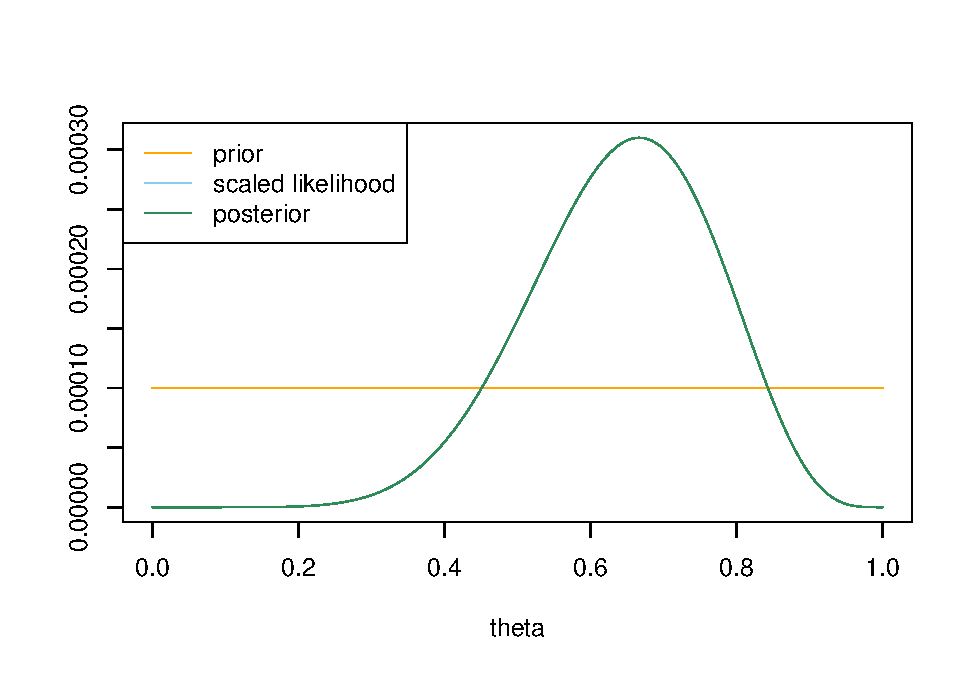
\includegraphics{bayesian-reasoning-and-methods_files/figure-latex/unnamed-chunk-41-1.pdf}
\item
  See plot below. The posterior is a compromise between the ``triangular'' prior which places highest prior probability near 0.5, and the likelihood. For this posterior, the posterior probability is greater near 0.5 than for the one in the previous part.

\begin{Shaded}
\begin{Highlighting}[]
\CommentTok{\# prior}
\NormalTok{theta =}\StringTok{ }\KeywordTok{seq}\NormalTok{(}\DecValTok{0}\NormalTok{, }\DecValTok{1}\NormalTok{, }\FloatTok{0.0001}\NormalTok{)}
\NormalTok{prior =}\StringTok{ }\DecValTok{1} \OperatorTok{{-}}\StringTok{ }\DecValTok{2} \OperatorTok{*}\StringTok{ }\KeywordTok{abs}\NormalTok{(theta }\OperatorTok{{-}}\StringTok{ }\FloatTok{0.5}\NormalTok{)}
\NormalTok{prior =}\StringTok{ }\NormalTok{prior }\OperatorTok{/}\StringTok{ }\KeywordTok{sum}\NormalTok{(prior)}

\CommentTok{\# data}
\NormalTok{n =}\StringTok{ }\DecValTok{12} \CommentTok{\# sample size}
\NormalTok{y =}\StringTok{ }\DecValTok{8} \CommentTok{\# sample count of success}

\CommentTok{\# likelihood, using binomial}
\NormalTok{likelihood =}\StringTok{ }\KeywordTok{dbinom}\NormalTok{(y, n, theta) }\CommentTok{\# function of theta}


\CommentTok{\# plots}
\KeywordTok{plot\_posterior}\NormalTok{(theta, prior, likelihood)}
\end{Highlighting}
\end{Shaded}

  \includegraphics{bayesian-reasoning-and-methods_files/figure-latex/unnamed-chunk-42-1.pdf}
\item
  Again the posterior is a compromise between prior and likelihood. The prior probabilities are greatest for values of \(\theta\) near 0; however, the likelihood corresponding to these values is small, so the posterior probabilities are close to 0. As in the previous part, some of the posterior probability is shifted towards part 0.5, as opposed to what happens with the uniform prior.

\begin{Shaded}
\begin{Highlighting}[]
\CommentTok{\# prior}
\NormalTok{theta =}\StringTok{ }\KeywordTok{seq}\NormalTok{(}\DecValTok{0}\NormalTok{, }\DecValTok{1}\NormalTok{, }\FloatTok{0.0001}\NormalTok{)}
\NormalTok{prior =}\StringTok{ }\DecValTok{1} \OperatorTok{{-}}\StringTok{ }\NormalTok{theta}
\NormalTok{prior =}\StringTok{ }\NormalTok{prior }\OperatorTok{/}\StringTok{ }\KeywordTok{sum}\NormalTok{(prior)}

\CommentTok{\# data}
\NormalTok{n =}\StringTok{ }\DecValTok{12} \CommentTok{\# sample size}
\NormalTok{y =}\StringTok{ }\DecValTok{8} \CommentTok{\# sample count of success}

\CommentTok{\# likelihood, using binomial}
\NormalTok{likelihood =}\StringTok{ }\KeywordTok{dbinom}\NormalTok{(y, n, theta) }\CommentTok{\# function of theta}

\CommentTok{\# plots}
\KeywordTok{plot\_posterior}\NormalTok{(theta, prior, likelihood)}
\end{Highlighting}
\end{Shaded}

  \includegraphics{bayesian-reasoning-and-methods_files/figure-latex/unnamed-chunk-43-1.pdf}
\item
  For the ``flat'' prior, the posterior is proportional to the likelihood. For the other priors, the posterior is a compromise between prior and likelihood. The prior does have some influence. We do see three somewhat different posterior distributions corresponding to these three prior distributions.
\end{enumerate}

\begin{itemize}
\tightlist
\item
  Even in situations where the data are discrete (e.g., binary success/failure data, count data), most statistical \emph{parameters} take values on a \emph{continuous} scale.
\item
  Thus in a Bayesian analysis, parameters are usually \emph{continuous random variables}, and have \emph{continuous probability distributions}, a.k.a., \emph{densities}.
\item
  An alternative to dealing with continuous distributions is to use \textbf{grid approximation}: Treat the parameter as discrete, on a sufficiently fine grid of values, and use discrete distributions.
\end{itemize}

\begin{example}
\protect\hypertarget{exm:kissing-discrete3}{}{\label{exm:kissing-discrete3} }
Continuing Example \ref{exm:kissing-mle}.
Now we'll perform a Bayesian analysis on the actual study data in which 80 couples out of a sample of 124 leaned right.
We'll again use a grid approximation and assume that any multiple of 0.0001 between 0 and 1 is a possible value of \(\theta\): \(0, 0.0001, 0.0002, \ldots, 0.9999, 1\).
\end{example}

\begin{enumerate}
\def\labelenumi{\arabic{enumi}.}
\tightlist
\item
  Before performing the Bayesian analysis, use software to plot the likelihood when \(y=80\) couples in a sample of \(n=124\) kissing couples lean right, and compute the maximum likelihood estimate of \(\theta\) based on this data.
\item
  Now back to Bayesian analysis. Assume a discrete uniform prior distribution for \(\theta\).
  Suppose that \(y=80\) couples in a sample of \(n=124\) kissing couples lean right.
  Use software to plot the prior distribution, the likelihood function, and then find the posterior and plot it. Describe the posterior distribution.
  What does it say about \(\theta\)?
\item
  Now assume a prior distribution which is proportional to \(1-2|\theta-0.5|\) for \(\theta = 0, 0.0001, 0.0002, \ldots, 0.9999, 1\).
  Then suppose again that \(y=80\) couples in a sample of \(n=124\) kissing couples lean right.
  Use software to plot the prior distribution, the likelihood function, and then find the posterior and plot it.
  What does the posterior distribution say about \(\theta\)?
\item
  Now assume a prior distribution which is proportional to \(1-\theta\) for \(\theta = 0, 0.0001, 0.0002, \ldots, 0.9999, 1\).
  Then suppose again that \(y=80\) couples in a sample of \(n=124\) kissing couples lean right.
  Use software to plot the prior distribution, the likelihood function, and then find the posterior and plot it.
  What does the posterior distribution say about \(\theta\)?
\item
  Compare the posterior distributions corresponding to the three different priors. How does each posterior distribution compare to the prior and the likelihood? Comment on the influence that the prior distribution has. Does the Bayesian inference for these data appear to be highly sensitive to the choice of prior? How does this compare to the \(n=12\) situation?
\end{enumerate}

\begin{solution}
\iffalse{} {Solution. } \fi{}to Example \ref{exm:kissing-discrete3}
\end{solution}

\begin{enumerate}
\def\labelenumi{\arabic{enumi}.}
\item
  See plot below. The likelihood function is \(f(y=80|\theta) = \binom{124}{80}\theta^{80}(1-\theta)^{124-80}, 0 \le\theta\le1\), the likelihood of observing a value of \(y=80\) from a Binomial(124, \(\theta\)) distribution (\texttt{dbinom(80,\ 124,\ theta)}). The maximum likelihood estimate of \(\theta\) is the sample proportion \(80/124=0.645\).
\item
  See plot below. Since the prior is flat, the posterior is proportional to the likelihood. The posterior places almost all of its probability on \(\theta\) values between about 0.55 and 0.75, with the highest probability near the observed sample proportion of 0.645.

\begin{Shaded}
\begin{Highlighting}[]
\CommentTok{\# prior}
\NormalTok{theta =}\StringTok{ }\KeywordTok{seq}\NormalTok{(}\DecValTok{0}\NormalTok{, }\DecValTok{1}\NormalTok{, }\FloatTok{0.0001}\NormalTok{)}
\NormalTok{prior =}\StringTok{ }\KeywordTok{rep}\NormalTok{(}\DecValTok{1}\NormalTok{, }\KeywordTok{length}\NormalTok{(theta))}
\NormalTok{prior =}\StringTok{ }\NormalTok{prior }\OperatorTok{/}\StringTok{ }\KeywordTok{sum}\NormalTok{(prior)}

\CommentTok{\# data}
\NormalTok{n =}\StringTok{ }\DecValTok{124} \CommentTok{\# sample size}
\NormalTok{y =}\StringTok{ }\DecValTok{80} \CommentTok{\# sample count of success}

\CommentTok{\# likelihood, using binomial}
\NormalTok{likelihood =}\StringTok{ }\KeywordTok{dbinom}\NormalTok{(y, n, theta) }\CommentTok{\# function of theta}

\CommentTok{\# plots}
\KeywordTok{plot\_posterior}\NormalTok{(theta, prior, likelihood)}
\end{Highlighting}
\end{Shaded}

  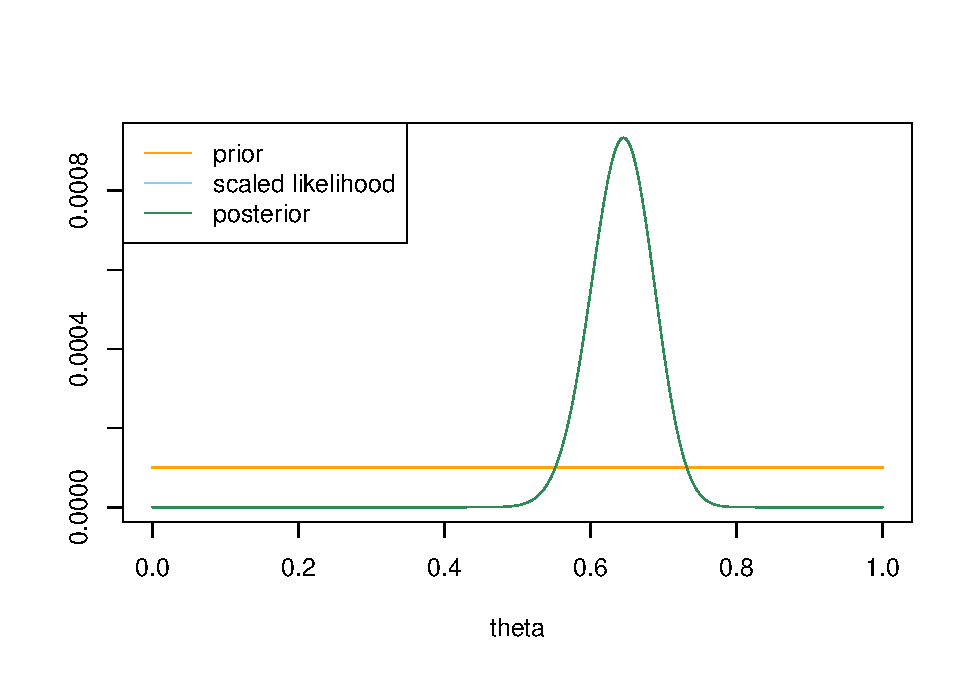
\includegraphics{bayesian-reasoning-and-methods_files/figure-latex/unnamed-chunk-44-1.pdf}
\item
  See the plot below. The posterior is very similar to the one from the previous part.

  \includegraphics{bayesian-reasoning-and-methods_files/figure-latex/unnamed-chunk-45-1.pdf}
\item
  See the plot below. The posterior is very similar to the one from the previous part.

  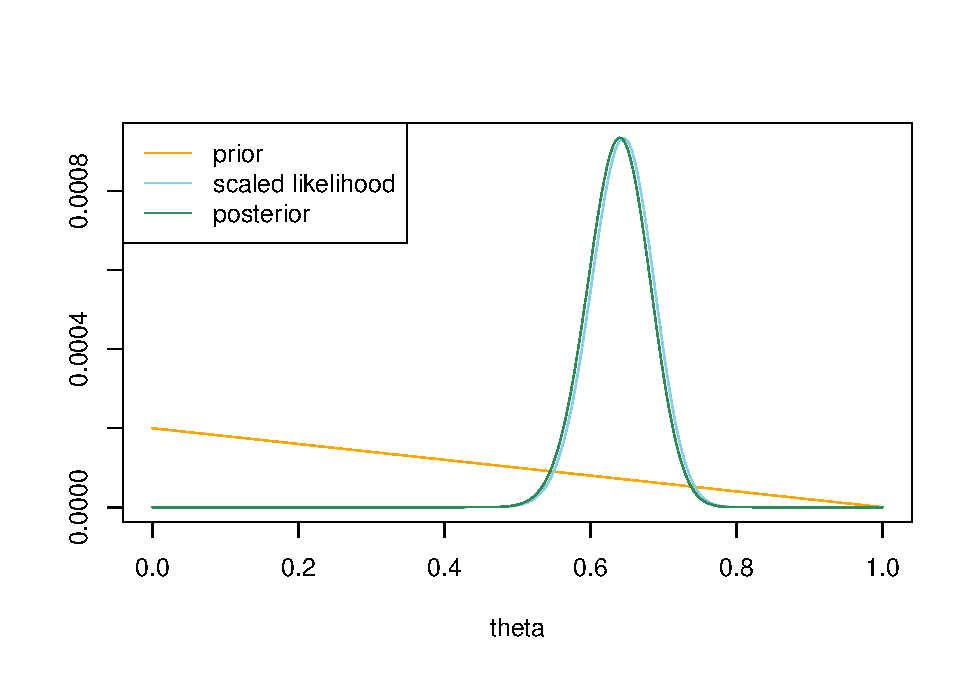
\includegraphics{bayesian-reasoning-and-methods_files/figure-latex/unnamed-chunk-46-1.pdf}
\item
  Even though the priors are different, they are all similar to each other and all similar to the shape of the likelihood. Comparing these priors it does not appear that the posterior is highly sensitive to choice of prior. The data carry more weight when \(n=124\) than it did when \(n=12\). In other words, the prior has less influence when the sample size is larger. When the sample size is larger, the likelihood is more ``peaked'' and so the likelihood, and hence posterior, is small outside a narrower range of values than when the sample size is small.
\end{enumerate}

Recall that the likelihood function is the probability (or density for continuous data) of observing the sample data \(y\) viewed as a \emph{function of the parameter} \(\theta\).
When the data \(y\) takes values on a continuous scale, the likelihood is determined by the \emph{probability density function} of \(Y\) given \(\theta\), \(f(y|\theta)\).
In the likelihood function, the observed value of the data \(y\) is treated as a fixed constant, and the likelihood of observing that \(y\) is evaluated for all potential values of \(\theta\).

Recall that a continuous random variable\footnote{Why \(U\) and not \(X\) or \(Y\)? In a Bayesian analysis, we might assume the data follows a Normal distribution, but we might also use a Normal distribution to quantify the uncertainty about a parameter. We generally associate \(X\) and \(Y\) with data. \(U\) is supposed to represent a more general variable, which could be either data or a parameter.} \(U\) follows a \textbf{Normal (a.k.a., Gaussian) distribution} with mean \(\mu\) and standard deviation \(\sigma>0\) if its probability density function is\footnote{\(\exp\) is just another way of writing the exponential function, \(\exp(u)=e^u\).}
\begin{align*}
f_U(u) & = \frac{1}{\sigma\sqrt{2\pi}}\,\exp\left(-\frac{1}{2}\left(\frac{u-\mu}{\sigma}\right)^2\right), \quad -\infty<u<\infty.\\
& \propto \frac{1}{\sigma}\,\exp\left(-\frac{1}{2}\left(\frac{u-\mu}{\sigma}\right)^2\right), \quad -\infty<u<\infty.
\end{align*}
The constant \(1/\sqrt{2\pi}\) ensures that the total area under the density is 1, but it doesn't effect the shape of the density.

In R, \texttt{dnorm(u,\ mu,\ sigma)}.

\begin{example}
\protect\hypertarget{exm:body-temp-discrete}{}{\label{exm:body-temp-discrete} }
Assume body temperatures (degrees Fahrenheit) of healthy adults follow a Normal distribution with unknown mean \(\mu\) and known\footnote{It's unrealistic to assume the population standard deviation is known. We'll consider the case of unknown standard deviation later.} standard deviation \(\sigma=1\).
Suppose we wish to estimate \(\mu\), the population mean healthy human body temperature.
\end{example}

\begin{enumerate}
\def\labelenumi{\arabic{enumi}.}
\tightlist
\item
  Assume first the following discrete prior distribution for \(\mu\) which places probability 0.10, 0.25, 0.30, 0.25, 0.10 on the values 97.6, 98.1, 98.6, 99.1, 99.6, respectively. Suppose a single temperature value of 97.9 is observed. Construct a Bayes table and find the posterior distribution of \(\mu\). In particular, how do you determine the likelihood?
\item
  Now suppose a second temperature value, 97.5, is observed, independently of the first. Construct a Bayes table and find the posterior distribution of \(\mu\) after observing these two measurements, using the posterior distribution from the previous part as the prior distribution in this part.
\item
  Now consider the original prior again.
  Determine the likelihood of observing temperatures of 97.9 and 97.5 in a sample of size 2. Then construct a Bayes table and find the posterior distribution of \(\mu\) after observing these two measurements. Compare to the previous part.
\item
  Consider the original prior again. Suppose that we take a random sample of two temperature measurements, but instead of observing the two individual values, we only observe that the sample mean is 97.7. Determine the likelihood of observing a sample mean of 97.7 in a sample of size 2. (Hint: if \(\bar{Y}\) is the sample mean of \(n\) values from a \(N(\mu, \sigma)\) distribution, what is the distribution of \(\bar{Y}\)?) Then construct a Bayes table and find the posterior distribution of \(\mu\) after observing this sample mean. Compare to the previous part.
\end{enumerate}

\begin{solution}
\iffalse{} {Solution. } \fi{}to Example \ref{exm:body-temp-discrete}
\end{solution}

\begin{enumerate}
\def\labelenumi{\arabic{enumi}.}
\item
  The likelihood is determined by evaluating the Normal(\(\mu\), 1) density at \(y=97.9\) for different values of \(\mu\): \texttt{dnorm(97.9,\ mu,\ 1)} or
  \[
  f(97.9|\mu)  = \frac{1}{\sqrt{2\pi}}\,\exp\left(-\frac{1}{2}\left(\frac{97.9-\mu}{1}\right)^2\right)
  \]
  See the table below. Posterior probability is shifted towards the smaller values of \(\mu\) since those give the higher likelihood of the observed value \(y=97.9\).

\begin{Shaded}
\begin{Highlighting}[]
\CommentTok{\# prior}
\NormalTok{theta =}\StringTok{ }\KeywordTok{seq}\NormalTok{(}\FloatTok{97.6}\NormalTok{, }\FloatTok{99.6}\NormalTok{, }\FloatTok{0.5}\NormalTok{)}
\NormalTok{prior =}\StringTok{ }\KeywordTok{c}\NormalTok{(}\FloatTok{0.10}\NormalTok{, }\FloatTok{0.25}\NormalTok{, }\FloatTok{0.30}\NormalTok{, }\FloatTok{0.25}\NormalTok{, }\FloatTok{0.10}\NormalTok{)}
\NormalTok{prior =}\StringTok{ }\NormalTok{prior }\OperatorTok{/}\StringTok{ }\KeywordTok{sum}\NormalTok{(prior)}

\CommentTok{\# data}
\NormalTok{y =}\StringTok{ }\FloatTok{97.9} \CommentTok{\# single observed value}
\NormalTok{sigma =}\StringTok{ }\DecValTok{1}


\CommentTok{\# likelihood}
\NormalTok{likelihood =}\StringTok{ }\KeywordTok{dnorm}\NormalTok{(y, theta, sigma) }\CommentTok{\# function of theta}

\CommentTok{\# posterior}
\NormalTok{product =}\StringTok{ }\NormalTok{likelihood }\OperatorTok{*}\StringTok{ }\NormalTok{prior}
\NormalTok{posterior =}\StringTok{ }\NormalTok{product }\OperatorTok{/}\StringTok{ }\KeywordTok{sum}\NormalTok{(product)}

\CommentTok{\# bayes table}
\NormalTok{bayes\_table =}\StringTok{ }\KeywordTok{data.frame}\NormalTok{(theta,}
\NormalTok{                     prior,}
\NormalTok{                     likelihood,}
\NormalTok{                     product,}
\NormalTok{                     posterior)}

\KeywordTok{kable}\NormalTok{(bayes\_table, }\DataTypeTok{digits =} \DecValTok{4}\NormalTok{, }\DataTypeTok{align =} \StringTok{\textquotesingle{}r\textquotesingle{}}\NormalTok{)}
\end{Highlighting}
\end{Shaded}

  \begin{tabular}{r|r|r|r|r}
   \hline
   theta & prior & likelihood & product & posterior\\
   \hline
   97.6 & 0.10 & 0.3814 & 0.0381 & 0.1326\\
   \hline
   98.1 & 0.25 & 0.3910 & 0.0978 & 0.3400\\
   \hline
   98.6 & 0.30 & 0.3123 & 0.0937 & 0.3258\\
   \hline
   99.1 & 0.25 & 0.1942 & 0.0485 & 0.1688\\
   \hline
   99.6 & 0.10 & 0.0940 & 0.0094 & 0.0327\\
   \hline
   \end{tabular}
\item
  See the table below. More posterior probability is shifted towards the smaller values of \(\mu\).

\begin{Shaded}
\begin{Highlighting}[]
\CommentTok{\# prior}
\NormalTok{prior =}\StringTok{ }\NormalTok{posterior}

\CommentTok{\# data}
\NormalTok{y =}\StringTok{ }\FloatTok{97.5} \CommentTok{\# single observed value}
\NormalTok{sigma =}\StringTok{ }\DecValTok{1}


\CommentTok{\# likelihood}
\NormalTok{likelihood =}\StringTok{ }\KeywordTok{dnorm}\NormalTok{(y, theta, sigma) }\CommentTok{\# function of theta}

\CommentTok{\# posterior}
\NormalTok{product =}\StringTok{ }\NormalTok{likelihood }\OperatorTok{*}\StringTok{ }\NormalTok{prior}
\NormalTok{posterior =}\StringTok{ }\NormalTok{product }\OperatorTok{/}\StringTok{ }\KeywordTok{sum}\NormalTok{(product)}

\CommentTok{\# bayes table}
\NormalTok{bayes\_table =}\StringTok{ }\KeywordTok{data.frame}\NormalTok{(theta,}
\NormalTok{                     prior,}
\NormalTok{                     likelihood,}
\NormalTok{                     product,}
\NormalTok{                     posterior)}

\KeywordTok{kable}\NormalTok{(bayes\_table, }\DataTypeTok{digits =} \DecValTok{4}\NormalTok{, }\DataTypeTok{align =} \StringTok{\textquotesingle{}r\textquotesingle{}}\NormalTok{)}
\end{Highlighting}
\end{Shaded}

  \begin{tabular}{r|r|r|r|r}
   \hline
   theta & prior & likelihood & product & posterior\\
   \hline
   97.6 & 0.1326 & 0.3970 & 0.0527 & 0.2048\\
   \hline
   98.1 & 0.3400 & 0.3332 & 0.1133 & 0.4407\\
   \hline
   98.6 & 0.3258 & 0.2179 & 0.0710 & 0.2761\\
   \hline
   99.1 & 0.1688 & 0.1109 & 0.0187 & 0.0728\\
   \hline
   99.6 & 0.0327 & 0.0440 & 0.0014 & 0.0056\\
   \hline
   \end{tabular}
\item
  See the table below.
  Since the two measurements are independent, the likelihood is the product of the likelihoods for \(y=97.9\) and \(y=97.5\).
  The posterior is the same in the previous part. It doesn't matter if we update the posterior after each observations, or all at once.

\begin{Shaded}
\begin{Highlighting}[]
\CommentTok{\# prior}
\NormalTok{theta =}\StringTok{ }\KeywordTok{seq}\NormalTok{(}\FloatTok{97.6}\NormalTok{, }\FloatTok{99.6}\NormalTok{, }\FloatTok{0.5}\NormalTok{)}
\NormalTok{prior =}\StringTok{ }\KeywordTok{c}\NormalTok{(}\FloatTok{0.10}\NormalTok{, }\FloatTok{0.25}\NormalTok{, }\FloatTok{0.30}\NormalTok{, }\FloatTok{0.25}\NormalTok{, }\FloatTok{0.10}\NormalTok{)}
\NormalTok{prior =}\StringTok{ }\NormalTok{prior }\OperatorTok{/}\StringTok{ }\KeywordTok{sum}\NormalTok{(prior)}

\CommentTok{\# data}
\NormalTok{y =}\StringTok{ }\KeywordTok{c}\NormalTok{(}\FloatTok{97.9}\NormalTok{, }\FloatTok{97.5}\NormalTok{) }\CommentTok{\# two observed values}
\NormalTok{sigma =}\StringTok{ }\DecValTok{1}


\CommentTok{\# likelihood}
\NormalTok{likelihood =}\StringTok{ }\KeywordTok{dnorm}\NormalTok{(y[}\DecValTok{1}\NormalTok{], theta, sigma) }\OperatorTok{*}\StringTok{ }\KeywordTok{dnorm}\NormalTok{(y[}\DecValTok{2}\NormalTok{], theta, sigma)  }\CommentTok{\# function of theta}

\CommentTok{\# posterior}
\NormalTok{product =}\StringTok{ }\NormalTok{likelihood }\OperatorTok{*}\StringTok{ }\NormalTok{prior}
\NormalTok{posterior =}\StringTok{ }\NormalTok{product }\OperatorTok{/}\StringTok{ }\KeywordTok{sum}\NormalTok{(product)}

\CommentTok{\# bayes table}
\NormalTok{bayes\_table =}\StringTok{ }\KeywordTok{data.frame}\NormalTok{(theta,}
\NormalTok{                     prior,}
\NormalTok{                     likelihood,}
\NormalTok{                     product,}
\NormalTok{                     posterior)}

\KeywordTok{kable}\NormalTok{(bayes\_table, }\DataTypeTok{digits =} \DecValTok{4}\NormalTok{, }\DataTypeTok{align =} \StringTok{\textquotesingle{}r\textquotesingle{}}\NormalTok{)}
\end{Highlighting}
\end{Shaded}

  \begin{tabular}{r|r|r|r|r}
   \hline
   theta & prior & likelihood & product & posterior\\
   \hline
   97.6 & 0.10 & 0.1514 & 0.0151 & 0.2048\\
   \hline
   98.1 & 0.25 & 0.1303 & 0.0326 & 0.4407\\
   \hline
   98.6 & 0.30 & 0.0680 & 0.0204 & 0.2761\\
   \hline
   99.1 & 0.25 & 0.0215 & 0.0054 & 0.0728\\
   \hline
   99.6 & 0.10 & 0.0041 & 0.0004 & 0.0056\\
   \hline
   \end{tabular}
\item
  For a sample of size \(n\) from a \(N(\mu,\sigma)\) distribution, the sample mean follows a \(N\left(\mu, \frac{\sigma}{\sqrt{n}}\right)\) distribution. The likelihood is determined by evaluating the Normal(\(\mu\), \(\frac{1}{\sqrt{2}}\)) density at \(y=97.7\) for different values of \(\mu\): \texttt{dnorm(97.7,\ mu,\ 1\ /\ sqrt(2))} or
  \[
  f_{\bar{Y}}(97.7|\mu)  \propto \exp\left(-\frac{1}{2}\left(\frac{97.7-\mu}{1/\sqrt{2}}\right)^2\right)
  \]
  See the table below. While the likelihood is not the same as in the previous part, it is \emph{proportionally} the same; that is, the likelihood in this part has the same \emph{shape} as the likelihood in the previous part. Therefore, the posterior distributions are the same.

\begin{Shaded}
\begin{Highlighting}[]
\CommentTok{\# prior}
\NormalTok{theta =}\StringTok{ }\KeywordTok{seq}\NormalTok{(}\FloatTok{97.6}\NormalTok{, }\FloatTok{99.6}\NormalTok{, }\FloatTok{0.5}\NormalTok{)}
\NormalTok{prior =}\StringTok{ }\KeywordTok{c}\NormalTok{(}\FloatTok{0.10}\NormalTok{, }\FloatTok{0.25}\NormalTok{, }\FloatTok{0.30}\NormalTok{, }\FloatTok{0.25}\NormalTok{, }\FloatTok{0.10}\NormalTok{)}
\NormalTok{prior =}\StringTok{ }\NormalTok{prior }\OperatorTok{/}\StringTok{ }\KeywordTok{sum}\NormalTok{(prior)}

\CommentTok{\# data}
\NormalTok{n =}\StringTok{ }\DecValTok{2}
\NormalTok{y =}\StringTok{ }\FloatTok{97.7} \CommentTok{\# sample mean}
\NormalTok{sigma =}\StringTok{ }\DecValTok{1}


\CommentTok{\# likelihood}
\NormalTok{likelihood =}\StringTok{ }\KeywordTok{dnorm}\NormalTok{(y, theta, sigma }\OperatorTok{/}\StringTok{ }\KeywordTok{sqrt}\NormalTok{(n)) }\CommentTok{\# function of theta}

\CommentTok{\# posterior}
\NormalTok{product =}\StringTok{ }\NormalTok{likelihood }\OperatorTok{*}\StringTok{ }\NormalTok{prior}
\NormalTok{posterior =}\StringTok{ }\NormalTok{product }\OperatorTok{/}\StringTok{ }\KeywordTok{sum}\NormalTok{(product)}

\CommentTok{\# bayes table}
\NormalTok{bayes\_table =}\StringTok{ }\KeywordTok{data.frame}\NormalTok{(theta,}
\NormalTok{                     prior,}
\NormalTok{                     likelihood,}
\NormalTok{                     product,}
\NormalTok{                     posterior)}

\KeywordTok{kable}\NormalTok{(bayes\_table, }\DataTypeTok{digits =} \DecValTok{4}\NormalTok{, }\DataTypeTok{align =} \StringTok{\textquotesingle{}r\textquotesingle{}}\NormalTok{)}
\end{Highlighting}
\end{Shaded}

  \begin{tabular}{r|r|r|r|r}
   \hline
   theta & prior & likelihood & product & posterior\\
   \hline
   97.6 & 0.10 & 0.5586 & 0.0559 & 0.2048\\
   \hline
   98.1 & 0.25 & 0.4808 & 0.1202 & 0.4407\\
   \hline
   98.6 & 0.30 & 0.2510 & 0.0753 & 0.2761\\
   \hline
   99.1 & 0.25 & 0.0795 & 0.0199 & 0.0728\\
   \hline
   99.6 & 0.10 & 0.0153 & 0.0015 & 0.0056\\
   \hline
   \end{tabular}
\end{enumerate}

It is often not necessary to know all the individual data values to evaluate the \emph{shape} of the likelihood as a function of the parameter \(\theta\), but rather simply the values of a few summary statistics.\\
For example, when estimating the population mean of a Normal distribution with known standard deviation \(\sigma\), it is sufficient to know the sample mean for the purposes of evaluating the shape of the likelihood of the observed data under different potential values of the population mean.

If \(Y_1, \ldots, Y_n\) is a random sample from a \(N(\mu, \sigma)\) distribution, then \(\bar{Y}\) has a \(N\left(\mu, \frac{\sigma}{\sqrt{n}}\right)\) distribution

\begin{itemize}
\tightlist
\item
  \(\sigma\) measures the unit-to-unit variability of individual values of the variable over all possible units in the population. For example, how much do body temperatures vary from person-to-person over many people?
\item
  \(\frac{\sigma}{\sqrt{n}}\) measures the sample-to-sample variability of sample means over all possible samples of size \(n\) from the population. For example, how much do sample mean body temperatures from sample to sample over many samples of \(n\) people?
\end{itemize}

\begin{example}
\protect\hypertarget{exm:body-temp-discrete2}{}{\label{exm:body-temp-discrete2} }
Continuing the previous example. We'll now use a grid approximation and assume that any multiple of 0.0001 between 96.0 and 100.0 is a possible value of \(\mu\): \(96.0, 96.0001, 96.0002, \ldots, 99.9999, 100.0\).
\end{example}

\begin{enumerate}
\def\labelenumi{\arabic{enumi}.}
\tightlist
\item
  Assume a discrete uniform prior distribution over \(\mu\) values in the grid.
  Suppose that the sample mean temperature is \(\bar{y}=97.7\) in a sample of \(n=2\) temperature measurements.
  Use software to plot the prior distribution, the (scaled) likelihood function, and then find the posterior and plot it. Describe the posterior distribution.
  What does it say about \(\mu\)?
\item
  Now assume a prior distribution which is proportional to a Normal distribution with mean 98.6 and standard deviation 0.7 over \(\mu\) values in the grid.
  Suppose that the sample mean temperature is \(\bar{y}=97.7\) in a sample of \(n=2\) temperature measurements.
  Use software to plot the prior distribution, the (scaled) likelihood function, and then find the posterior and plot it. Describe the posterior distribution.
  What does it say about \(\mu\)?
\item
  Compare the posterior distributions corresponding to the two different priors. How does each posterior distribution compare to the prior and the likelihood? Comment on the influence that the prior distribution has.
\end{enumerate}

\begin{solution}
\iffalse{} {Solution. } \fi{}to Example \ref{exm:body-temp-discrete2}
\end{solution}

\begin{enumerate}
\def\labelenumi{\arabic{enumi}.}
\item
  Since the prior is flat, the posterior has the same shape as the likelihood. The highest posterior probability is near the observed sample mean of 97.7.

\begin{Shaded}
\begin{Highlighting}[]
\CommentTok{\# prior}
\NormalTok{theta =}\StringTok{ }\KeywordTok{seq}\NormalTok{(}\DecValTok{96}\NormalTok{, }\DecValTok{100}\NormalTok{, }\FloatTok{0.0001}\NormalTok{)}
\NormalTok{prior =}\StringTok{ }\KeywordTok{rep}\NormalTok{(}\DecValTok{1}\NormalTok{, }\KeywordTok{length}\NormalTok{(theta))}
\NormalTok{prior =}\StringTok{ }\NormalTok{prior }\OperatorTok{/}\StringTok{ }\KeywordTok{sum}\NormalTok{(prior)}

\CommentTok{\# data}
\NormalTok{n =}\StringTok{ }\DecValTok{2} \CommentTok{\# sample size}
\NormalTok{y =}\StringTok{ }\FloatTok{97.7} \CommentTok{\# sample mean}
\NormalTok{sigma =}\StringTok{ }\DecValTok{1}

\CommentTok{\# likelihood}
\NormalTok{likelihood =}\StringTok{ }\KeywordTok{dnorm}\NormalTok{(y, theta, sigma }\OperatorTok{/}\StringTok{ }\KeywordTok{sqrt}\NormalTok{(n)) }\CommentTok{\# function of theta}

\CommentTok{\# plots}
\NormalTok{plot\_posterior \textless{}{-}}\StringTok{ }\ControlFlowTok{function}\NormalTok{(theta, prior, likelihood)\{}

  \CommentTok{\# posterior}
\NormalTok{  product =}\StringTok{ }\NormalTok{likelihood }\OperatorTok{*}\StringTok{ }\NormalTok{prior}
\NormalTok{  posterior =}\StringTok{ }\NormalTok{product }\OperatorTok{/}\StringTok{ }\KeywordTok{sum}\NormalTok{(product)}

\NormalTok{  ylim =}\StringTok{ }\KeywordTok{c}\NormalTok{(}\DecValTok{0}\NormalTok{, }\KeywordTok{max}\NormalTok{(}\KeywordTok{c}\NormalTok{(prior, posterior, likelihood }\OperatorTok{/}\StringTok{ }\KeywordTok{sum}\NormalTok{(likelihood))))}
  \KeywordTok{plot}\NormalTok{(theta, prior, }\DataTypeTok{type=}\StringTok{\textquotesingle{}l\textquotesingle{}}\NormalTok{, }\DataTypeTok{xlim=}\KeywordTok{range}\NormalTok{(theta), }\DataTypeTok{ylim=}\NormalTok{ylim, }\DataTypeTok{col=}\StringTok{"orange"}\NormalTok{, }\DataTypeTok{xlab=}\StringTok{\textquotesingle{}theta\textquotesingle{}}\NormalTok{, }\DataTypeTok{ylab=}\StringTok{\textquotesingle{}\textquotesingle{}}\NormalTok{)}
  \KeywordTok{par}\NormalTok{(}\DataTypeTok{new=}\NormalTok{T) }
  \KeywordTok{plot}\NormalTok{(theta, likelihood}\OperatorTok{/}\KeywordTok{sum}\NormalTok{(likelihood), }\DataTypeTok{type=}\StringTok{\textquotesingle{}l\textquotesingle{}}\NormalTok{, }\DataTypeTok{xlim=}\KeywordTok{range}\NormalTok{(theta), }\DataTypeTok{ylim=}\NormalTok{ylim, }\DataTypeTok{col=}\StringTok{"skyblue"}\NormalTok{, }\DataTypeTok{xlab=}\StringTok{\textquotesingle{}\textquotesingle{}}\NormalTok{, }\DataTypeTok{ylab=}\StringTok{\textquotesingle{}\textquotesingle{}}\NormalTok{)}
  \KeywordTok{par}\NormalTok{(}\DataTypeTok{new=}\NormalTok{T)}
  \KeywordTok{plot}\NormalTok{(theta, posterior, }\DataTypeTok{type=}\StringTok{\textquotesingle{}l\textquotesingle{}}\NormalTok{, }\DataTypeTok{xlim=}\KeywordTok{range}\NormalTok{(theta), }\DataTypeTok{ylim=}\NormalTok{ylim, }\DataTypeTok{col=}\StringTok{"seagreen"}\NormalTok{, }\DataTypeTok{xlab=}\StringTok{\textquotesingle{}\textquotesingle{}}\NormalTok{, }\DataTypeTok{ylab=}\StringTok{\textquotesingle{}\textquotesingle{}}\NormalTok{)}
  \KeywordTok{legend}\NormalTok{(}\StringTok{"topleft"}\NormalTok{, }\KeywordTok{c}\NormalTok{(}\StringTok{"prior"}\NormalTok{, }\StringTok{"scaled likelihood"}\NormalTok{, }\StringTok{"posterior"}\NormalTok{), }\DataTypeTok{lty=}\DecValTok{1}\NormalTok{, }\DataTypeTok{col=}\KeywordTok{c}\NormalTok{(}\StringTok{"orange"}\NormalTok{, }\StringTok{"skyblue"}\NormalTok{, }\StringTok{"seagreen"}\NormalTok{))}
\NormalTok{\}}

\KeywordTok{plot\_posterior}\NormalTok{(theta, prior, likelihood)}
\end{Highlighting}
\end{Shaded}

  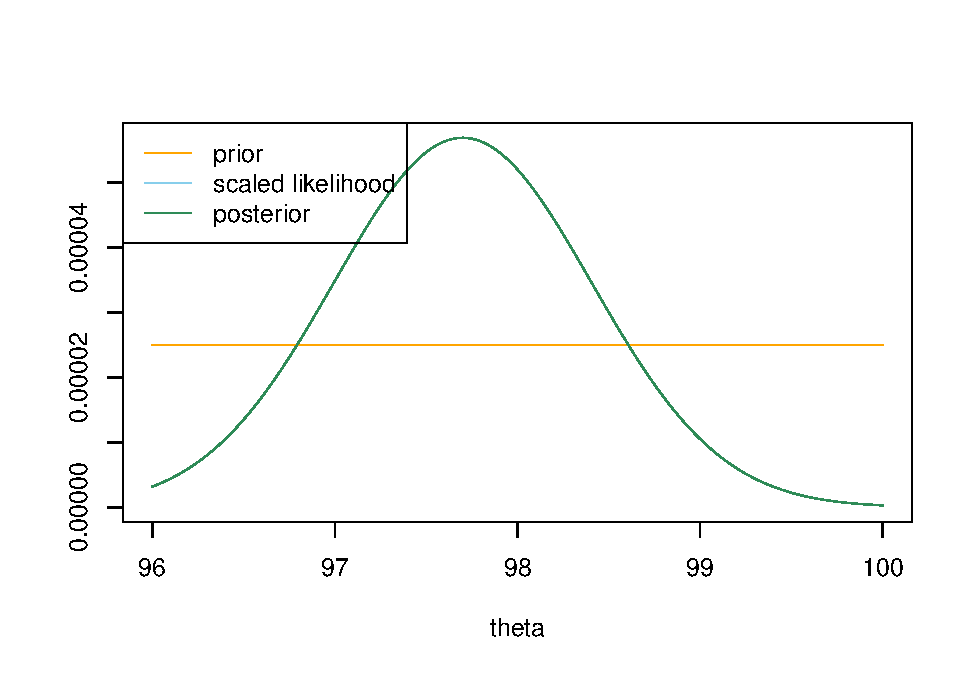
\includegraphics{bayesian-reasoning-and-methods_files/figure-latex/unnamed-chunk-51-1.pdf}
\item
  Be sure to distinguish between the Normal distribution in the prior, which quantifies our prior uncertainty about \(\mu\), and the Normal distribution used to determine the likelihood which models variability of temperatures in the population. The poster is a compromise between likelihood and prior.

\begin{Shaded}
\begin{Highlighting}[]
\CommentTok{\# prior}
\NormalTok{theta =}\StringTok{ }\KeywordTok{seq}\NormalTok{(}\DecValTok{96}\NormalTok{, }\DecValTok{100}\NormalTok{, }\FloatTok{0.0001}\NormalTok{)}
\NormalTok{prior =}\StringTok{ }\KeywordTok{dnorm}\NormalTok{(theta, }\FloatTok{98.6}\NormalTok{, }\FloatTok{0.7}\NormalTok{)}
\NormalTok{prior =}\StringTok{ }\NormalTok{prior }\OperatorTok{/}\StringTok{ }\KeywordTok{sum}\NormalTok{(prior)}

\CommentTok{\# data}
\NormalTok{n =}\StringTok{ }\DecValTok{2} \CommentTok{\# sample size}
\NormalTok{y =}\StringTok{ }\FloatTok{97.7} \CommentTok{\# sample mean}
\NormalTok{sigma =}\StringTok{ }\DecValTok{1}

\CommentTok{\# likelihood}
\NormalTok{likelihood =}\StringTok{ }\KeywordTok{dnorm}\NormalTok{(y, theta, sigma }\OperatorTok{/}\StringTok{ }\KeywordTok{sqrt}\NormalTok{(n)) }\CommentTok{\# function of theta}

\KeywordTok{plot\_posterior}\NormalTok{(theta, prior, likelihood)}
\end{Highlighting}
\end{Shaded}

  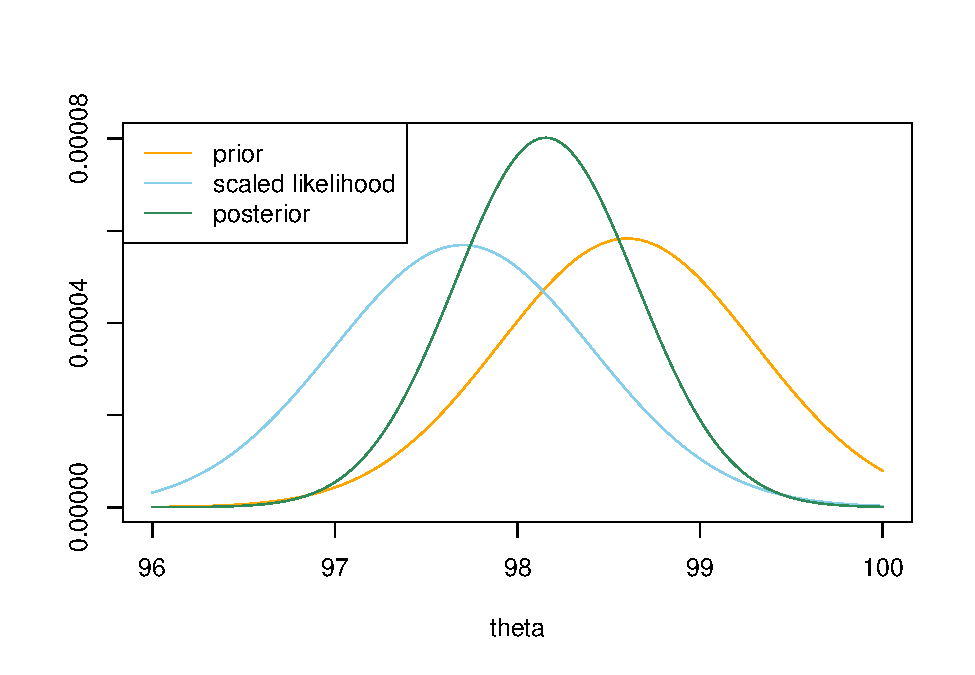
\includegraphics{bayesian-reasoning-and-methods_files/figure-latex/unnamed-chunk-52-1.pdf}
\item
  When the prior is flat, the posterior has the shape of the likelihood. Otherwise, the posterior is a compromise between prior and likelihood. When the sample size is so small, the prior will have a lot of influence on the posterior.
\end{enumerate}

\begin{example}
\protect\hypertarget{exm:body-temp-discrete3}{}{\label{exm:body-temp-discrete3} }
Continuing the previous example.
In a recent study\footnote{\href{https://www.ncbi.nlm.nih.gov/pmc/articles/PMC6258625/}{Source} and a \href{https://www.scientificamerican.com/article/are-human-body-temperatures-cooling-down/}{related article}.}, the sample mean body temperature in a sample of 208 healthy adults was 97.7 degrees F.

We'll again use a grid approximation and assume that any multiple of 0.0001 between 96.0 and 100.0 is a possible value of \(\mu\): \(96.0, 96.0001, 96.0002, \ldots, 99.9999, 100.0\).
\end{example}

\begin{enumerate}
\def\labelenumi{\arabic{enumi}.}
\tightlist
\item
  Before performing a Bayesian analysis, use software to plot the likelihood, and compute the maximum likelihood estimate of \(\mu\) based on this data.
\item
  Assume a discrete uniform prior distribution over \(\mu\) values in the grid.
  Use software to plot the prior distribution, the (scaled) likelihood function, and then find the posterior and plot it. Describe the posterior distribution.
  What does it say about \(\mu\)?
\item
  Now assume a prior distribution which is proportional a Normal distribution with mean 98.6 and standard deviation 0.7 over \(\mu\) values in the grid.
  Use software to plot the prior distribution, the (scaled) likelihood function, and then find the posterior and plot it. Describe the posterior distribution.
  What does it say about \(\mu\)?
\item
  Compare the posterior distributions corresponding to the two different priors. How does each posterior distribution compare to the prior and the likelihood? Comment on the influence that the prior distribution has. How does this compare to the \(n=2\) situation?
\end{enumerate}

\begin{solution}
\iffalse{} {Solution. } \fi{}to Example \ref{exm:body-temp-discrete3}
\end{solution}

\begin{enumerate}
\def\labelenumi{\arabic{enumi}.}
\item
  The likelihood is determined by evaluating the Normal(\(\mu\), \(\frac{1}{\sqrt{208}}\)) density at \(y=97.7\) for different values of \(\mu\): \texttt{dnorm(97.7,\ mu,\ 1\ /\ sqrt(208))} or
  \[
  f_{\bar{Y}}(97.7|\mu)  \propto \exp\left(-\frac{1}{2}\left(\frac{97.7-\mu}{1/\sqrt{208}}\right)^2\right)
  \] See a plot of the likelihood below. The MLE of \(\mu\) is the observed sample mean of 97.7.
\item
  Since the prior is flat, the posterior has the same shape as the likelihood.
  With such a large sample size, the likelihood is pretty peaked.
  So the posterior probability is concentrated in a fairly narrow range of values around 97.7.

\begin{Shaded}
\begin{Highlighting}[]
\CommentTok{\# prior}
\NormalTok{theta =}\StringTok{ }\KeywordTok{seq}\NormalTok{(}\DecValTok{96}\NormalTok{, }\DecValTok{100}\NormalTok{, }\FloatTok{0.0001}\NormalTok{)}
\NormalTok{prior =}\StringTok{ }\KeywordTok{rep}\NormalTok{(}\DecValTok{1}\NormalTok{, }\KeywordTok{length}\NormalTok{(theta))}
\NormalTok{prior =}\StringTok{ }\NormalTok{prior }\OperatorTok{/}\StringTok{ }\KeywordTok{sum}\NormalTok{(prior)}

\CommentTok{\# data}
\NormalTok{n =}\StringTok{ }\DecValTok{208} \CommentTok{\# sample size}
\NormalTok{y =}\StringTok{ }\FloatTok{97.7} \CommentTok{\# sample mean}
\NormalTok{sigma =}\StringTok{ }\DecValTok{1}

\CommentTok{\# likelihood}
\NormalTok{likelihood =}\StringTok{ }\KeywordTok{dnorm}\NormalTok{(y, theta, sigma }\OperatorTok{/}\StringTok{ }\KeywordTok{sqrt}\NormalTok{(n)) }\CommentTok{\# function of theta}

\KeywordTok{plot\_posterior}\NormalTok{(theta, prior, likelihood)}
\end{Highlighting}
\end{Shaded}

  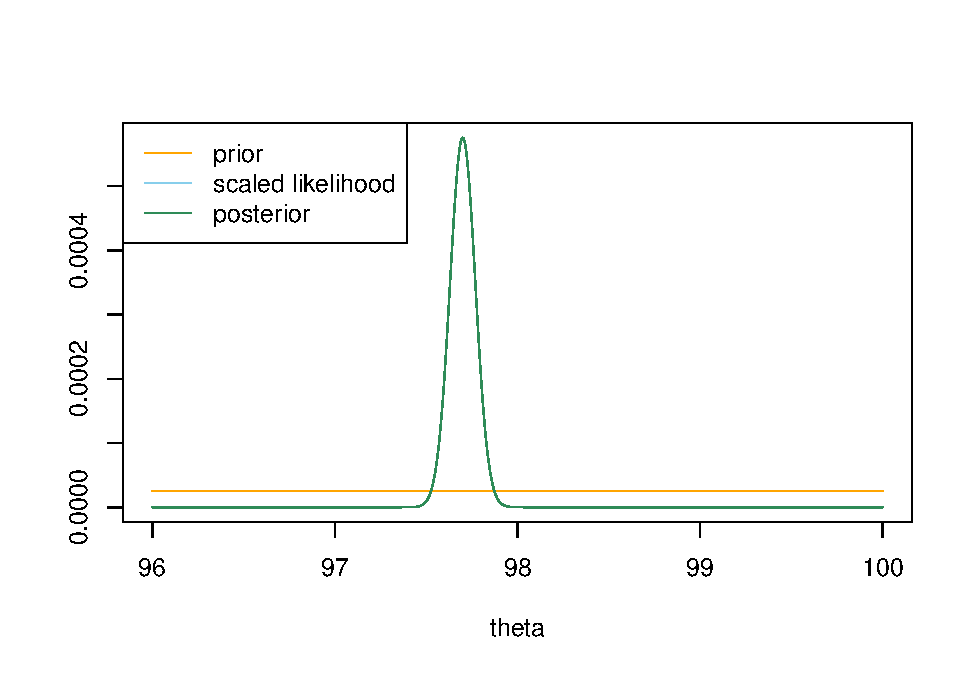
\includegraphics{bayesian-reasoning-and-methods_files/figure-latex/unnamed-chunk-53-1.pdf}
\item
  Even though the prior probability is highest near 98.6, the likelihood at these values is so small that they have small posterior probability. The posterior distribution is about the same as in the previous part.

\begin{Shaded}
\begin{Highlighting}[]
\CommentTok{\# prior}
\NormalTok{theta =}\StringTok{ }\KeywordTok{seq}\NormalTok{(}\DecValTok{96}\NormalTok{, }\DecValTok{100}\NormalTok{, }\FloatTok{0.0001}\NormalTok{)}
\NormalTok{prior =}\StringTok{ }\KeywordTok{dnorm}\NormalTok{(theta, }\FloatTok{98.6}\NormalTok{, }\FloatTok{0.7}\NormalTok{)}
\NormalTok{prior =}\StringTok{ }\NormalTok{prior }\OperatorTok{/}\StringTok{ }\KeywordTok{sum}\NormalTok{(prior)}

\CommentTok{\# data}
\NormalTok{n =}\StringTok{ }\DecValTok{208} \CommentTok{\# sample size}
\NormalTok{y =}\StringTok{ }\FloatTok{97.7} \CommentTok{\# sample mean}
\NormalTok{sigma =}\StringTok{ }\DecValTok{1}

\CommentTok{\# likelihood}
\NormalTok{likelihood =}\StringTok{ }\KeywordTok{dnorm}\NormalTok{(y, theta, sigma }\OperatorTok{/}\StringTok{ }\KeywordTok{sqrt}\NormalTok{(n)) }\CommentTok{\# function of theta}

\KeywordTok{plot\_posterior}\NormalTok{(theta, prior, likelihood)}
\end{Highlighting}
\end{Shaded}

  \includegraphics{bayesian-reasoning-and-methods_files/figure-latex/unnamed-chunk-54-1.pdf}
\item
  The posterior distributions are about the same in each case. With a large sample size, the likelihood is fairly peaked, and so the likelihood is close to 0 outside of a narrow range of values around the observed sample mean of 97.7. Therefore, the posterior probability is concentrated in this range, regardless of the prior.
\end{enumerate}

\hypertarget{inference}{%
\chapter{Introduction to Inference}\label{inference}}

In a Bayesian analysis, the posterior distribution contains all relevant information about parameters after observing sample data. We often use certain summary characteristics of the posterior distribution to make inferences about parameters.

\begin{example}
\protect\hypertarget{exm:kissing-summary}{}{\label{exm:kissing-summary} }
Continuing the kissing study in Example \ref{exm:kissing-discrete1} where \(\theta\) can only take values 0.1, 0.3, 0.5, 0.7, 0.9.
Consider a prior distribution which places probability 1/9, 2/9, 3/9, 2/9, 1/9 on the values 0.1, 0.3, 0.5, 0.7, 0.9, respectively.
\end{example}

\begin{enumerate}
\def\labelenumi{\arabic{enumi}.}
\item
  Find the mode of the prior distribution of \(\theta\), a.k.a., the ``prior mode''.
\item
  Find the median of the prior distribution of \(\theta\), a.k.a., the ``prior median''.
\item
  Find the expected value of the prior distribution of \(\theta\), a.k.a., the ``prior mean''.
\item
  Find the variance of the prior distribution \(\theta\), a.k.a, the ``prior variance''.
\item
  Find the standard deviation of the prior distribution of \(\theta\), a.k.a, the ``prior standard deviation''.

  Now suppose that \(y=8\) couples in a sample of size \(n=12\) lean right. Recall the Bayes table.

  \begin{tabular}{r|r|r|r|r}
   \hline
   theta & prior & likelihood & product & posterior\\
   \hline
   0.1 & 0.1111 & 0.0000 & 0.0000 & 0.0000\\
   \hline
   0.3 & 0.2222 & 0.0078 & 0.0017 & 0.0181\\
   \hline
   0.5 & 0.3333 & 0.1208 & 0.0403 & 0.4207\\
   \hline
   0.7 & 0.2222 & 0.2311 & 0.0514 & 0.5365\\
   \hline
   0.9 & 0.1111 & 0.0213 & 0.0024 & 0.0247\\
   \hline
   \end{tabular}
\item
  Find the mode of the posterior distribution of \(\theta\), a.k.a., the ``posterior mode''.
\item
  Find the median of the posterior distribution of \(\theta\), a.k.a., the ``posterior median''.
\item
  Find the expected value of the posterior distribution of \(\theta\), a.k.a., the ``posterior mean''.
\item
  Find the variance of the posterior distribution \(\theta\), a.k.a, the ``posterior variance''.
\item
  Find the standard deviation of the posterior distribution of \(\theta\), a.k.a, the ``posterior standard deviation''.
\item
  How have the posterior values changed from the respective prior values?
\end{enumerate}

\begin{solution}
\iffalse{} {Solution. } \fi{}to Example \ref{exm:kissing-summary}
\end{solution}

Show/hide solution

\begin{enumerate}
\def\labelenumi{\arabic{enumi}.}
\item
  The prior mode is 0.5, the value of \(\theta\) with the greatest prior probability.
\item
  The prior median is 0.5. (Add up the prior probabilities until they go from below 0.5 to above 0.5. This happens when you add in the prior probability for \(\theta=0.5\).)
\item
  The prior mean is 0.5. Remember that an expected value is a probability-weighted average value
  \[
  0.1(1/9) + 0.3(2/9) + 0.5(3/9) + 0.7(2/9) + 0.9(1/9) = 0.5.
  \]
\item
  The prior variance is 0.0533. Remember that variance is the probability-weighted average squared deviation from the mean
  \[
  (0.1-0.5)^2(1/9) + (0.3 - 0.5)^2(2/9) + (0.5-0.5)^2(3/9) + (0.7-0.5)^2(2/9) + (0.9-0.5)^2(1/9) = 0.0533
  \]
\item
  The prior standard deviation is 0.231. Remember that standard deviation is the square root of the variance: \(\sqrt{0.0533} = 0.231\).
\item
  The posterior mode is 0.7, the value of \(\theta\) with the greatest posterior probability.
\item
  The posterior median is 0.7. (Add up the posterior probabilities until they go from below 0.5 to above 0.5. This happens when you add in the posterior probability for \(\theta=0.5\).)
\item
  The posterior mean is 0.614. Now the posterior probabilities are used in the probability-weighted average value
  \[
  0.1(0.000) + 0.3(0.018) + 0.5(0.421) + 0.7(0.536) + 0.9(0.025) = 0.614.
  \]
\item
  The posterior variance is 0.013. Now the posterior probabilities are used in the probability-weighted average squared deviation from the mean
  \[
  (0.1-0.5)^2(0.000) + (0.3 - 0.5)^2(0.018) + (0.5-0.5)^2(0.421) + (0.7-0.5)^2(0.536) + (0.9-0.5)^2(0.025) = 0.013
  \]
\item
  The posterior standard deviation is \(\sqrt{0.013} = 0.115\).
\item
  The measures of center (mean, median, mode) shift from the prior value of 0.5 towards the observed sample proportion of 8/12. However, the posterior distribution is not symmetric, and the posterior mean is less than the posterior median. In particular, note that the posterior mean (0.614) lies between the prior mean (0.5) and the sample propotion (0.667).

  The measures of variability (SD, variance) are smaller for the posterior than for the prior. After observing some data, there is less uncertainty about \(\theta\). The prior probability is ``spread'' over the five possible values of \(\theta\), while almost all of the posterior probability is concentrated at 0.5 and 0.7.
\end{enumerate}

A \emph{point estimate} of an unknown parameter is a single-number estimate of the parameter.
Given a posterior distribution of a parameter \(\theta\), three possible point estimates of \(\theta\) are the posterior mean, the posterior median, and the posterior mode. In particular, the \textbf{posterior mean} is the expected value of \(\theta\) according to the posterior distribution.

Recall that the expected value, a.k.a., mean, of a discrete random variable \(U\) is its probability-weighted average value
\[
\text{E}(U) = \sum_u u\, P(U = u)
\]
In the calculation of a posterior mean, \(\theta\) plays the role of the variable \(U\) and the posterior distribution provides the probability-weights.

Reducing the posterior distribution to a single-number point estimate loses a lot of the information the posterior distribution provides. In particular, the posterior distribution quantifies the uncertainty about \(\theta\) after observing sample data.
The \textbf{posterior standard deviation} summarizes in a single number the degree of uncertainty about \(\theta\) after observing sample data.

Recall that the variance of a random variable \(U\) is its probability-weighted average squared distance from its expected value
\[
\text{Var}(U) = \text{E}\left[\left(U - \text{E}(U)\right)^2\right] 
\]
The following is an equivalent formula for variance: ``expected value of the square minus the square of the expected value.''
\[
\text{Var}(U) = \text{E}(U^2) - \left(\text{E}(U)\right)^2
\]
The standard deviation of a random variable is the square root of its variance is \(\text{SD}(U)=\sqrt{\text{Var}(U)}\). Standard deviation is measured in the same measurement units as the variable itself.

In the calculation of a posterior standard deviation, \(\theta\) plays the role of the variable \(U\) and the posterior distribution provides the probability-weights.

\begin{example}
\protect\hypertarget{exm:kissing-summary2}{}{\label{exm:kissing-summary2} }
Continuing the kissing study in Example \ref{exm:kissing-discrete2}. Now assume a prior distribution which is proportional to \(1-2|\theta-0.5|\) for \(\theta = 0, 0.0001, 0.0002, \ldots, 0.9999, 1\). Use software to answer the following.
\end{example}

\begin{enumerate}
\def\labelenumi{\arabic{enumi}.}
\item
  Find the mode of the prior distribution of \(\theta\), a.k.a., the ``prior mode''.
\item
  Find the median of the prior distribution of \(\theta\), a.k.a., the ``prior median''.
\item
  Find the expected value of the prior distribution of \(\theta\), a.k.a., the ``prior mean''.
\item
  Find the variance of the prior distribution \(\theta\), a.k.a, the ``prior variance''.
\item
  Find the standard deviation of the prior distribution of \(\theta\), a.k.a, the ``prior standard deviation''.
\item
  For what range of values is the prior probability that \(\theta\) lies in that range equal to 95\%?
\item
  Find the prior probability that \(\theta\) is greater than 0.5.

  Now suppose that \(y=8\) couples in a sample of size \(n=12\) lean right. Recall the prior, likelihood, and posterior.

\begin{Shaded}
\begin{Highlighting}[]
\CommentTok{\# prior}
\NormalTok{theta =}\StringTok{ }\KeywordTok{seq}\NormalTok{(}\DecValTok{0}\NormalTok{, }\DecValTok{1}\NormalTok{, }\FloatTok{0.0001}\NormalTok{)}
\NormalTok{prior =}\StringTok{ }\DecValTok{1} \OperatorTok{{-}}\StringTok{ }\DecValTok{2} \OperatorTok{*}\StringTok{ }\KeywordTok{abs}\NormalTok{(theta }\OperatorTok{{-}}\StringTok{ }\FloatTok{0.5}\NormalTok{) }\CommentTok{\# shape of prior}
\NormalTok{prior =}\StringTok{ }\NormalTok{prior }\OperatorTok{/}\StringTok{ }\KeywordTok{sum}\NormalTok{(prior) }\CommentTok{\# scales so that prior sums to 1}

\CommentTok{\# data}
\NormalTok{n =}\StringTok{ }\DecValTok{12} \CommentTok{\# sample size}
\NormalTok{y =}\StringTok{ }\DecValTok{8} \CommentTok{\# sample count of success}

\CommentTok{\# likelihood, using binomial}
\NormalTok{likelihood =}\StringTok{ }\KeywordTok{dbinom}\NormalTok{(y, n, theta) }\CommentTok{\# function of theta}

\CommentTok{\# posterior}
\NormalTok{product =}\StringTok{ }\NormalTok{likelihood }\OperatorTok{*}\StringTok{ }\NormalTok{prior}
\NormalTok{posterior =}\StringTok{ }\NormalTok{product }\OperatorTok{/}\StringTok{ }\KeywordTok{sum}\NormalTok{(product)}
\end{Highlighting}
\end{Shaded}

  \includegraphics{bayesian-reasoning-and-methods_files/figure-latex/unnamed-chunk-58-1.pdf}
\item
  Find the mode of the posterior distribution of \(\theta\), a.k.a., the ``posterior mode''.
\item
  Find the median of the posterior distribution of \(\theta\), a.k.a., the ``posterior median''.
\item
  Find the expected value of the posterior distribution of \(\theta\), a.k.a., the ``posterior mean''.
\item
  Find the variance of the posterior distribution \(\theta\), a.k.a, the ``posterior variance''.
\item
  Find the standard deviation of the posterior distribution of \(\theta\), a.k.a, the ``posterior standard deviation''.
\item
  For what range of values is the posterior probability that \(\theta\) lies in that range equal to 95\%?
\item
  Find the posterior probability that \(\theta\) is greater than 0.5.
\item
  How have the posterior values changed from the respective prior values?
\end{enumerate}

\begin{solution}
\iffalse{} {Solution. } \fi{}to Example \ref{exm:kissing-summary2}
\end{solution}

Show/hide solution

\begin{Shaded}
\begin{Highlighting}[]
\CommentTok{\#\# prior}

\CommentTok{\# prior mode}
\NormalTok{theta[}\KeywordTok{which.max}\NormalTok{(prior)]}
\end{Highlighting}
\end{Shaded}

\begin{verbatim}
## [1] 0.5
\end{verbatim}

\begin{Shaded}
\begin{Highlighting}[]
\CommentTok{\# prior median}
\KeywordTok{min}\NormalTok{(theta[}\KeywordTok{which}\NormalTok{(}\KeywordTok{cumsum}\NormalTok{(prior) }\OperatorTok{\textgreater{}=}\StringTok{ }\FloatTok{0.5}\NormalTok{)])}
\end{Highlighting}
\end{Shaded}

\begin{verbatim}
## [1] 0.5
\end{verbatim}

\begin{Shaded}
\begin{Highlighting}[]
\CommentTok{\# prior mean}
\NormalTok{prior\_ev =}\StringTok{ }\KeywordTok{sum}\NormalTok{(theta }\OperatorTok{*}\StringTok{ }\NormalTok{prior)}
\NormalTok{prior\_ev}
\end{Highlighting}
\end{Shaded}

\begin{verbatim}
## [1] 0.5
\end{verbatim}

\begin{Shaded}
\begin{Highlighting}[]
\CommentTok{\# prior variance}
\NormalTok{prior\_var =}\StringTok{ }\KeywordTok{sum}\NormalTok{(theta }\OperatorTok{\^{}}\StringTok{ }\DecValTok{2} \OperatorTok{*}\StringTok{ }\NormalTok{prior) }\OperatorTok{{-}}\StringTok{ }\NormalTok{prior\_ev }\OperatorTok{\^{}}\StringTok{ }\DecValTok{2}
\NormalTok{prior\_var}
\end{Highlighting}
\end{Shaded}

\begin{verbatim}
## [1] 0.04166666
\end{verbatim}

\begin{Shaded}
\begin{Highlighting}[]
\CommentTok{\# prior sd}
\KeywordTok{sqrt}\NormalTok{(prior\_var)}
\end{Highlighting}
\end{Shaded}

\begin{verbatim}
## [1] 0.2041241
\end{verbatim}

\begin{Shaded}
\begin{Highlighting}[]
\CommentTok{\# prior 95\% credible interval}
\NormalTok{prior\_cdf =}\StringTok{ }\KeywordTok{cumsum}\NormalTok{(prior)}
\KeywordTok{c}\NormalTok{(theta[}\KeywordTok{max}\NormalTok{(}\KeywordTok{which}\NormalTok{(prior\_cdf }\OperatorTok{\textless{}=}\StringTok{ }\FloatTok{0.025}\NormalTok{))], theta[}\KeywordTok{min}\NormalTok{(}\KeywordTok{which}\NormalTok{(prior\_cdf }\OperatorTok{\textgreater{}=}\StringTok{ }\FloatTok{0.975}\NormalTok{))])}
\end{Highlighting}
\end{Shaded}

\begin{verbatim}
## [1] 0.1117 0.8882
\end{verbatim}

\begin{Shaded}
\begin{Highlighting}[]
\CommentTok{\# prior prob(theta \textgreater{} 0.5)}
\KeywordTok{sum}\NormalTok{(prior[theta }\OperatorTok{\textgreater{}}\StringTok{ }\FloatTok{0.5}\NormalTok{])}
\end{Highlighting}
\end{Shaded}

\begin{verbatim}
## [1] 0.4999
\end{verbatim}

\begin{Shaded}
\begin{Highlighting}[]
\CommentTok{\#\# posterior}

\CommentTok{\# posterior mode}
\NormalTok{theta[}\KeywordTok{which.max}\NormalTok{(posterior)]}
\end{Highlighting}
\end{Shaded}

\begin{verbatim}
## [1] 0.6154
\end{verbatim}

\begin{Shaded}
\begin{Highlighting}[]
\CommentTok{\# posterior median}
\KeywordTok{min}\NormalTok{(theta[}\KeywordTok{which}\NormalTok{(}\KeywordTok{cumsum}\NormalTok{(posterior) }\OperatorTok{\textgreater{}=}\StringTok{ }\FloatTok{0.5}\NormalTok{)])}
\end{Highlighting}
\end{Shaded}

\begin{verbatim}
## [1] 0.6126
\end{verbatim}

\begin{Shaded}
\begin{Highlighting}[]
\CommentTok{\# posterior mean}
\NormalTok{post\_ev =}\StringTok{ }\KeywordTok{sum}\NormalTok{(theta }\OperatorTok{*}\StringTok{ }\NormalTok{posterior)}
\NormalTok{post\_ev}
\end{Highlighting}
\end{Shaded}

\begin{verbatim}
## [1] 0.6113453
\end{verbatim}

\begin{Shaded}
\begin{Highlighting}[]
\CommentTok{\# posterior variance}
\NormalTok{post\_var =}\StringTok{ }\KeywordTok{sum}\NormalTok{(theta }\OperatorTok{\^{}}\StringTok{ }\DecValTok{2} \OperatorTok{*}\StringTok{ }\NormalTok{posterior) }\OperatorTok{{-}}\StringTok{ }\NormalTok{post\_ev }\OperatorTok{\^{}}\StringTok{ }\DecValTok{2}
\NormalTok{post\_var}
\end{Highlighting}
\end{Shaded}

\begin{verbatim}
## [1] 0.01302593
\end{verbatim}

\begin{Shaded}
\begin{Highlighting}[]
\CommentTok{\# posterior sd}
\KeywordTok{sqrt}\NormalTok{(post\_var)}
\end{Highlighting}
\end{Shaded}

\begin{verbatim}
## [1] 0.1141312
\end{verbatim}

\begin{Shaded}
\begin{Highlighting}[]
\CommentTok{\# posterior 95\% credible interval}
\NormalTok{posterior\_cdf =}\StringTok{ }\KeywordTok{cumsum}\NormalTok{(posterior)}
\KeywordTok{c}\NormalTok{(theta[}\KeywordTok{max}\NormalTok{(}\KeywordTok{which}\NormalTok{(posterior\_cdf }\OperatorTok{\textless{}=}\StringTok{ }\FloatTok{0.025}\NormalTok{))], theta[}\KeywordTok{min}\NormalTok{(}\KeywordTok{which}\NormalTok{(posterior\_cdf }\OperatorTok{\textgreater{}=}\StringTok{ }\FloatTok{0.975}\NormalTok{))])}
\end{Highlighting}
\end{Shaded}

\begin{verbatim}
## [1] 0.3857 0.8253
\end{verbatim}

\begin{Shaded}
\begin{Highlighting}[]
\CommentTok{\# prior prob(theta \textgreater{} 0.5)}
\KeywordTok{sum}\NormalTok{(posterior[theta }\OperatorTok{\textgreater{}}\StringTok{ }\FloatTok{0.5}\NormalTok{])}
\end{Highlighting}
\end{Shaded}

\begin{verbatim}
## [1] 0.829704
\end{verbatim}

In the previous problem, the center of the posterior distribution is closer to the sample proportion than the center of the prior distribution. There is less uncertainty about \(\theta\) after observing some data, so the posterior standard deviation is less than the prior standard deviation. The 95\% posterior interval is narrower than the prior interval, and its centered is shifted towards the posterior mean. The posterior concentrates more probability above 0.5 than the prior does.

Bayesian inference for a parameter is based on its posterior distribution.
Since a Bayesian analysis treats parameters as random variables, it is possible to make posterior probability statements about a parameter.

A Bayesian \textbf{credible interval} is an interval of values for the parameter that has at least the specified probability, e.g., 95\%. Credible intervals can be computed based on both the prior and the posterior distribution, though we are primarily interested in intervals based on the posterior distribution. The endpoints of a 95\% \textbf{\emph{central} posterior credible interval} correspond to the 2.5th and the 97.5th percentiles of the posterior distribution.

Central credible intervals are easier to compute, but are not the only or most widely used credible intervals. A 95\% \textbf{highest posterior density interval} is the interval of values that contains 95\% of the posterior probability and is such that the posterior density within the interval is never lower than the posterior density outside the interval. If the posterior distribution is relatively symmetric and unimodal, central posterior credible intervals and highest posterior density intervals are similar.

\begin{example}
\protect\hypertarget{exm:kissing-summary3}{}{\label{exm:kissing-summary3} }
Continuing the kissing study in Example \ref{exm:kissing-discrete3}, we'll now perform a Bayesian analysis on the actual study data in which 80 couples out of a sample of 124 leaned right. Assume a prior distribution which is proportional to \(1-2|\theta-0.5|\) for \(\theta = 0, 0.0001, 0.0002, \ldots, 0.9999, 1\). Use software to answer the following questions.
Recall the prior, likelihood, and posterior.
\end{example}

\begin{Shaded}
\begin{Highlighting}[]
\CommentTok{\# prior}
\NormalTok{theta =}\StringTok{ }\KeywordTok{seq}\NormalTok{(}\DecValTok{0}\NormalTok{, }\DecValTok{1}\NormalTok{, }\FloatTok{0.0001}\NormalTok{)}
\NormalTok{prior =}\StringTok{ }\DecValTok{1} \OperatorTok{{-}}\StringTok{ }\DecValTok{2} \OperatorTok{*}\StringTok{ }\KeywordTok{abs}\NormalTok{(theta }\OperatorTok{{-}}\StringTok{ }\FloatTok{0.5}\NormalTok{) }\CommentTok{\# shape of prior}
\NormalTok{prior =}\StringTok{ }\NormalTok{prior }\OperatorTok{/}\StringTok{ }\KeywordTok{sum}\NormalTok{(prior) }\CommentTok{\# scales so that prior sums to 1}

\CommentTok{\# data}
\NormalTok{n =}\StringTok{ }\DecValTok{124} \CommentTok{\# sample size}
\NormalTok{y =}\StringTok{ }\DecValTok{80} \CommentTok{\# sample count of success}

\CommentTok{\# likelihood, using binomial}
\NormalTok{likelihood =}\StringTok{ }\KeywordTok{dbinom}\NormalTok{(y, n, theta) }\CommentTok{\# function of theta}

\CommentTok{\# posterior}
\NormalTok{product =}\StringTok{ }\NormalTok{likelihood }\OperatorTok{*}\StringTok{ }\NormalTok{prior}
\NormalTok{posterior =}\StringTok{ }\NormalTok{product }\OperatorTok{/}\StringTok{ }\KeywordTok{sum}\NormalTok{(product)}
\end{Highlighting}
\end{Shaded}

\includegraphics{bayesian-reasoning-and-methods_files/figure-latex/unnamed-chunk-61-1.pdf}

\begin{enumerate}
\def\labelenumi{\arabic{enumi}.}
\tightlist
\item
  Find a 95\% central posterior credible interval for \(\theta\). How does the credible interval compare to the one from the previous example (with \(n=12\))?
\item
  Write a clearly worded sentence reporting the credible interval from the previous part in context.
\item
  Given the shape of the posterior distribution, how could your approximate a posterior 95\% central posterior credible interval?
\item
  Find the posterior probability that \(\theta\) is greater than 0.5. How does this probability compare to the one from the previous example (with \(n=12\))?
\item
  Write a clearly worded sentence reporting the probability from the previous part in context.
\item
  Given the shape of the posterior distribution, how could your approximate the posterior probability that \(\theta\) is greater than 0.5?
\item
  Now consider the other two prior distributions from Example \ref{exm:kissing-discrete3}.
  Would any of the conclusions from this problem change substantially if we had chosen one of the other priors?
\end{enumerate}

\begin{solution}
\iffalse{} {Solution. } \fi{}to Example \ref{exm:kissing-summary3}
\end{solution}

Show/hide solution

\begin{Shaded}
\begin{Highlighting}[]
\CommentTok{\#\# posterior}

\CommentTok{\# posterior mode}
\NormalTok{theta[}\KeywordTok{which.max}\NormalTok{(posterior)]}
\end{Highlighting}
\end{Shaded}

\begin{verbatim}
## [1] 0.64
\end{verbatim}

\begin{Shaded}
\begin{Highlighting}[]
\CommentTok{\# posterior median}
\KeywordTok{min}\NormalTok{(theta[}\KeywordTok{which}\NormalTok{(}\KeywordTok{cumsum}\NormalTok{(posterior) }\OperatorTok{\textgreater{}=}\StringTok{ }\FloatTok{0.5}\NormalTok{)])}
\end{Highlighting}
\end{Shaded}

\begin{verbatim}
## [1] 0.6385
\end{verbatim}

\begin{Shaded}
\begin{Highlighting}[]
\CommentTok{\# posterior mean}
\NormalTok{post\_ev =}\StringTok{ }\KeywordTok{sum}\NormalTok{(theta }\OperatorTok{*}\StringTok{ }\NormalTok{posterior)}
\NormalTok{post\_ev}
\end{Highlighting}
\end{Shaded}

\begin{verbatim}
## [1] 0.6378017
\end{verbatim}

\begin{Shaded}
\begin{Highlighting}[]
\CommentTok{\# posterior variance}
\NormalTok{post\_var =}\StringTok{ }\KeywordTok{sum}\NormalTok{(theta }\OperatorTok{\^{}}\StringTok{ }\DecValTok{2} \OperatorTok{*}\StringTok{ }\NormalTok{posterior) }\OperatorTok{{-}}\StringTok{ }\NormalTok{post\_ev }\OperatorTok{\^{}}\StringTok{ }\DecValTok{2}
\NormalTok{post\_var}
\end{Highlighting}
\end{Shaded}

\begin{verbatim}
## [1] 0.001803819
\end{verbatim}

\begin{Shaded}
\begin{Highlighting}[]
\CommentTok{\# posterior sd}
\KeywordTok{sqrt}\NormalTok{(post\_var)}
\end{Highlighting}
\end{Shaded}

\begin{verbatim}
## [1] 0.04247139
\end{verbatim}

\begin{Shaded}
\begin{Highlighting}[]
\CommentTok{\# posterior 95\% credible interval}
\NormalTok{posterior\_cdf =}\StringTok{ }\KeywordTok{cumsum}\NormalTok{(posterior)}
\KeywordTok{c}\NormalTok{(theta[}\KeywordTok{max}\NormalTok{(}\KeywordTok{which}\NormalTok{(posterior\_cdf }\OperatorTok{\textless{}=}\StringTok{ }\FloatTok{0.025}\NormalTok{))], theta[}\KeywordTok{min}\NormalTok{(}\KeywordTok{which}\NormalTok{(posterior\_cdf }\OperatorTok{\textgreater{}=}\StringTok{ }\FloatTok{0.975}\NormalTok{))])}
\end{Highlighting}
\end{Shaded}

\begin{verbatim}
## [1] 0.5526 0.7188
\end{verbatim}

\begin{Shaded}
\begin{Highlighting}[]
\CommentTok{\# prior prob(theta \textgreater{} 0.5)}
\KeywordTok{sum}\NormalTok{(posterior[theta }\OperatorTok{\textgreater{}}\StringTok{ }\FloatTok{0.5}\NormalTok{])}
\end{Highlighting}
\end{Shaded}

\begin{verbatim}
## [1] 0.999182
\end{verbatim}

Show/hide solution

\begin{enumerate}
\def\labelenumi{\arabic{enumi}.}
\tightlist
\item
  A 95\% central posterior credible interval for \(\theta\) is {[}0.552, 0.719{]}. This interval is narrower (more precise) than the one for \(n=12\). With a larger sample size, the likelihood is more ``peaked'' and so the posterior probability is concentrated over a narrower range of values.
\item
  There is a posterior probability of 95\% that the population proportion of kissing couples who lean heads to the right is between 0.552 and 0.719.
\item
  The posterior distribution is approximately Normal, with posterior mean 0.638 and posterior standard deviation 0.042. A Normal distribution places 95\% of probability on values that fall within 2 standard deviations of the mean. So an approximate 95\% posterior credible interval has endpoints \(0.638 \pm 2 \times 0.042\), yielding an interval of \([0.552, 0.723]\).
\item
  The posterior probability that \(\theta\) is greater than 0.5 is 0.9992. This probability compare to the one from the previous example since with the larger sample size, the posterior standard deviation is smaller and the posterior distribution is concentrated even more near the observed sample proportion of 0.645.
\item
  There is a posterior probability of 99.92\% that the population proportion of kissing couples who lean heads to the right is greater than 0.5.
\item
  Use standardization (\(z\)-scores) and the empirical rule. A value of 0.5 is 3.24 standard deviations below the posterior mean: \((0.5 - 0.638)/0.042 = -3.24\). By the empirical rule for Normal distributions, 99.7\% of the probability corresponds to values within 3 standard deviations of the mean. Therefore the posterior probability that \(\theta\) is less than 0.5 is pretty small.
\item
  We saw in Example \ref{exm:kissing-discrete3} that with the sample size of \(n=124\), the posterior distribution was basically the same for each of the three priors. Sothe conclusions from this problem would not change substantially if we had chosen one of the other priors.
\end{enumerate}

In many situations, the posterior distribution of a single parameter is approximately Normal, so an approximate 95\% credible interval has endpoints
\[
\text{posterior mean} \pm 2 \times \text{posterior SD}
\]
Also, posterior probabilities of hypotheses about a parameter can often be approximated with Normal distribution calculations --- \href{https://bookdown.org/kevin_davisross/probsim-book/normal-distributions.html}{standardizing and using the empirical rule}.

\begin{example}
\protect\hypertarget{exm:kissing-freq}{}{\label{exm:kissing-freq} }We'll now compare to the Bayesian analysis in the previous example to a frequentist analysis. Recall the actual study data in which 80 couples out of a sample of 124 leaned right.
\end{example}

\begin{enumerate}
\def\labelenumi{\arabic{enumi}.}
\tightlist
\item
  Compute a 95\% confidence interval for \(\theta\).
\item
  Write a clearly worded sentence reporting the confidence interval in context.
\item
  Explain what ``95\% confidence'' means?
\item
  Conduct a (null) hypothesis (significance) test of whether the sample data provide strong evidence that more than half of all kissing couples lean their heads to the right. Compute the corresponding p-value.
\item
  Write a clearly worded sentence reporting the hypothesis test in context.
\item
  Interpret the p-value.
\item
  Compare the \emph{numerical results} of the Bayesian and frequentist analysis. How does the \emph{interpretation} of these results differ between the two approaches?
\end{enumerate}

\begin{solution}
\iffalse{} {Solution. } \fi{}to Example \ref{exm:kissing-freq}
\end{solution}

Show/hide solution

\begin{enumerate}
\def\labelenumi{\arabic{enumi}.}
\item
  The observed sample proportion is \(\hat{p} = 80/124 = 0.645\) and its standard error is \(\sqrt{\hat{p}(1-\hat{p})}/n\). The usual formula for a 95\% confidence interval for a population prportion is
  \[
    \hat{p} \pm 2\sqrt{\frac{\hat{p}(1-\hat{p})}{n}}
  \]
  Plugging in \(n=124\) and \(\hat{p} = 80/124\) yields the interval \([0.559, 0.731]\).
\item
  We estimate with 95\% confidence that the population proportion of kissing couples who lean heads to the right is between 0.559 and 0.731.
\item
  Confidence is in the estimation procedure.
  Over many samples, 95\% of samples will yield confidence intervals, computed using the above formula, that contain the true parameter value (a fixed number)
  The intervals change from sample to sample; the parameter is fixed.
\item
  The null hypothesis is \(H_0:\theta = 0.5\). The alternative hypothesis is \(H_a:\theta>0.5\). The standard deviation of the null distribution is \(\sqrt{0.5(1-0.5)/124} = 0.045\). The standardized statistic is \((0.645 - 0.5) / 0.045 = 3.23\). Assuming the null distribution is approximately Normal, the p-value is approximately 0.0006.
\item
  With a p-value of 0.0006 we have strong evidence to reject the null hypothesis and conclude that the population proportion of kissing couples who lean heads to the right is greater than 0.5
\item
  Interpreting the p-value

  \begin{itemize}
  \tightlist
  \item
    If the population proportion of kissing couples who lean heads to the right is equal to 0.5
  \item
    Then we would observe a sample proportion of 0.645 or more in about 0.06\% of random samples of size 124
  \item
    Since we actually observed a sample proportion of 0.645, which would be unlikely if the population proportion were 0.5
  \item
    The data provide evidence that the population proportion is not 0.5
  \end{itemize}
\item
  The numerical results are similar: the 95\% posterior credible interval is similar to the 95\% confidence interval, and the p-value (0.0006) is similar to the posterior probability that \(\theta\) is less than 0.5 (0.0008 = 1-0.9992). However, the \emph{interpretation} of these results is very different between the two approaches. The Bayesian approach provides probability statements about the parameter; the frequentist approach develops procedures based on the probability of what might happen over many samples.
\end{enumerate}

Since a Bayesian analysis treats parameters as random variables, it is possible to make probability statements about parameters. In contrast, a frequentist analysis treats unknown parameters as fixed --- that is, not random --- so probability statements do not apply. In a frequentist approach, probability statements (like ``95\% confidence'') are based on how the sample data would behave over many hypothetical samples.

In a Bayesian approach

\begin{itemize}
\tightlist
\item
  Parameters are random variables and have distributions
\item
  Observed data are treated as fixed, not random
\item
  All inference is based on the posterior distribution of parameters which quantifies our uncertainty about the parameters.
\item
  The posterior distribution quantifies how our prior ``beliefs'' about the parameters have been updated to reflect the observed data.
\end{itemize}

In a frequentist approach

\begin{itemize}
\tightlist
\item
  Parameters are treated as fixed (not random), but unknown numbers
\item
  Data are treated as random
\item
  All inference is based on the sampling distribution of the data which quantifies how the data behaves over many hypothetical samples.
\end{itemize}

\begin{example}
\protect\hypertarget{exm:body-temp-credible}{}{\label{exm:body-temp-credible} }
Continuing Example \ref{exm:body-temp-discrete3}. Assume body temperatures (degrees Fahrenheit) of healthy adults follow a Normal distribution with unknown mean \(\mu\) and known standard deviation \(\sigma=1\).
Suppose we wish to estimate \(\mu\), the population mean healthy human body temperature.
In a recent study\footnote{\href{https://www.ncbi.nlm.nih.gov/pmc/articles/PMC6258625/}{Source} and a \href{https://www.scientificamerican.com/article/are-human-body-temperatures-cooling-down/}{related article}.}, the sample mean body temperature in a sample of 208 healthy adults was 97.7 degrees F.

We'll again use a grid approximation and assume that any multiple of 0.0001 between 96.0 and 100.0 is a possible value of \(\mu\): \(96.0, 96.0001, 96.0002, \ldots, 99.9999, 100.0\). Assume a prior distribution which is proportional a Normal distribution with mean 98.6 and standard deviation 0.7 over \(\mu\) values in the grid. Recall the prior, likelihood, and posterior.
\end{example}

\begin{Shaded}
\begin{Highlighting}[]
\CommentTok{\# prior}
\NormalTok{theta =}\StringTok{ }\KeywordTok{seq}\NormalTok{(}\DecValTok{96}\NormalTok{, }\DecValTok{100}\NormalTok{, }\FloatTok{0.0001}\NormalTok{)}
\NormalTok{prior =}\StringTok{ }\KeywordTok{dnorm}\NormalTok{(theta, }\FloatTok{98.6}\NormalTok{, }\FloatTok{0.7}\NormalTok{)}
\NormalTok{prior =}\StringTok{ }\NormalTok{prior }\OperatorTok{/}\StringTok{ }\KeywordTok{sum}\NormalTok{(prior)}

\CommentTok{\# data}
\NormalTok{n =}\StringTok{ }\DecValTok{208} \CommentTok{\# sample size}
\NormalTok{y =}\StringTok{ }\FloatTok{97.7} \CommentTok{\# sample mean}
\NormalTok{sigma =}\StringTok{ }\DecValTok{1}

\CommentTok{\# likelihood}
\NormalTok{likelihood =}\StringTok{ }\KeywordTok{dnorm}\NormalTok{(y, theta, sigma }\OperatorTok{/}\StringTok{ }\KeywordTok{sqrt}\NormalTok{(n)) }\CommentTok{\# function of theta}

\CommentTok{\# posterior}
\NormalTok{product =}\StringTok{ }\NormalTok{likelihood }\OperatorTok{*}\StringTok{ }\NormalTok{prior}
\NormalTok{posterior =}\StringTok{ }\NormalTok{product }\OperatorTok{/}\StringTok{ }\KeywordTok{sum}\NormalTok{(product)}
\end{Highlighting}
\end{Shaded}

\includegraphics{bayesian-reasoning-and-methods_files/figure-latex/unnamed-chunk-66-1.pdf}

\begin{enumerate}
\def\labelenumi{\arabic{enumi}.}
\tightlist
\item
  What does the prior standard deviation of 0.7 represent?
\item
  What does the population standard deviation of 1 represent?
\item
  Compute the posterior standard deviation. What does it represent?
\item
  Compute the posterior mean.
\item
  Compute a 95\% credible interval for \(\mu\).
\item
  Write a clearly worded sentence reporting the credible interval in context.
\item
  Compute the posterior probability that \(\mu\) is less than 98.6.
\item
  Write a clearly worded sentence reporting the probability in the previous part in context.
\end{enumerate}

\begin{solution}
\iffalse{} {Solution. } \fi{}to Example \ref{exm:body-temp-credible}
\end{solution}

Show/hide solution

\begin{enumerate}
\def\labelenumi{\arabic{enumi}.}
\tightlist
\item
  The prior standard deviation of 0.7 quantifies, in a single number, our degree of prior uncertainty about the population mean human body temperature \(\mu\). We have a prior probability of 68\% that \(\mu\) is between 97.9 and 99.3, a prior probability of 95\% that \(\mu\) is between 97.2 and 100, etc (assuming a Normal prior).
\item
  The population standard deviation of 1 represents the person-to-person variability in body temperatures. If we were to measures body temperatures for many people, body temperatures would vary by about 1 degree F from person to person. About 68\% of body temperatures would be within 1 degree of \(\mu\), about 95\% would be within 2 degrees of \(\mu\), etc (assuming that individual body temperatures follows a Normal distributions.)
\item
  The posterior standard deviation of 0.069 (see code below) quantifies, in a single number, our degree of posterior uncertainty about the population mean human body temperature \(\mu\) after observing the sample data.
\item
  The posterior mean is 97.71, which is pretty close to the observed sample mean.
\item
  Code gives {[}97.57, 97.85{]}. Since the posterior distribution is approximately Normal, we can approximate the endpoints of the confidence interval with \(97.71 \pm 2 \times 0.069\).
\item
  There is a posterior probability of 95\% that the population mean human body temperature is between 97.57 and 97.85 degrees Fahrenheit.
\item
  The posterior probability that \(\mu\) is less than 98.6 is essentially 1. The value 98.6 is 12.9 standard deviations above the posterior mean: \((98.6 - 97.71)/0.069=12.9\).
\item
  There is a posterior probability of close to 100\% that the population mean human body temperature is less than 98.6 degrees Fahrenheit.
\end{enumerate}

Show/hide solution

\begin{Shaded}
\begin{Highlighting}[]
\CommentTok{\# posterior mean}
\NormalTok{post\_ev =}\StringTok{ }\KeywordTok{sum}\NormalTok{(theta }\OperatorTok{*}\StringTok{ }\NormalTok{posterior)}
\NormalTok{post\_ev}
\end{Highlighting}
\end{Shaded}

\begin{verbatim}
## [1] 97.70874
\end{verbatim}

\begin{Shaded}
\begin{Highlighting}[]
\CommentTok{\# posterior variance}
\NormalTok{post\_var =}\StringTok{ }\KeywordTok{sum}\NormalTok{(theta }\OperatorTok{\^{}}\StringTok{ }\DecValTok{2} \OperatorTok{*}\StringTok{ }\NormalTok{posterior) }\OperatorTok{{-}}\StringTok{ }\NormalTok{post\_ev }\OperatorTok{\^{}}\StringTok{ }\DecValTok{2}
\NormalTok{post\_var}
\end{Highlighting}
\end{Shaded}

\begin{verbatim}
## [1] 0.004760979
\end{verbatim}

\begin{Shaded}
\begin{Highlighting}[]
\CommentTok{\# posterior sd}
\KeywordTok{sqrt}\NormalTok{(post\_var)}
\end{Highlighting}
\end{Shaded}

\begin{verbatim}
## [1] 0.06899985
\end{verbatim}

\begin{Shaded}
\begin{Highlighting}[]
\CommentTok{\# posterior 95\% credible interval}
\NormalTok{posterior\_cdf =}\StringTok{ }\KeywordTok{cumsum}\NormalTok{(posterior)}
\KeywordTok{c}\NormalTok{(theta[}\KeywordTok{max}\NormalTok{(}\KeywordTok{which}\NormalTok{(posterior\_cdf }\OperatorTok{\textless{}=}\StringTok{ }\FloatTok{0.025}\NormalTok{))], theta[}\KeywordTok{min}\NormalTok{(}\KeywordTok{which}\NormalTok{(posterior\_cdf }\OperatorTok{\textgreater{}=}\StringTok{ }\FloatTok{0.975}\NormalTok{))])}
\end{Highlighting}
\end{Shaded}

\begin{verbatim}
## [1] 97.5734 97.8440
\end{verbatim}

\begin{Shaded}
\begin{Highlighting}[]
\CommentTok{\# prior prob(theta \textless{} 98.6)}
\KeywordTok{sum}\NormalTok{(posterior[theta }\OperatorTok{\textless{}}\StringTok{ }\FloatTok{98.6}\NormalTok{])}
\end{Highlighting}
\end{Shaded}

\begin{verbatim}
## [1] 1
\end{verbatim}

  \bibliography{book.bib,packages.bib}

\end{document}
